
\section{Introduction}
Electrons and photons deposit their energies in ECAL by showering, via bremsstrahlung or photon conversion, in the crystals.
Therefore, the particle's energy spreads through multiple calorimeter clusters extending the $\eta$ and $\phi$ directions.
The reconstructed PF cluster energy from the PF algorithm is expected to be smaller than the true energy of the incoming particle.
This loss of energy could be due to tracker material, gaps, dead channels, etc.
Therefore, a calibration of the calorimeter cluster energy is needed.

This chapter presents the ML method and datasets used for calibrating the online and offline PF ECAL clusters.


\section{XGBoost} %source1  source2

The ML algorithm used to calibrate the ECAL PF cluster is called XGBoost algorithm.
XGBoost stands for eXtreme Gradient Boosting which is a type of gradient boosting.
%Gradient boosting uses the gradient decent %(clarify better – how is calculated)
%to create new the learners where the loss function, which defines the distance between the truth and prediction, is differentiable. %(find the related figure)
Gradient boosting algorithms use gradient descent to iteratively improve predictions by adding weak learners, minimizing a differentiable loss function that measures the difference between predicted and actual values.

This algorithm
%works by combining the boosting technique and many decision trees to get the final prediction to achieve higher accuracy.
uses gradient boosting to combine multiple decision trees sequentially, focusing on correcting errors from previous trees to achieve high accuracy.
%During training process:
%The algorithm starts with an initial prediction and compute the residuals, loss. Then it creates other decision trees using a similarity score for the residuals (clarify better) which are then used to generate the output values for each leaf.  This process is repeated either until the residuals (error) stop reducing or for a specific number of times. In general, each subsequent tree learns from the previous ones.
The algorithm starts with an initial prediction and calculates residuals (the difference between predicted and actual values) and loss.
Then, it iteratively builds decision trees, focusing on the residuals to improve predictions, and uses these trees to refine the output values in each leaf node, repeating until the residuals (error) stop decreasing or a specified number of iterations are reached.

XGBoost uses assign higher importance to misclassified samples in subsequent trees, allowing them to focus on correcting errors and improving accuracy.
%the misclassified sample during the reconstruction of the next tree. Meaning the next tree can focus on correcting those mistakes and by doing that the algorithm improves its accuracy.
To prevent overfitting, %the algorithm is uses of a regularization term.
the algorithm employs a regularization technique.


\section{Datasets Description}
The first part of this thesis focuses on calibrating PF ECAL clusters for Run~3.
This includes calibrating both online (High Level Trigger) and offline PF ECAL clusters.
The samples used here are double-photon with zero-material Monte Carlo (MC) simulation samples.
The double-photon means each event contains two photons, and zero-material means there is no tracker material in front of the calorimeter to eliminate dealing with bremsstrahlung and photon conversions.

The datasets used for this thesis research are centrally produced and reconstructed in CMSSW 13\_3\_0 (133X) under the 2024 data-taking condition.
For the offline case, the ``miniAOD'' samples were found through the Data Aggregation System (DAS) web page.
However, for the special case of checking the online PF calibration, it was necessary to produce a new miniAOD dataset that contains HLT PF ECAL clusters.
This is achieved by re-running the Digi$\rightarrow$Reco$\rightarrow$miniAOD step in order to create and keep HLT PF ECAL Cluster data in the miniAOD datasets.

In general, there are two types of datasets used here, one with pileup (PU) 80, meaning 80 collisions occurring simultaneously within one proton-proton bunch crossing source, and another with no pile (NoPU).
Both correspond to a center of mass energy 13.6 \TeV with pt range up for offline case to 1500\GeV{}. And 500\GeV{} with only about 1000 events for the online case.

Before splitting the data samples into two groups, 80\% training and 20\% testing, the training samples are divided into smaller subsets.
This is done in order to derive better models when training the ML algorithm.
The NoPU training samples are divided first into two categories: full readout and zero suppression (ZS) (explain difference source).
Then, each category is split further depending on the ECAL section (ECAL barrel or endcap) and \pt range.
In the end, there are six groups for full readout and two groups for ZS readout.
%(Add table summarizing the sample description.)

\section{PF ECAL Cluster Regression}
The ML used for PF ECAL cluster regression is called XGBoost algorithm which has been discussed in the previous section.
%The PF cluster regression here is done through two steps.
In the first step, the training is performed by running the ML algorithm on the training data (NoPU).
In the second step, we test the ML model on testing data (NoPU, PU).

%First, we starting with the training details.
Some detais on the training are presented below.
In order to estimate the calibration of the PF ECAL Cluster we consider the case where a one photon has deposited all its energy in one PF cluster in the ECAL, since we have zero material as mentioned before (approximately 94\% of the incident energy of a single electron or photon is contained in 3$\times$3 crystals, and 97\% in 5$\times$5 crystals source).
This allows us to determine the correction factor = (energy of ``generated photon'') / (energy of ``raw (uncorrected)'' PF cluster).

For the training variables, we use the same variables as those used for Run~2 and earlier Run~3 (2023) calibrations. The training input variables are summarized below: %in the related table, this includes:
\begin{itemize}
\item {\tt clusrawE} (raw energy of the cluster, uncorrected),
\item {\tt ieta, iphi} (polar coordinate indices for clusters in EB),
\item {\tt ix, iy} (cartesian coordinate indices for clusters in EE),
\item {\tt ieta mod20, iphi mod20} (polar coordinate indices of the crystal in which the main cluster detected modulo 20, only for clusters in EB),
\item {\tt (clusPS1+clusPS2)/clusrawE} (clusPSi in pre shower layer i, only EE),
\item number of hits in the cluster (which takes values of 1, 2 and 3 --- it takes 3 if n hits$\geq3$),
\item and the target used in the training is {\tt log(Egen/Eraw)}.
%(Mostly lognormal distribution in energies? source).
\end{itemize}

\noindent
After training is done, we obtain eight regression models form each group in the training data.
To validated the results of ML training, we take the following steps:
first, we apply the trained model on the test data to obtain the value of the correction factor,
then compute the corrected PF cluster energy = energy of ``raw'' PF cluster $\times$ the correction factor.
After that, we make distributions of the response defined by the energy of ``corrected'' PF cluster / the energy of ``generated'' photon, and
we fit the distribution with a double Crystal Ball (CB) function for each generated photon energy bin.
Please note that, for $\pt<6\GeV$, we use Gaus a function for fitting since it is difficult to do the with double CB- in other words low pt (zero suppressed))
finally,
From the fitted curve we find the mean and effective sigma.
We also plot the response: E ``raw PF cluster'' / E ``gen photon'', to compare mean and eff sigma to the corrected PF cluster.
%(insert an example plots of the fitting)

\section{Results}
%(summary)

\subsection{Offline PF ECAL cluster calibration}

We checked the 2024 double photon calibration samples for PF ECAL clusters. Generally, the new correction (133X) is very close to the current used calibration (126X).
This shows that the existing calibration derived from 2022 samples seems to continue to working well.
We checked the 2024 double photon calibration samples for PF ECAL clusters. Generally, the new correction (133X) is very close to the current used calibration (126X).
This shows that the existing calibration derived from 2022 samples seems to continue to working well. (Add comments about HLT vs offline calibration)

%\subsubsection{ECAL Barrel}
First, we are presenting the results of testing the ML models on the NoPU sample then the PU case.
These plots show response (resolution) versus generated photon \pt in GeV and in their corresponding $\eta$ range.

\begin{figure}
  %5-20 pt 
\includegraphics[width=0.335\textwidth]{./plots_pdf/ECAL_plots/plotsNOPU/EB/FULL/pdf/GENPT/EBFULL_GENPT_0005_0020_MuOverBins.pdf}
\includegraphics[width=0.3355\textwidth]{./plots_pdf/ECAL_plots/plotsNOPU/EB/FULL/pdf/GENPT/EBFULL_GENPT_0005_0020_EffSigmaOverBins.pdf}

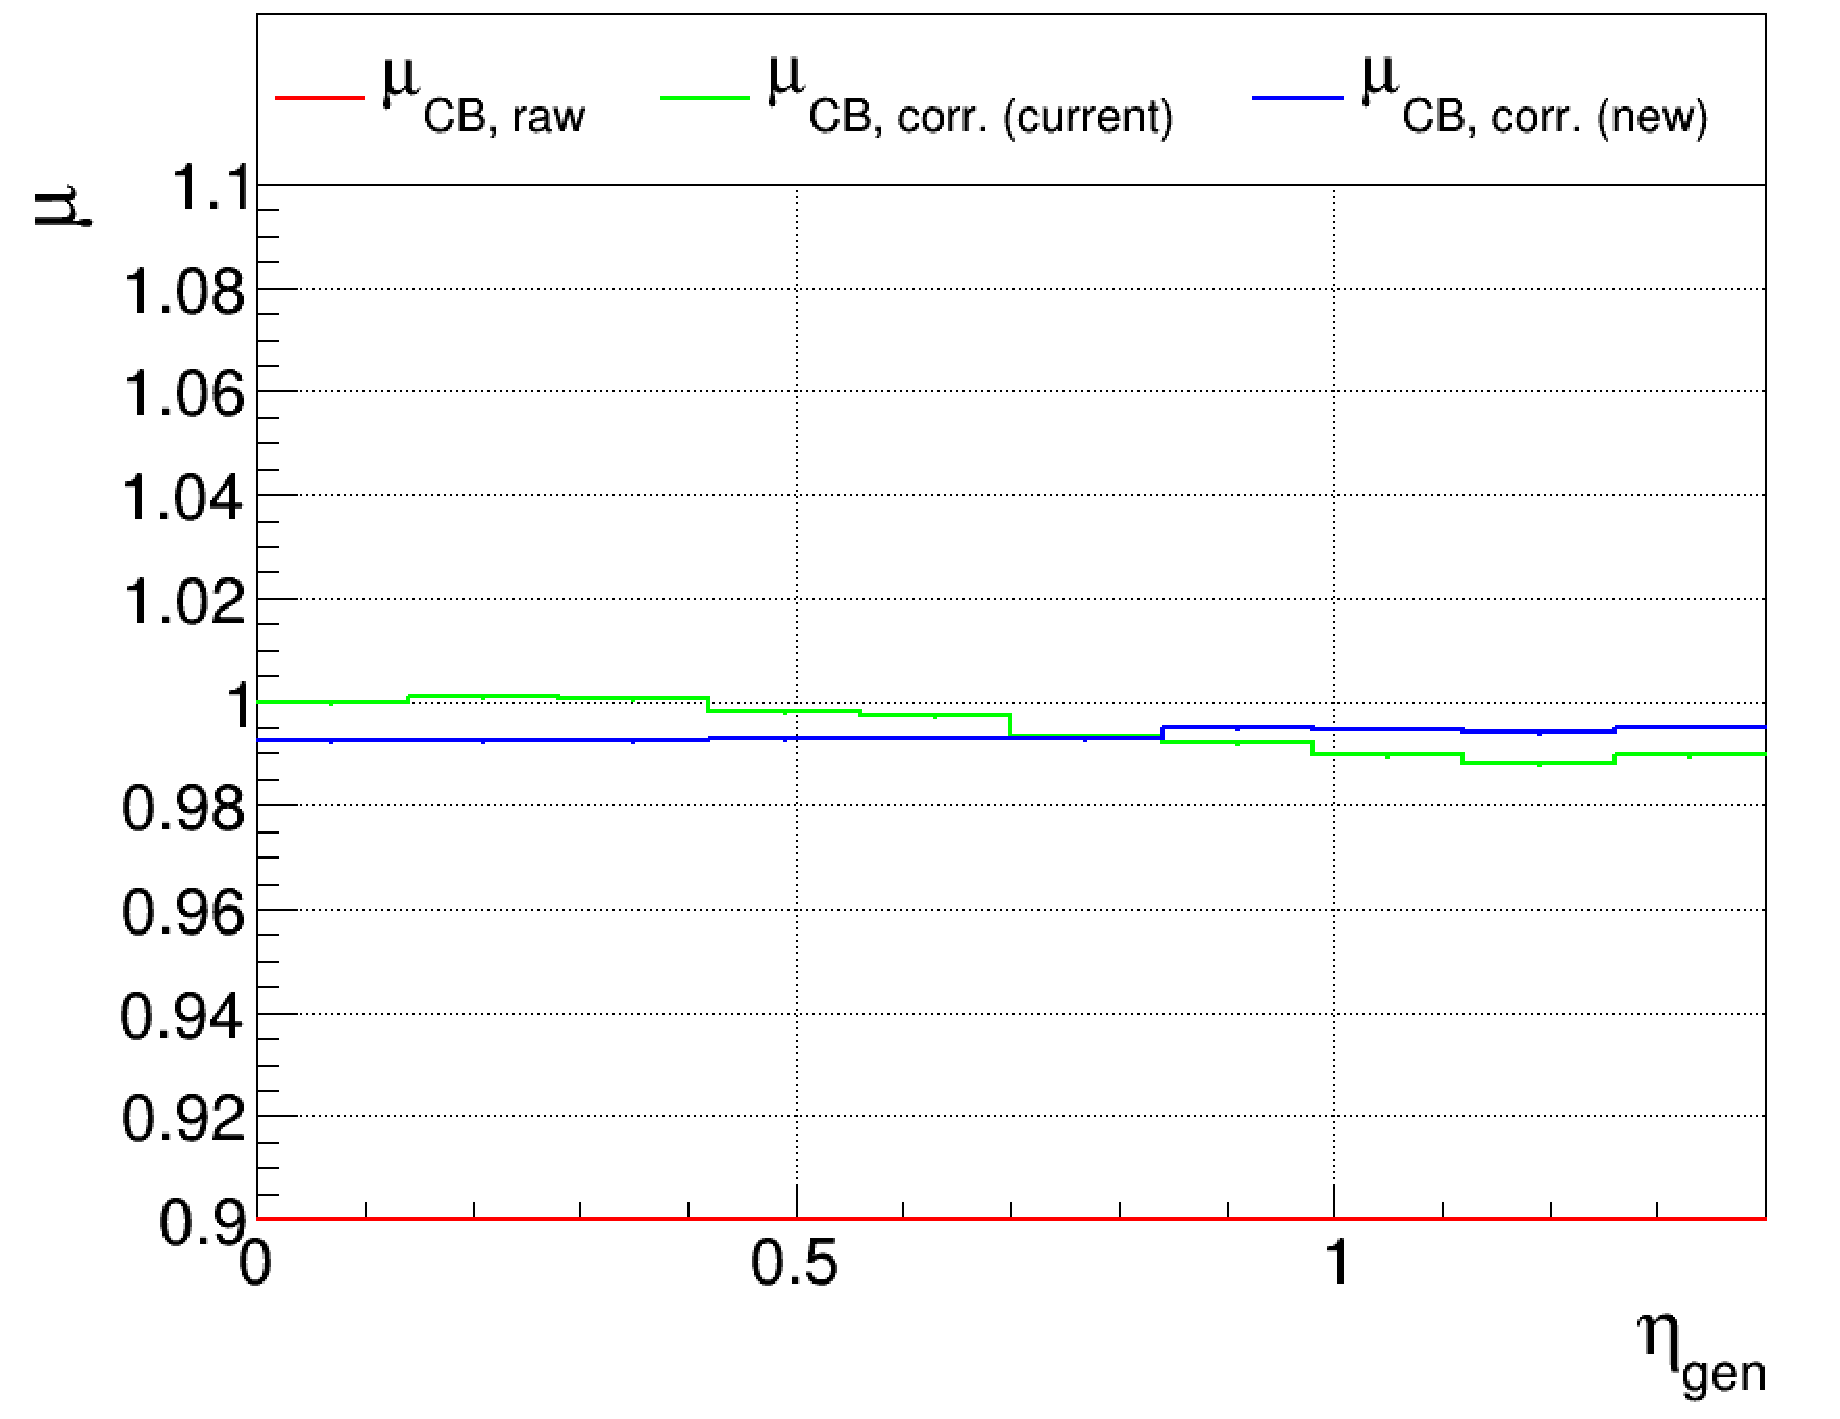
\includegraphics[width=0.495\textwidth]{./plots_pdf/ECAL_plots/plotsNOPU/EB/FULL/pdf/GENETA/EBFULL_GENETA_0005_0020_MuOverBins.pdf}
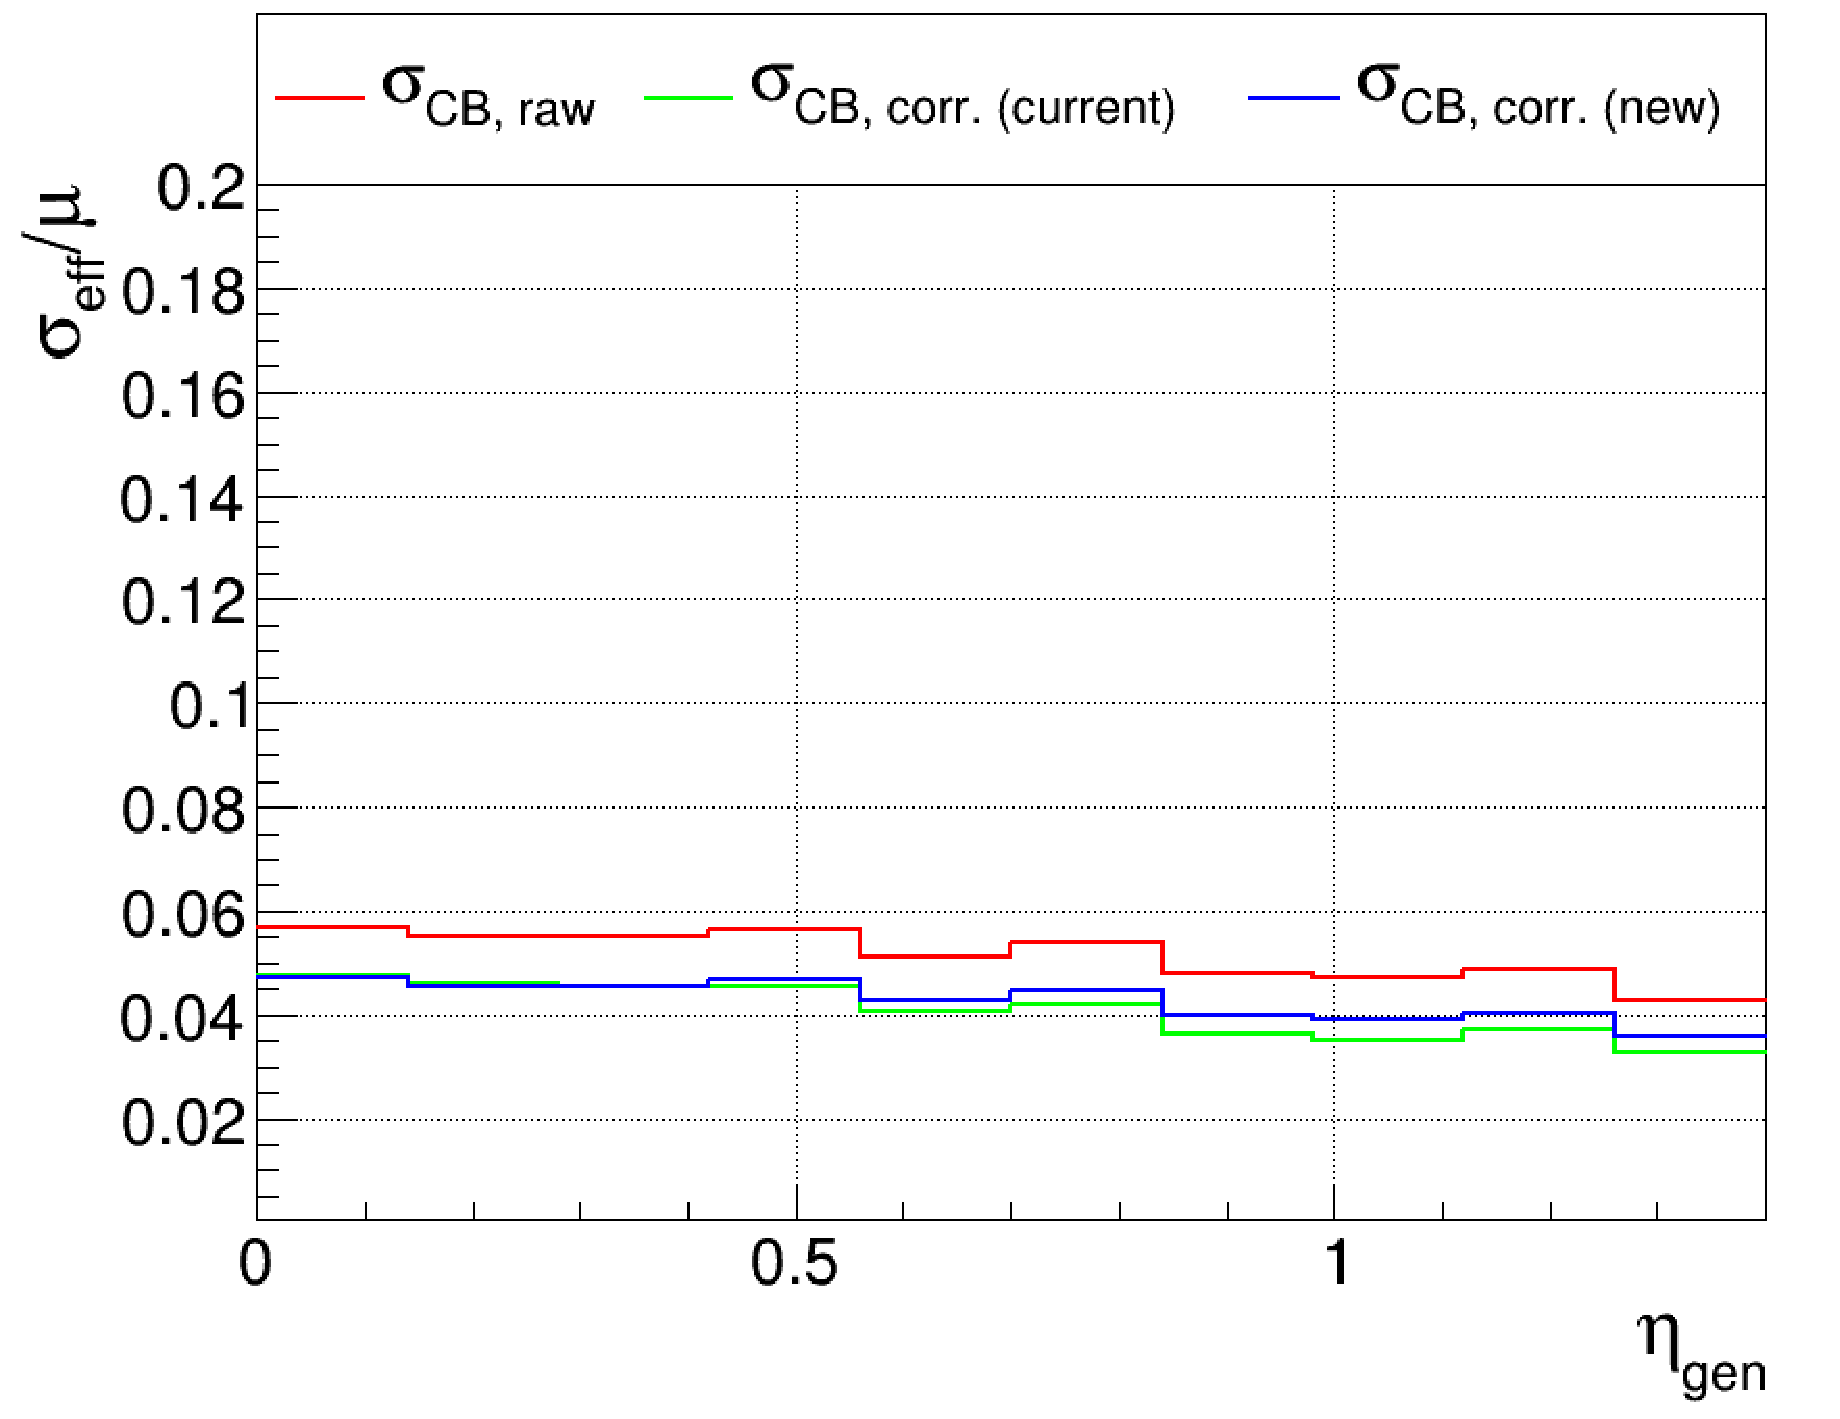
\includegraphics[width=0.495\textwidth]{./plots_pdf/ECAL_plots/plotsPU/EB/FULL/pdf/GENETA/EBFULL_GENETA_0005_0020_EffSigmaOverBins.pdf}
\caption{EB - Full Readout \pt 5-20}

%\begin{figure}
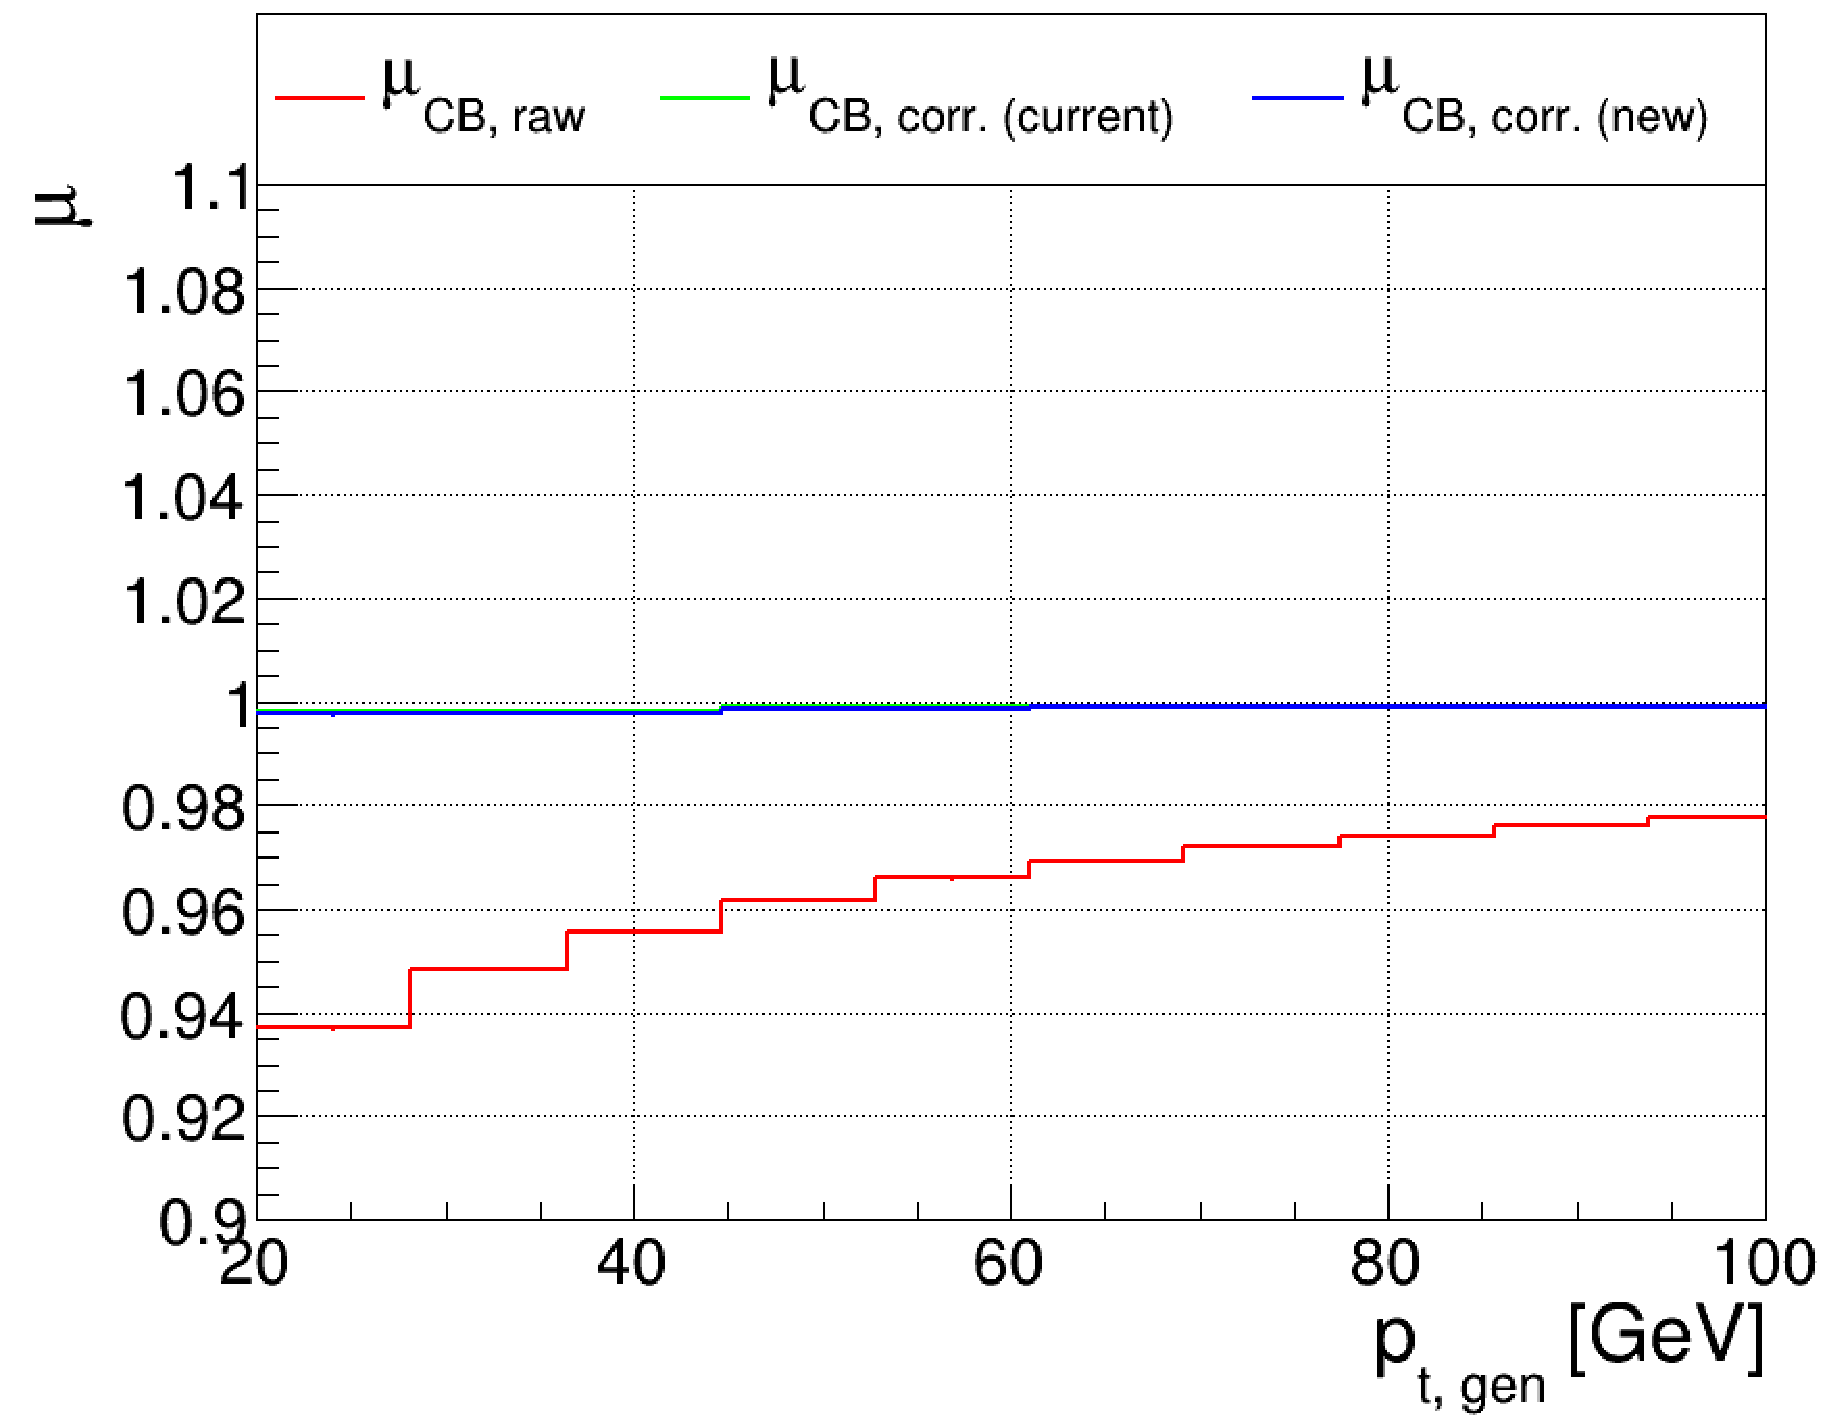
\includegraphics[width=0.495\textwidth]{./plots_pdf/ECAL_plots/plotsNOPU/EB/FULL/pdf/GENPT/EBFULL_GENPT_0020_0100_MuOverBins.pdf}
\includegraphics[width=0.495\textwidth]{./plots_pdf/ECAL_plots/plotsNOPU/EB/FULL/pdf/GENPT/EBFULL_GENPT_0020_0100_EffSigmaOverBins.pdf}

\includegraphics[width=0.495\textwidth]{./plots_pdf/ECAL_plots/plotsNOPU/EB/FULL/pdf/GENETA/EBFULL_GENETA_0020_0100_MuOverBins.pdf}
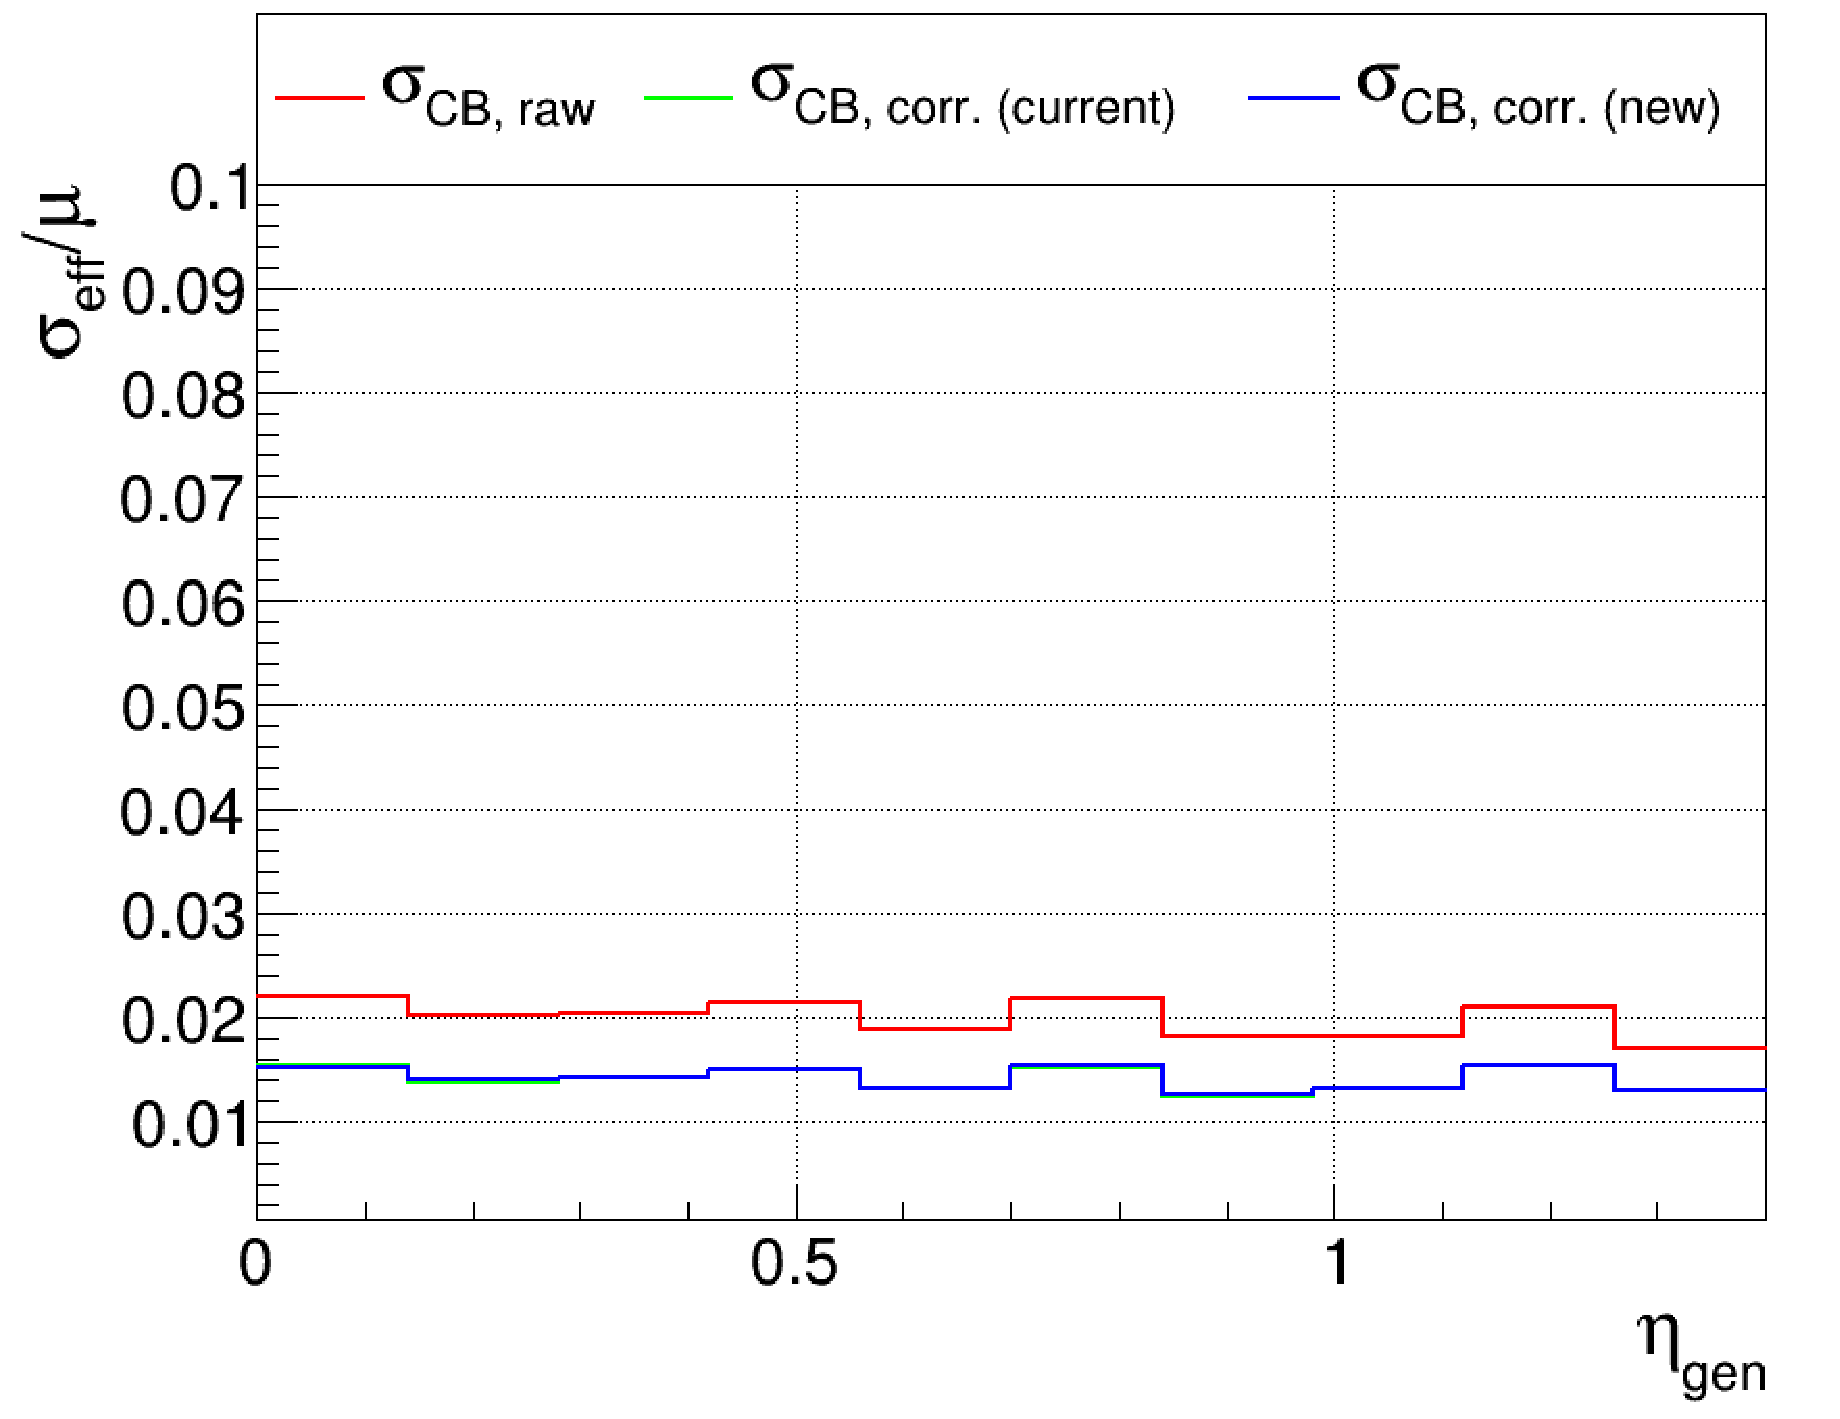
\includegraphics[width=0.495\textwidth]{./plots_pdf/ECAL_plots/plotsPU/EB/FULL/pdf/GENETA/EBFULL_GENETA_0020_0100_EffSigmaOverBins.pdf}
\caption{EB - Full Readout \pt 20-100}
\end{figure}


\begin{figure}
\includegraphics[width=0.495\textwidth]{./plots_pdf/ECAL_plots/plotsNOPU/EB/FULL/pdf/GENPT/EBFULL_GENPT_0100_0300_MuOverBins.pdf}
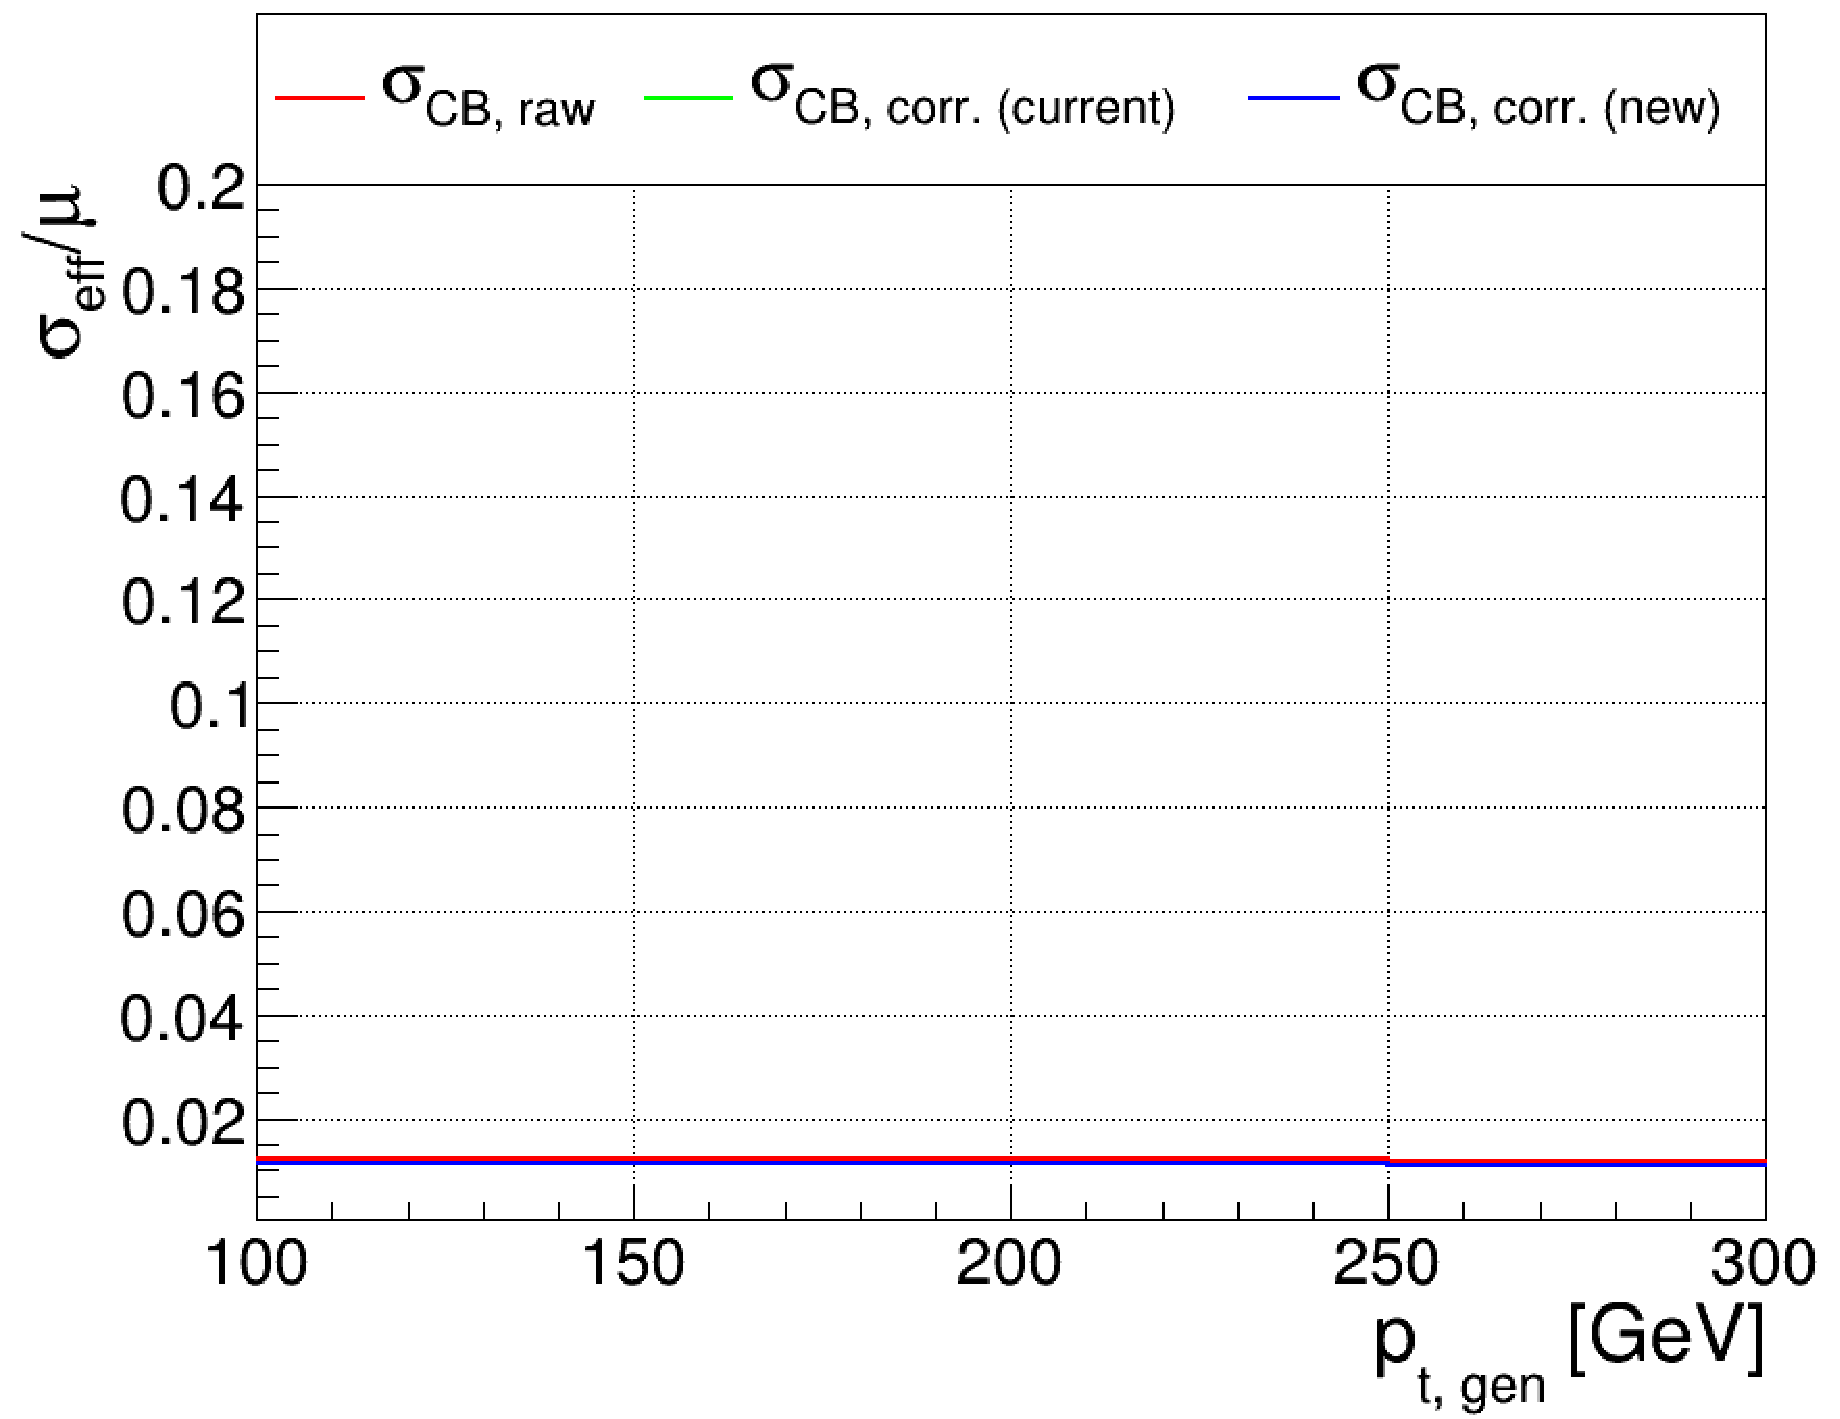
\includegraphics[width=0.495\textwidth]{./plots_pdf/ECAL_plots/plotsPU/EB/FULL/pdf/GENPT/EBFULL_GENPT_0100_0300_EffSigmaOverBins.pdf}


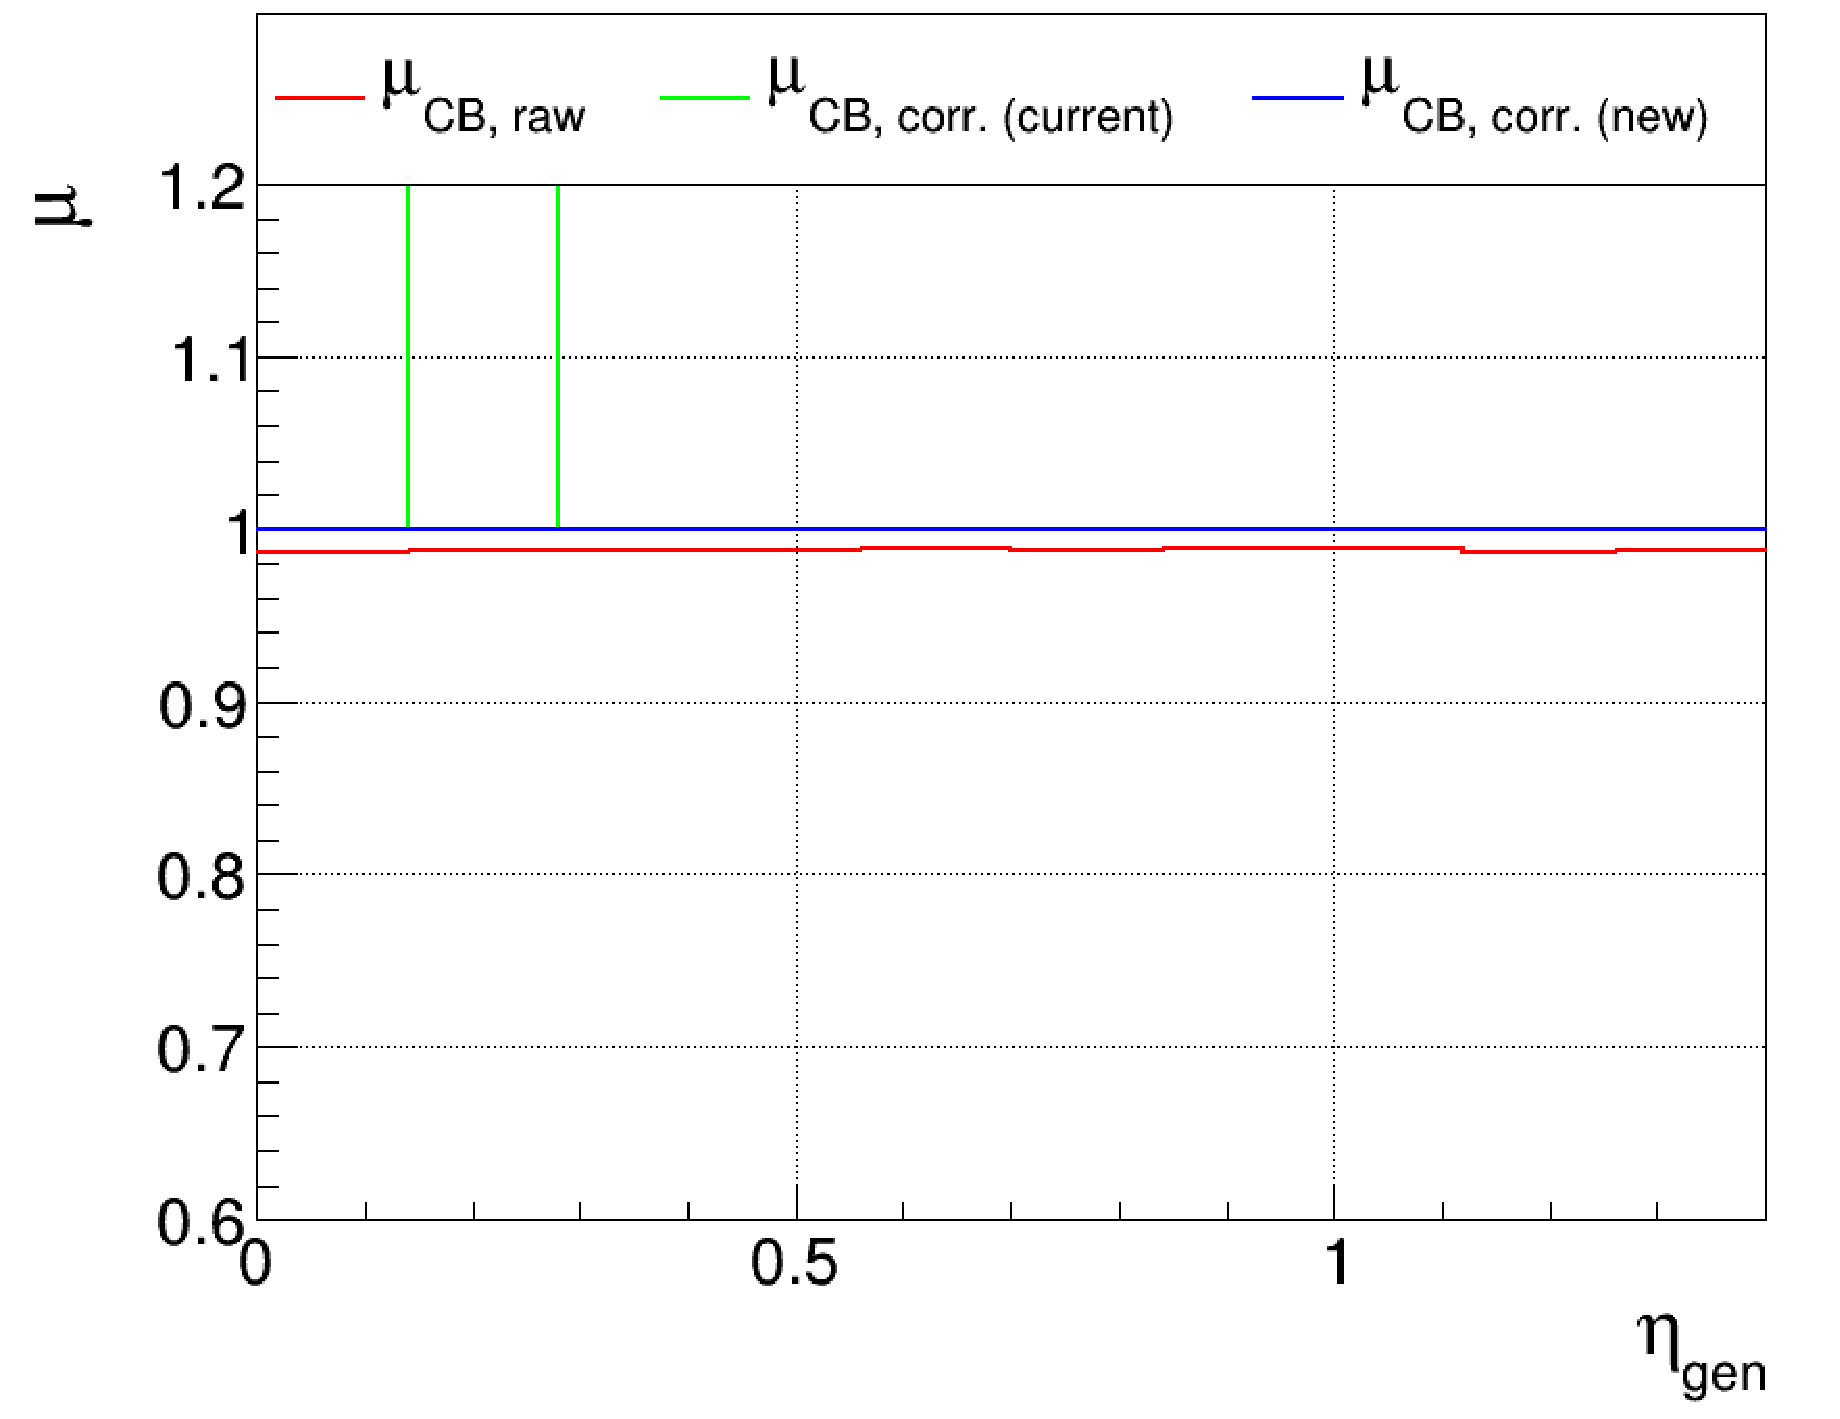
\includegraphics[width=0.495\textwidth]{./plots_pdf/ECAL_plots/plotsNOPU/EB/FULL/pdf/GENETA/EBFULL_GENETA_0100_0300_MuOverBins.pdf}
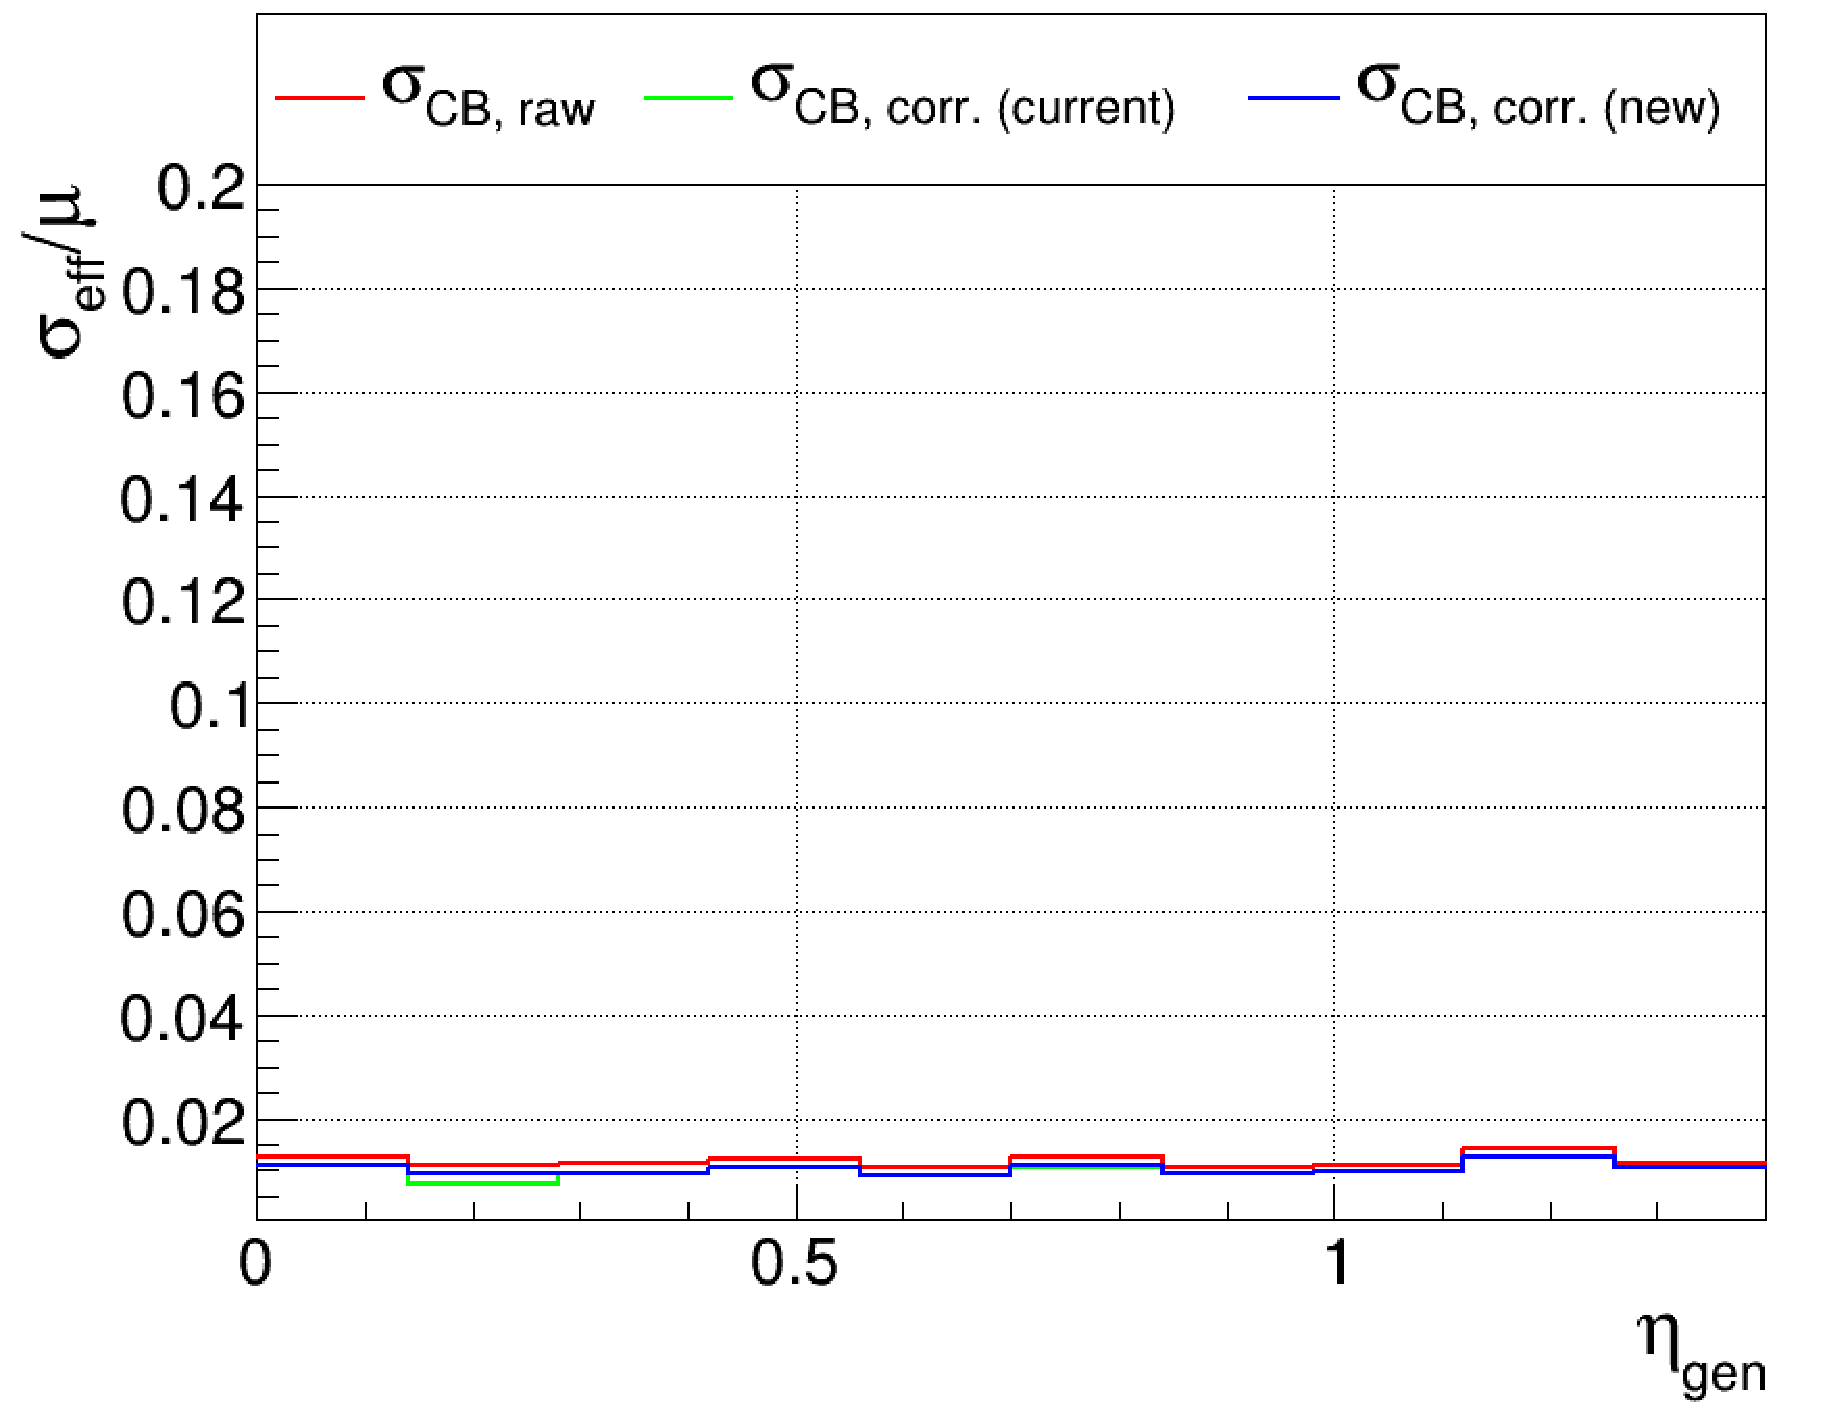
\includegraphics[width=0.495\textwidth]{./plots_pdf/ECAL_plots/plotsNOPU/EB/FULL/pdf/GENETA/EBFULL_GENETA_0100_0300_EffSigmaOverBins.pdf}
\caption{EB - Full Readout \pt 100-300}
\end{figure}




\begin{figure}
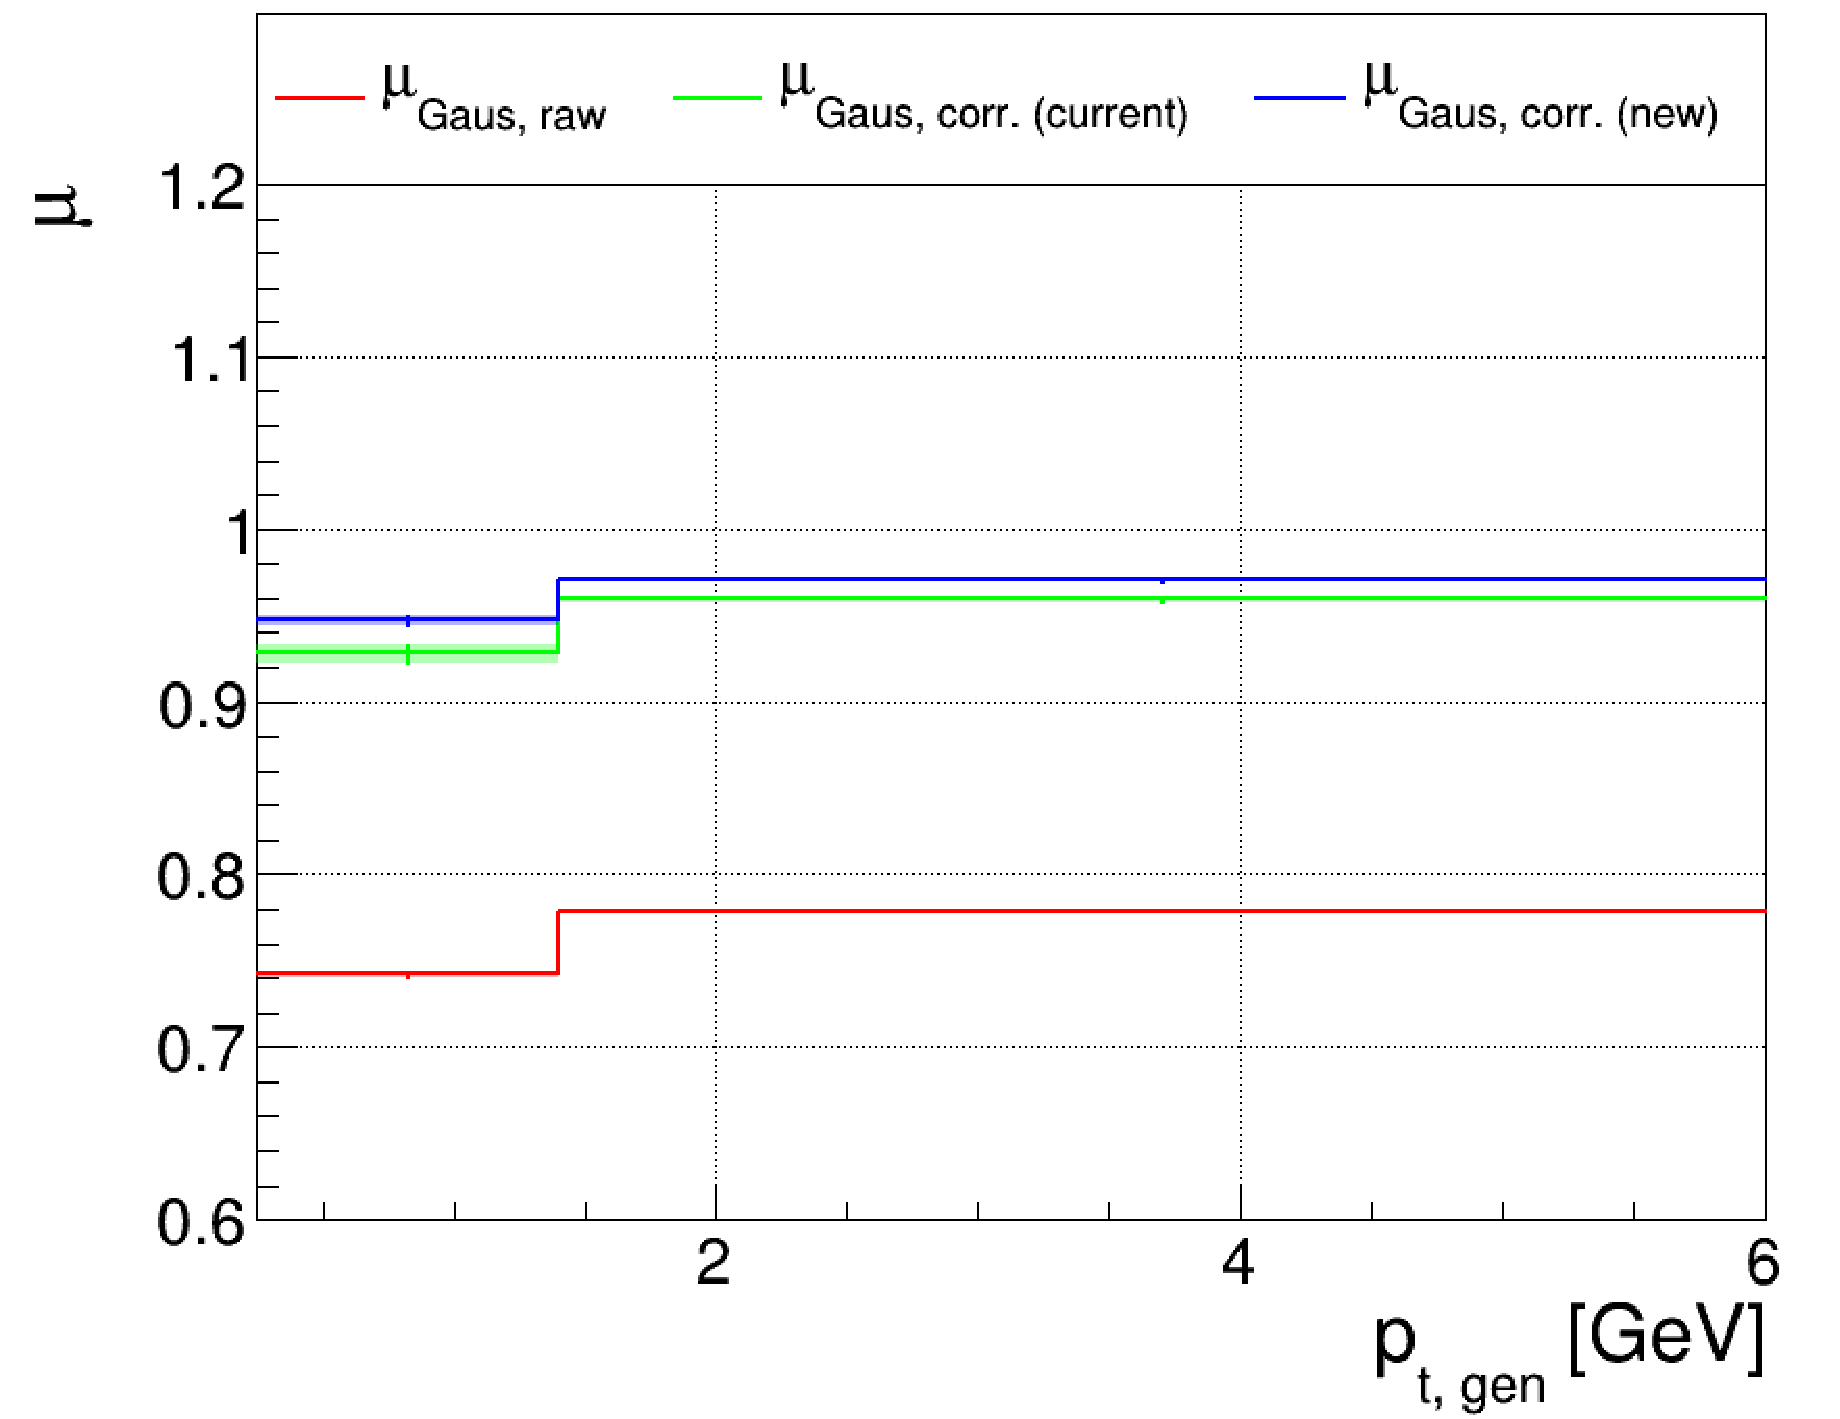
\includegraphics[width=0.495\textwidth]{./plots_pdf/ECAL_plots/plotsNOPU/EB/ZS/pdf/GENPT/EBZS_GENPT_0000_0006_MuOverBins.pdf}
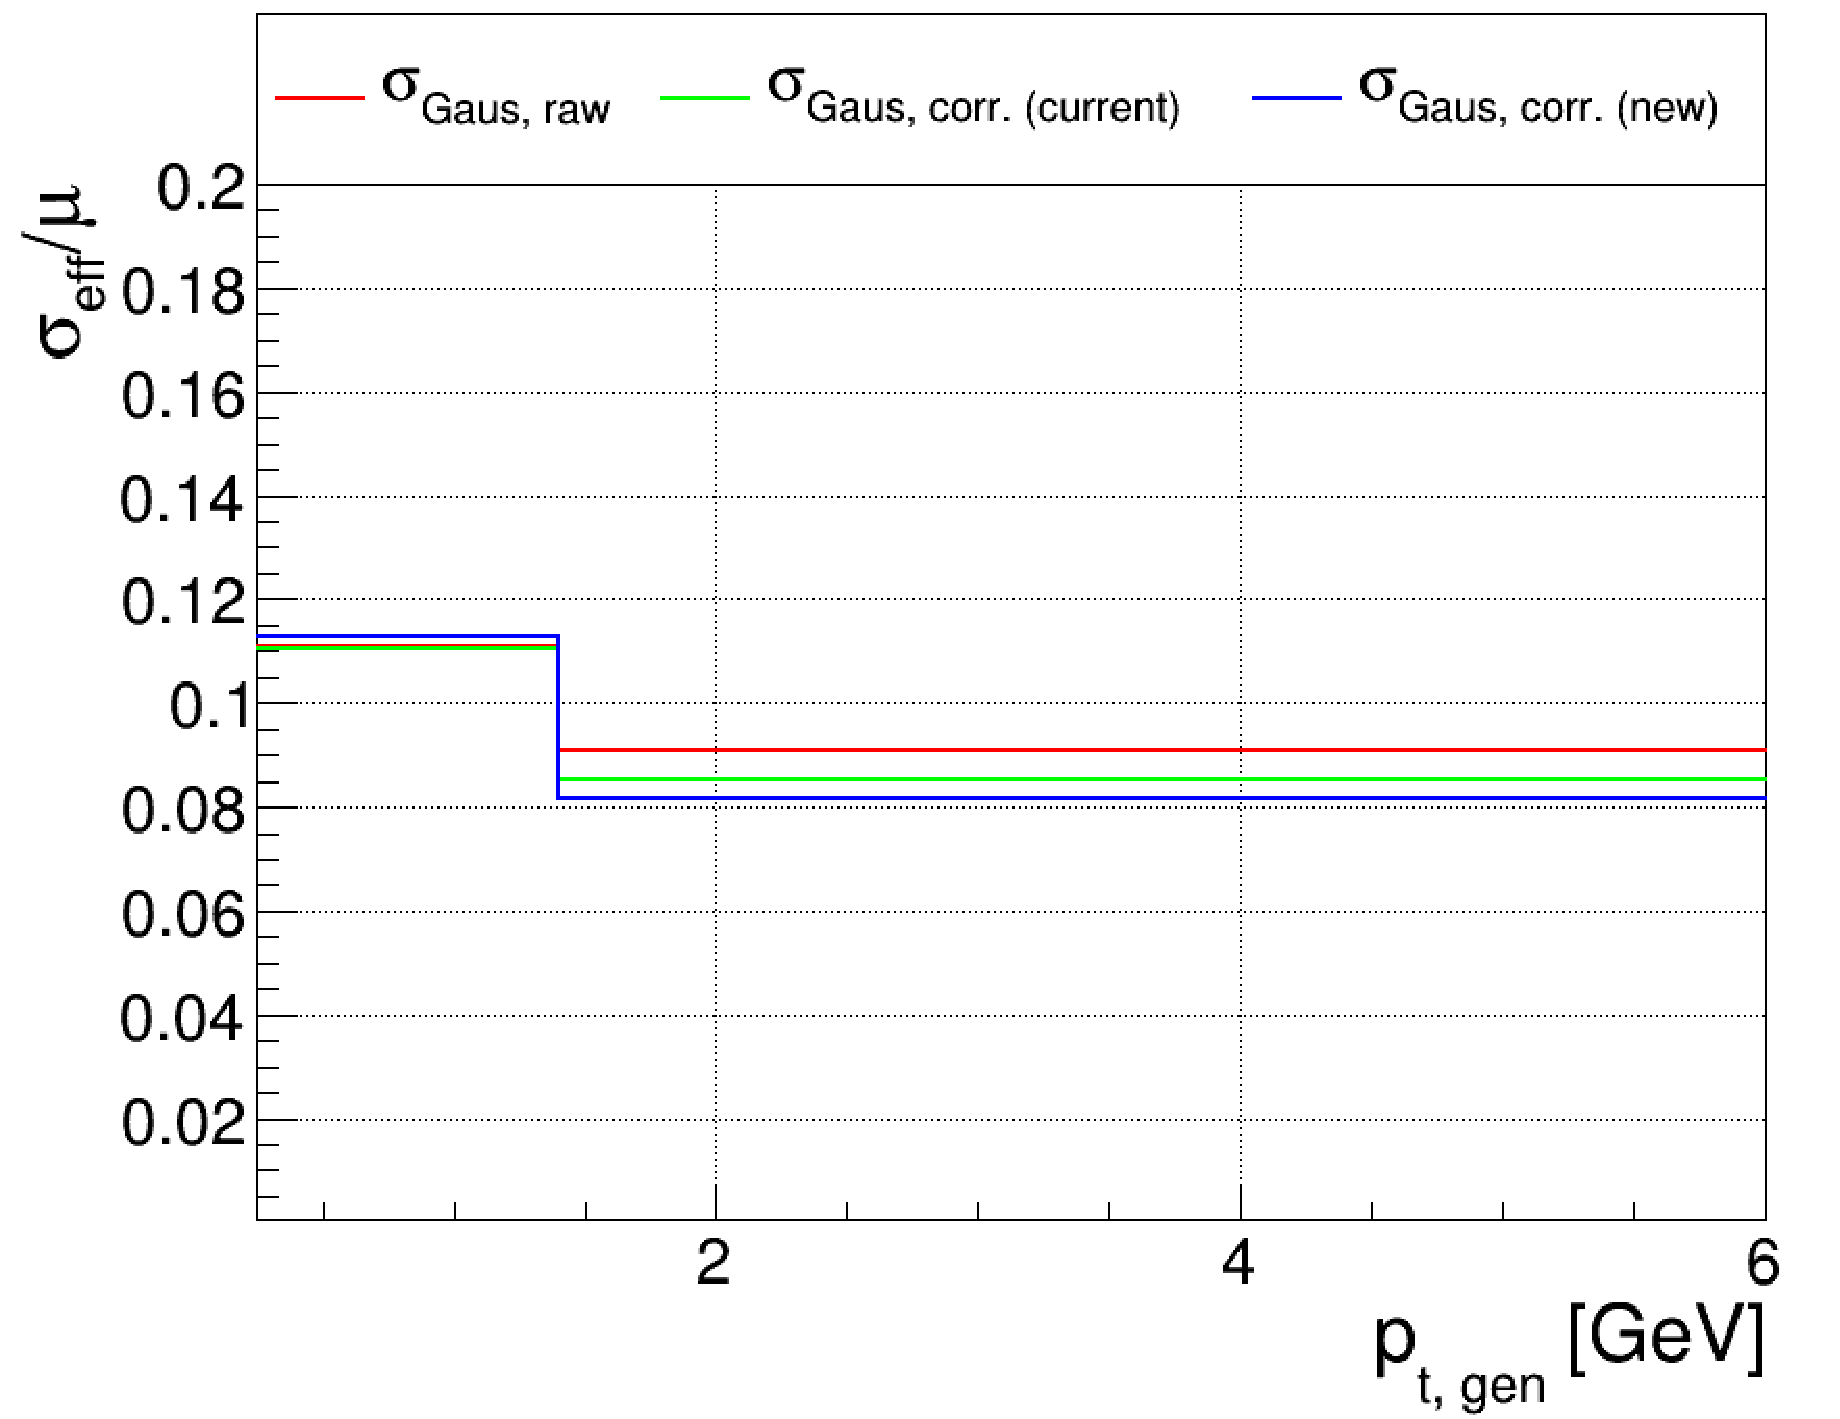
\includegraphics[width=0.495\textwidth]{./plots_pdf/ECAL_plots/plotsNOPU/EB/ZS/pdf/GENPT/EBZS_GENPT_0000_0006_EffSigmaOverBins.pdf}

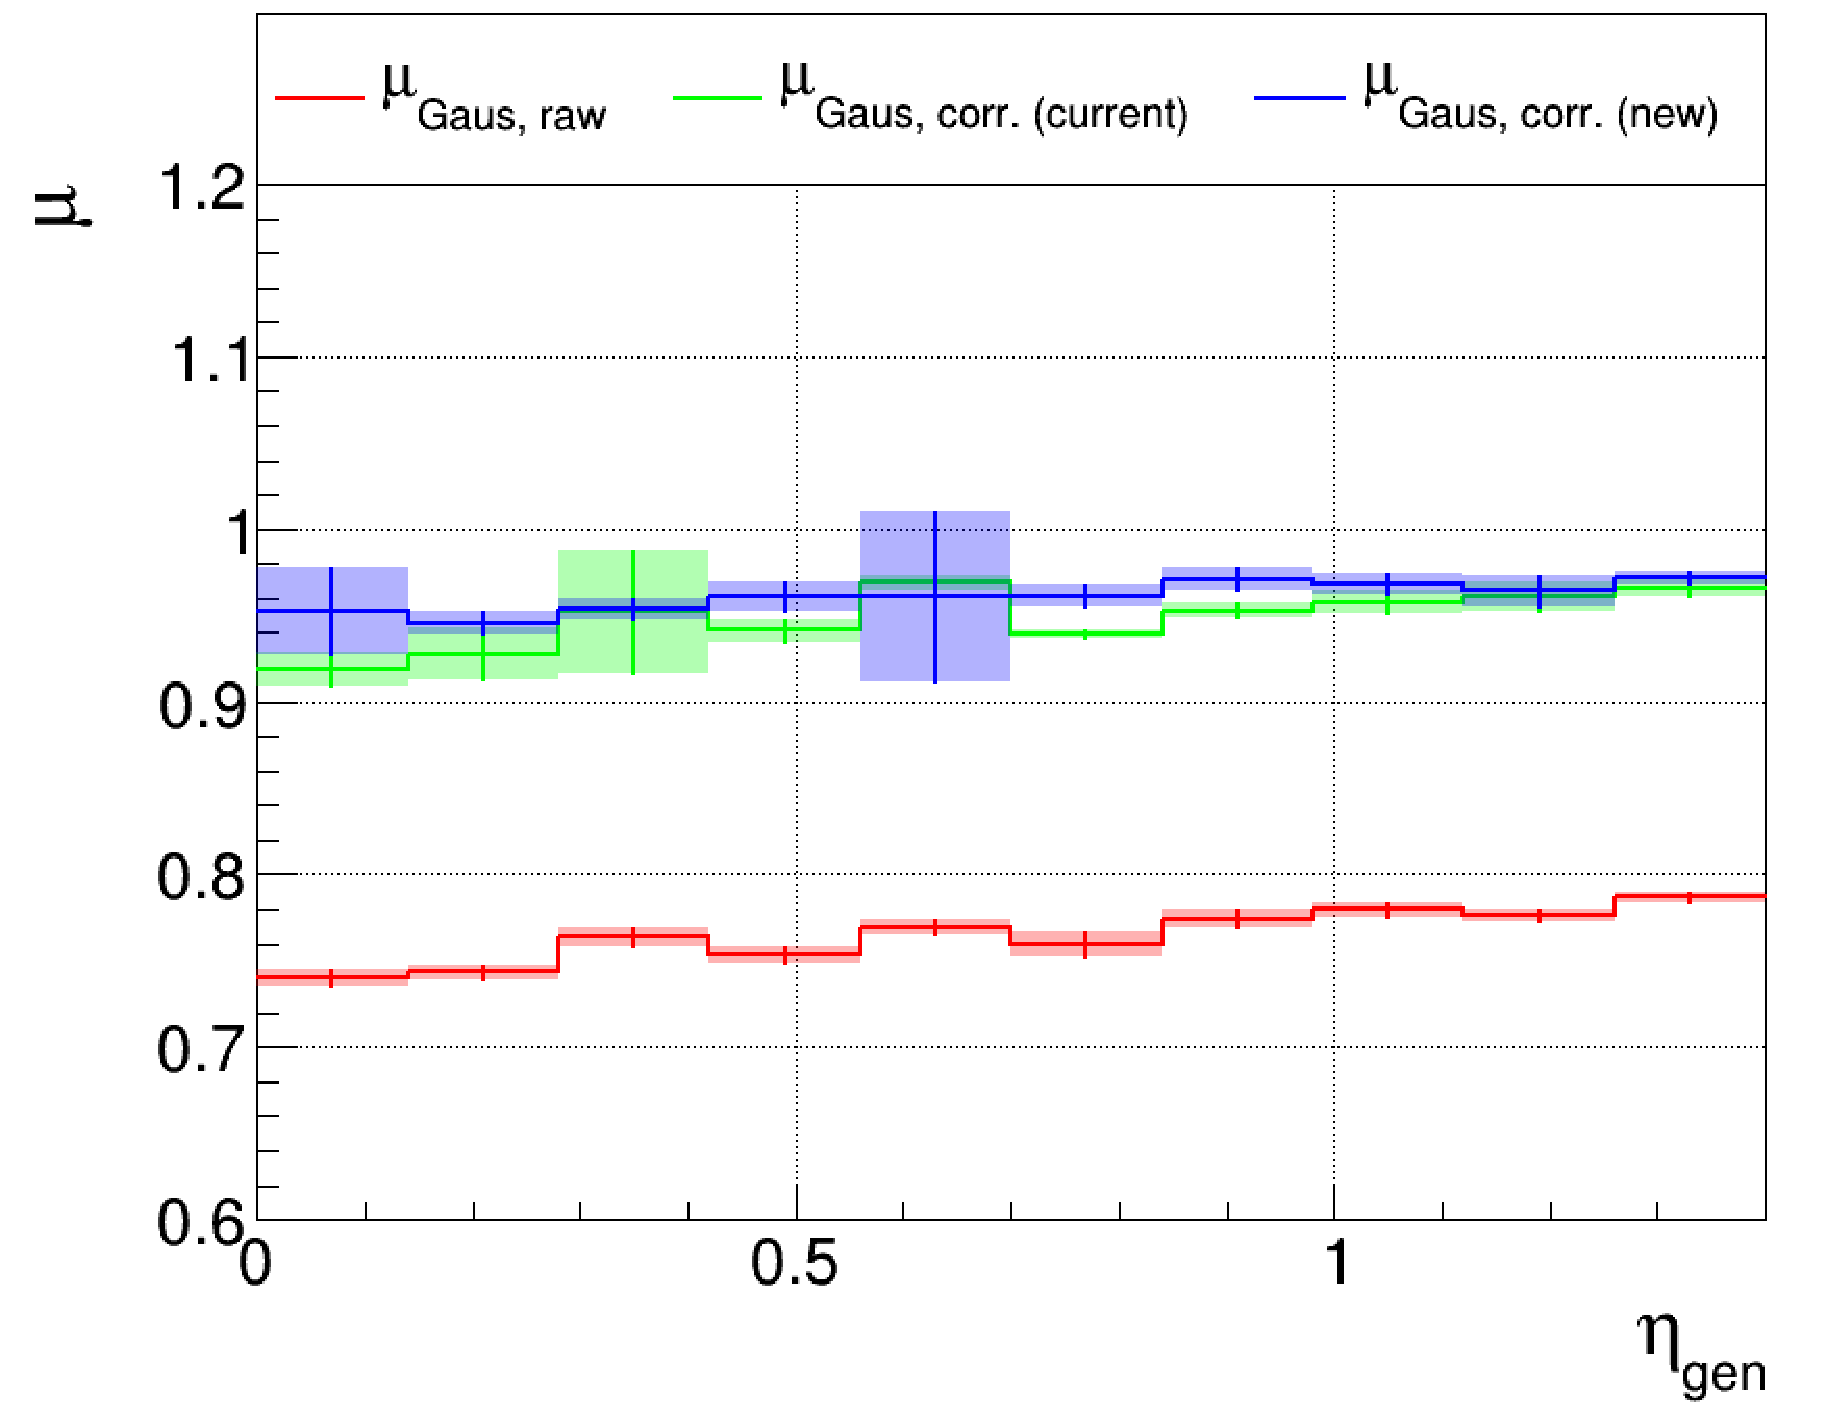
\includegraphics[width=0.495\textwidth]{./plots_pdf/ECAL_plots/plotsNOPU/EB/ZS/pdf/GENETA/EBZS_GENETA_0000_0006_MuOverBins.pdf}
\includegraphics[width=0.495\textwidth]{./plots_pdf/ECAL_plots/plotsNOPU/EB/ZS/pdf/GENETA/EBZS_GENETA_0000_0006_EffSigmaOverBins.pdf}
\caption[]{EB - ZS Readout \pt 0--6\GeV.}
\end{figure}

%% \begin{figure}
%% \includegraphics[width=0.495\textwidth]{./plots_pdf/ECAL_plots/plotsNOPU/EB/ZS/pdf/GENPT/EBZS_GENPT_0006_0025_MuOverBins.pdf}
%% 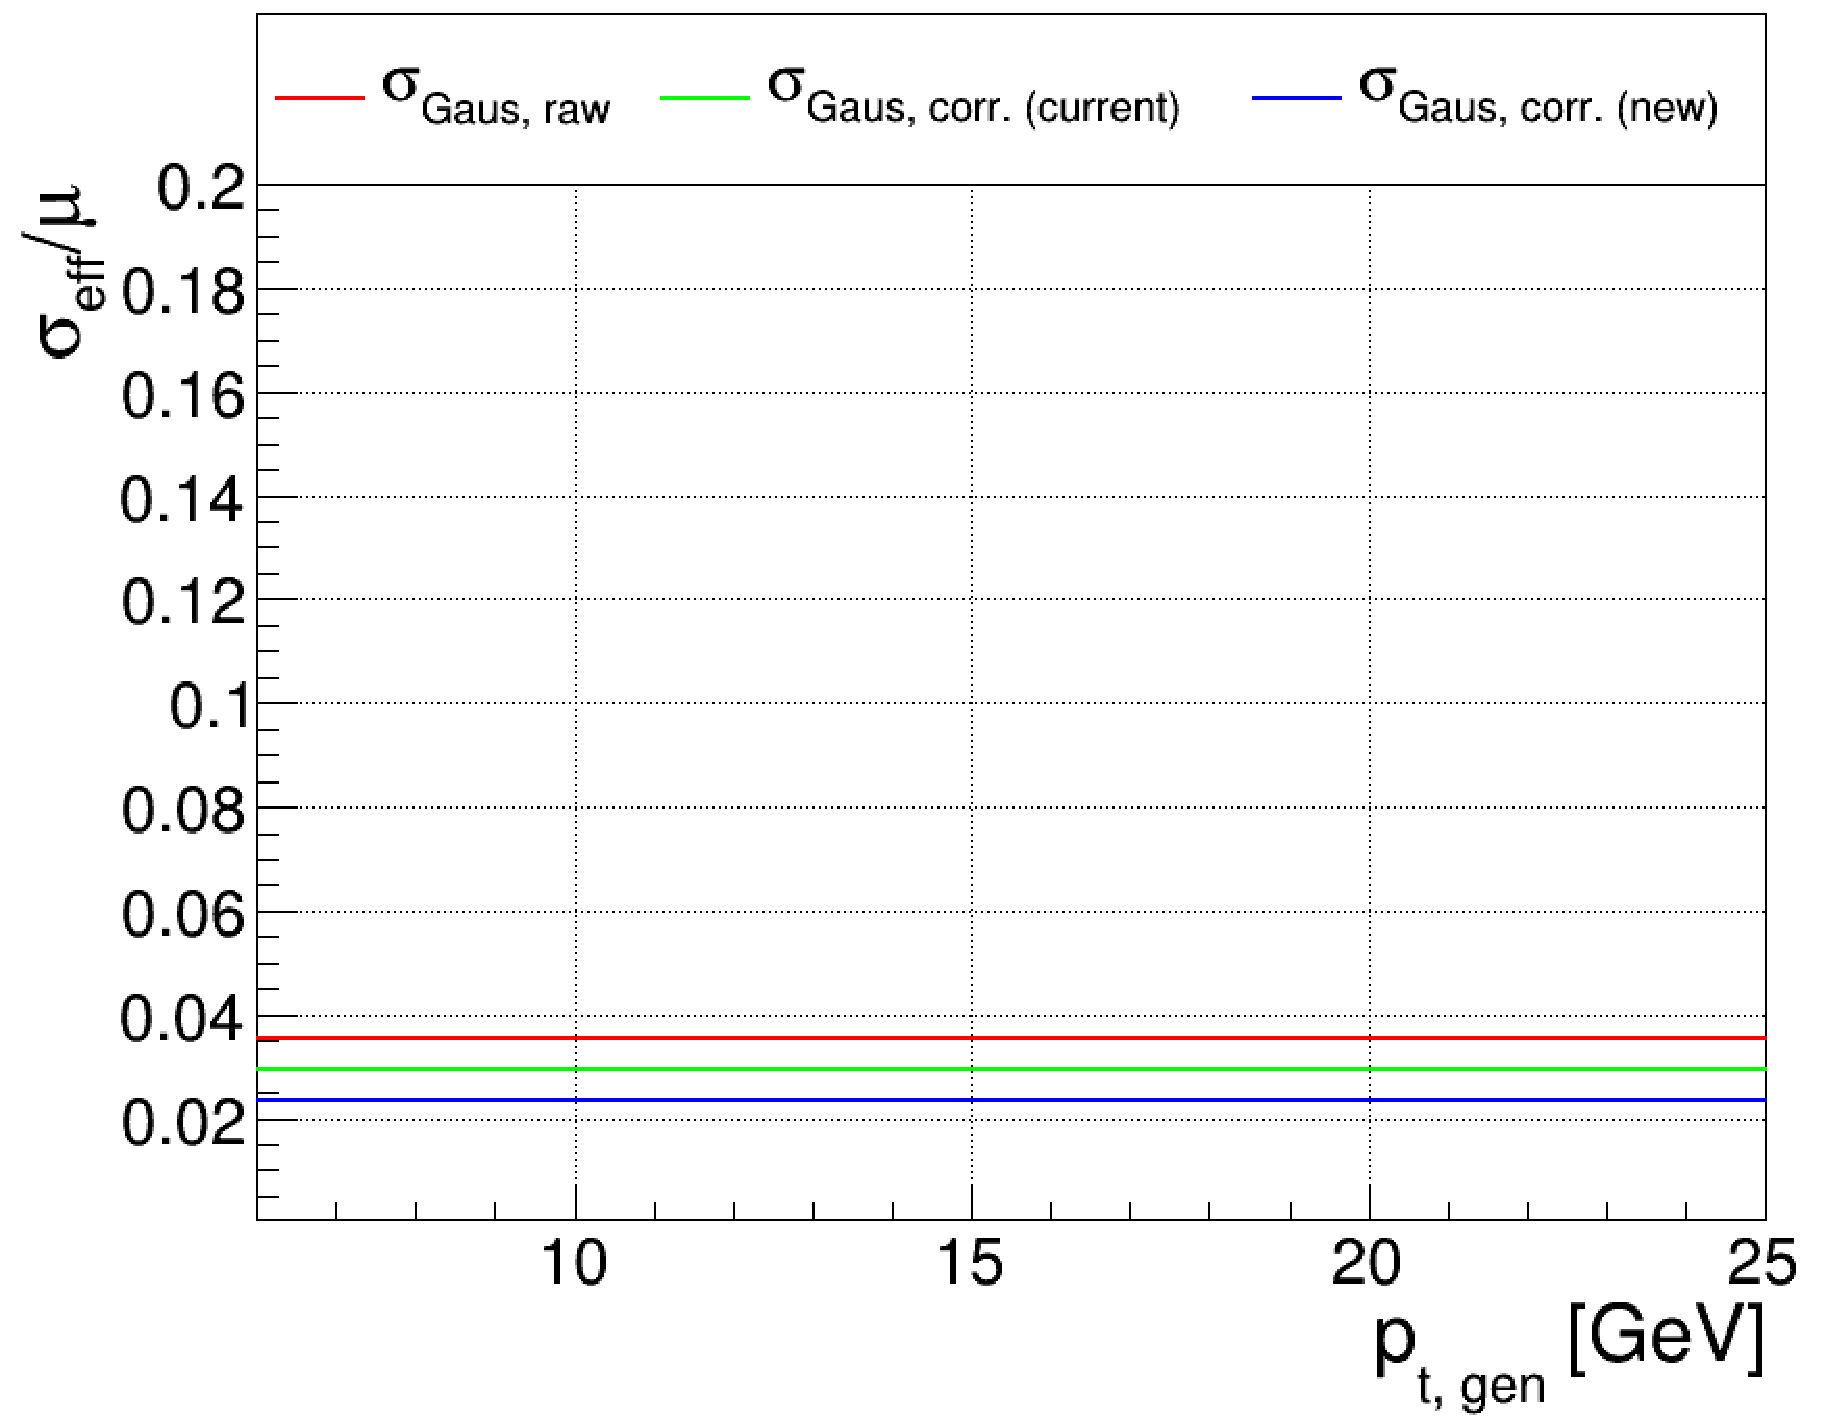
\includegraphics[width=0.495\textwidth]{./plots_pdf/ECAL_plots/plotsNOPU/EB/ZS/pdf/GENPT/EBZS_GENPT_0006_0025_EffSigmaOverBins.pdf}

%% 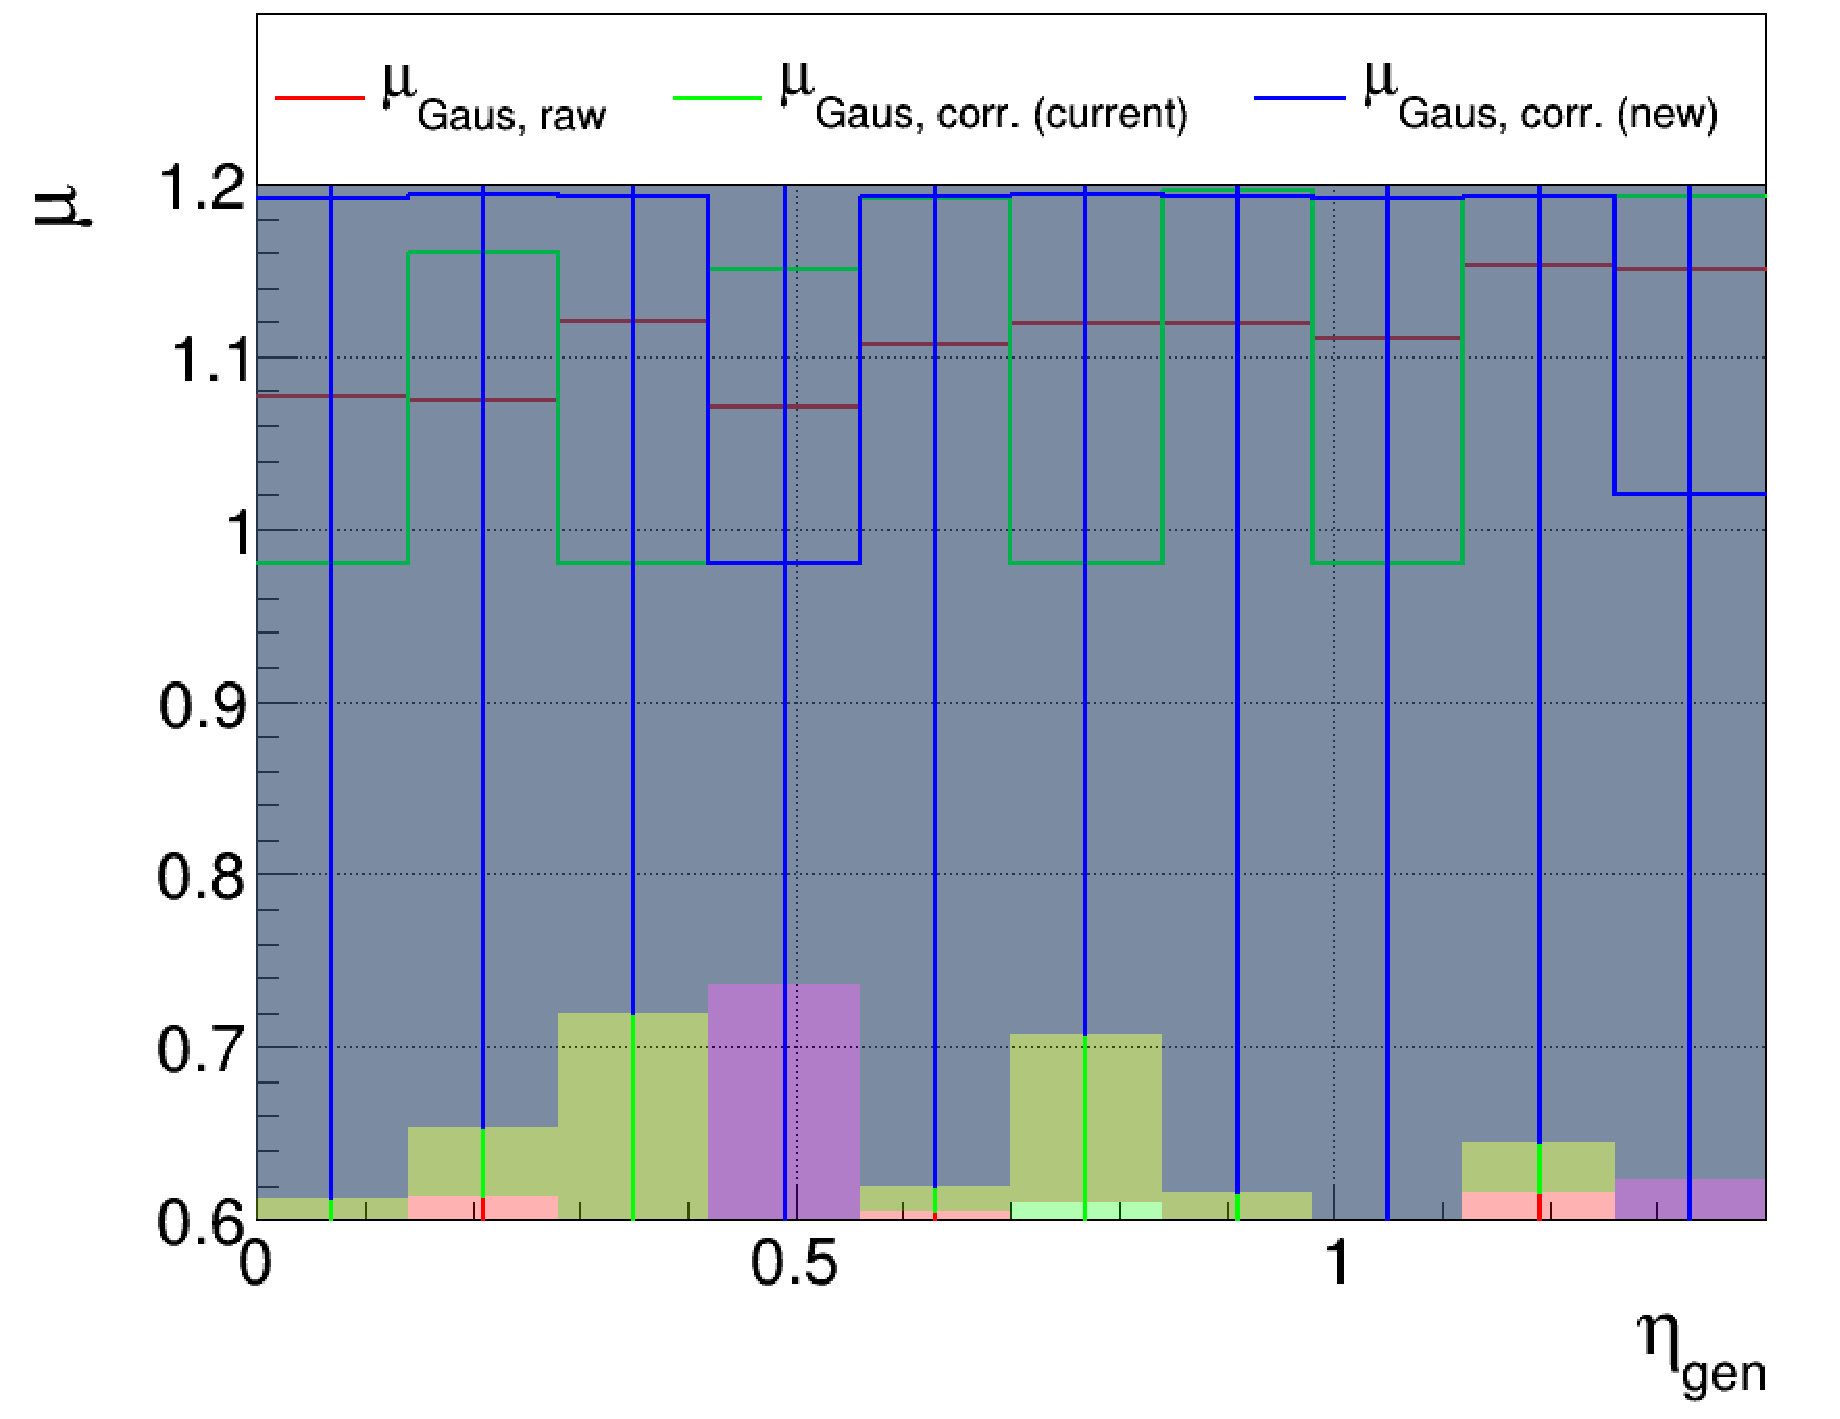
\includegraphics[width=0.495\textwidth]{./plots_pdf/ECAL_plots/plotsNOPU/EB/ZS/pdf/GENETA/EBZS_GENETA_0006_0025_MuOverBins.pdf}
%% 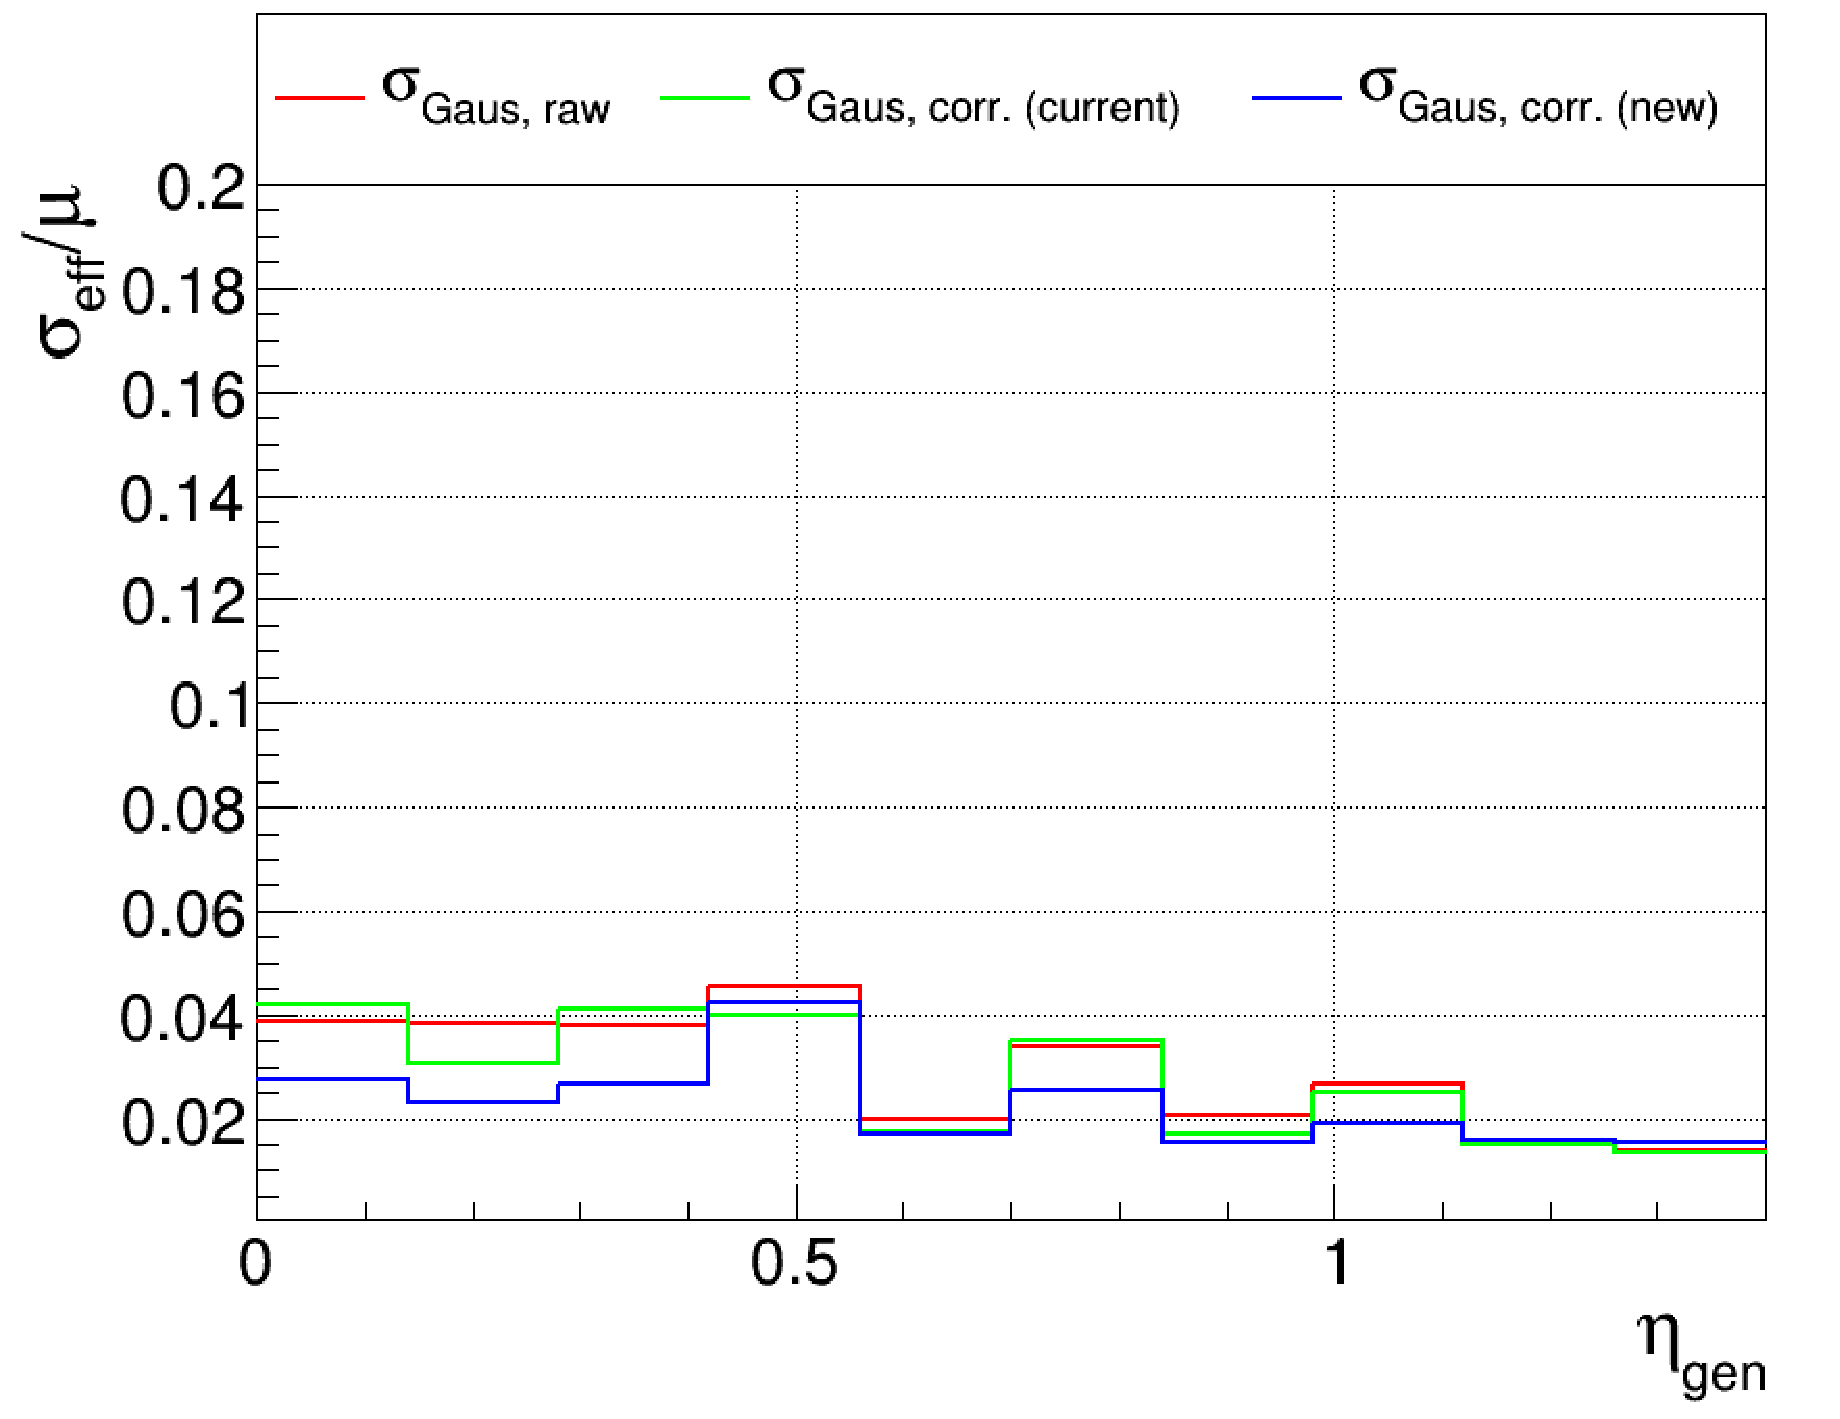
\includegraphics[width=0.495\textwidth]{./plots_pdf/ECAL_plots/plotsNOPU/EB/ZS/pdf/GENETA/EBZS_GENETA_0006_0025_EffSigmaOverBins.pdf}
%% \caption[]{EB - ZS Readout \pt 6-25\GeV}
%% \end{figure}





\begin{figure}
\includegraphics[width=0.495\textwidth]{./plots_pdf/ECAL_plots/plotsPU/EB/FULL/pdf/GENPT/EBFULL_GENPT_0005_0020_MuOverBins.pdf}
\includegraphics[width=0.495\textwidth]{./plots_pdf/ECAL_plots/plotsPU/EB/FULL/pdf/GENPT/EBFULL_GENPT_0005_0020_EffSigmaOverBins.pdf}
%\caption{EB - Full Readout pt 5-20}
%\end{figure}
%\begin{figure}
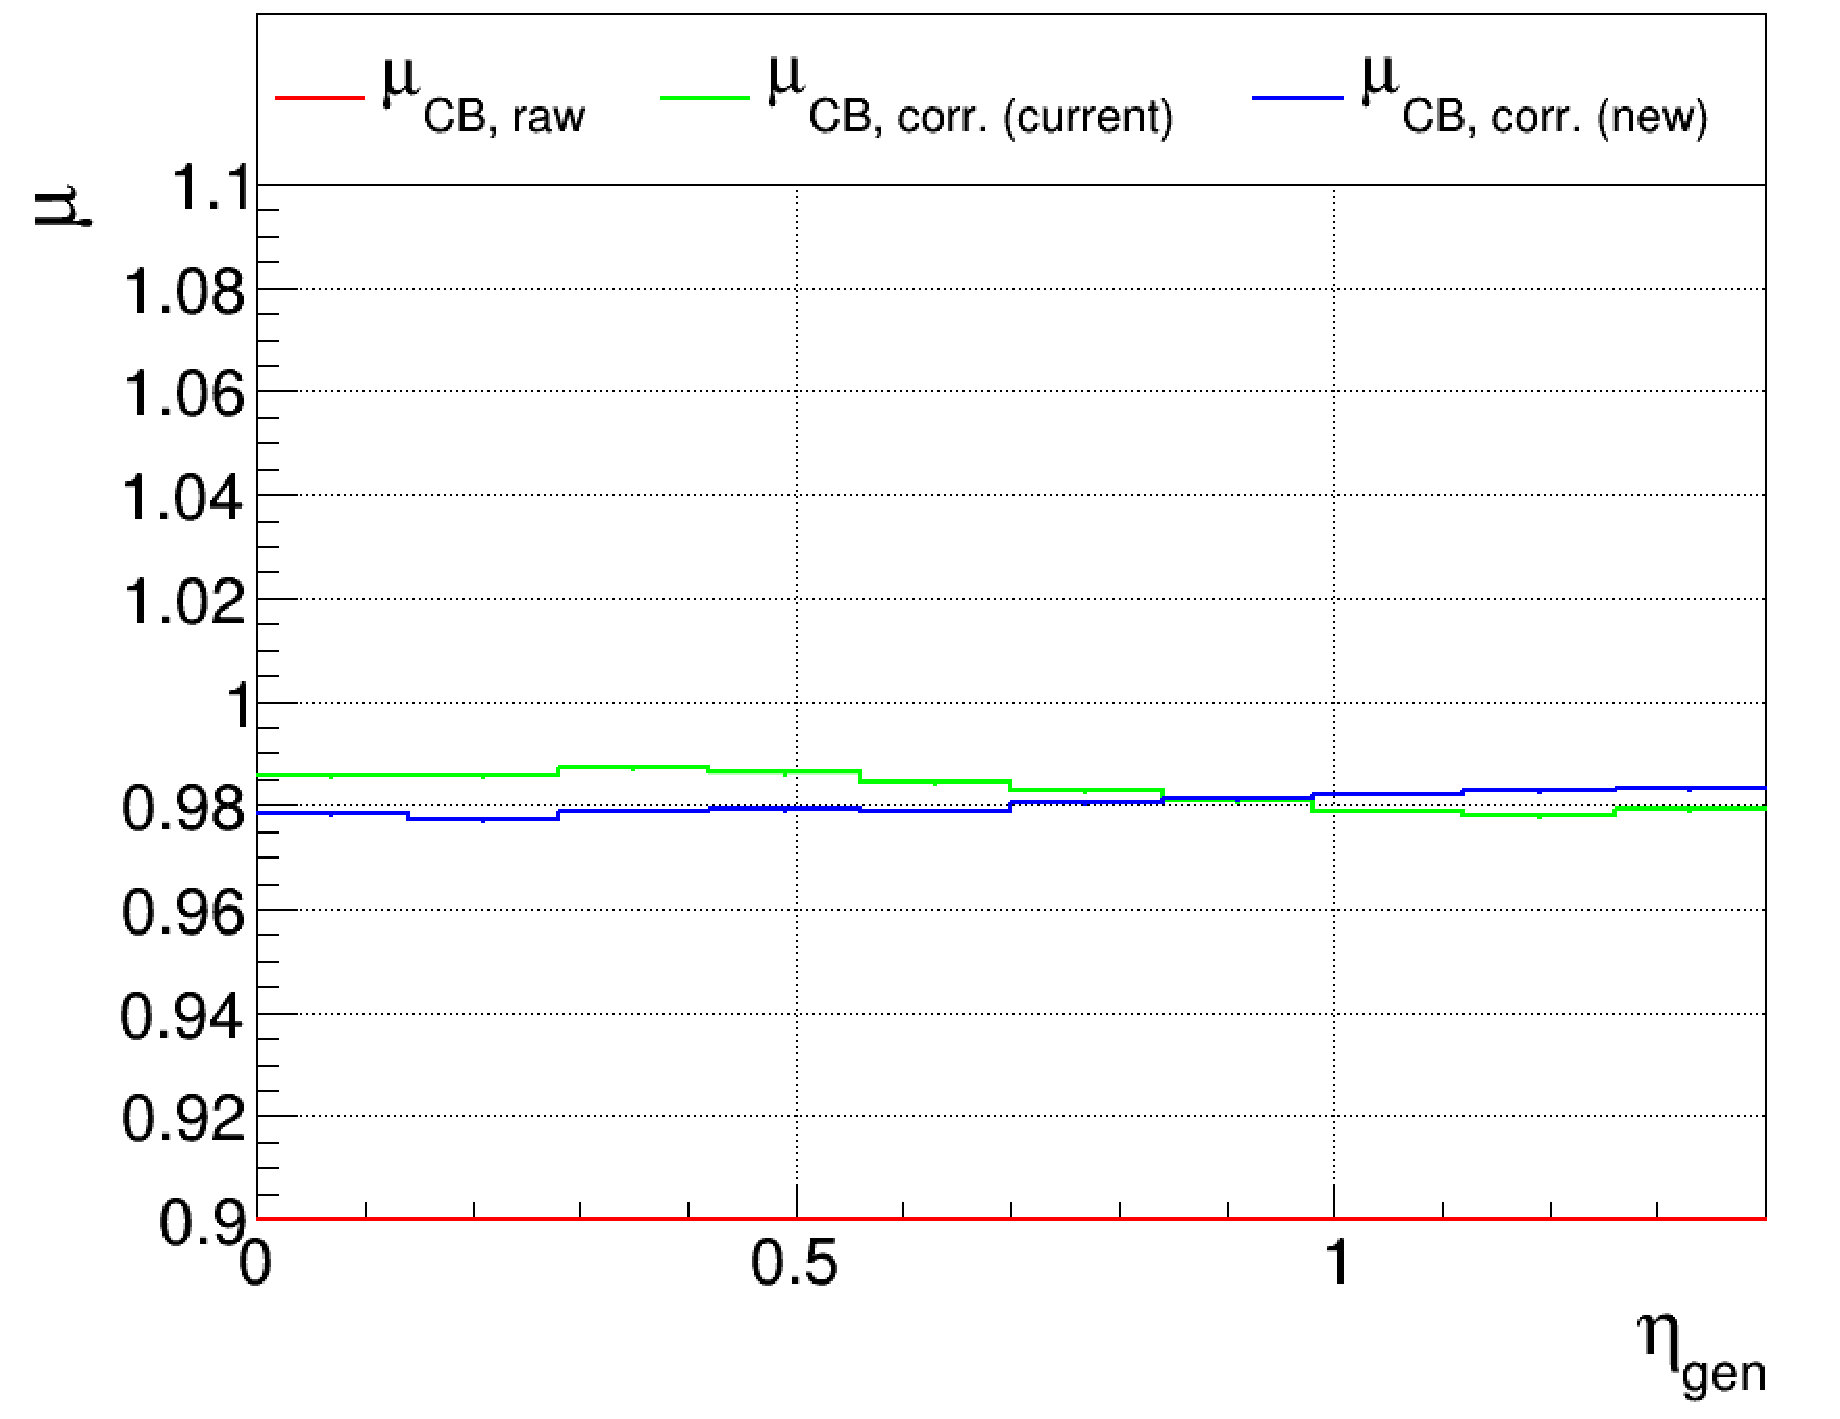
\includegraphics[width=0.495\textwidth]{./plots_pdf/ECAL_plots/plotsPU/EB/FULL/pdf/GENETA/EBFULL_GENETA_0005_0020_MuOverBins.pdf}
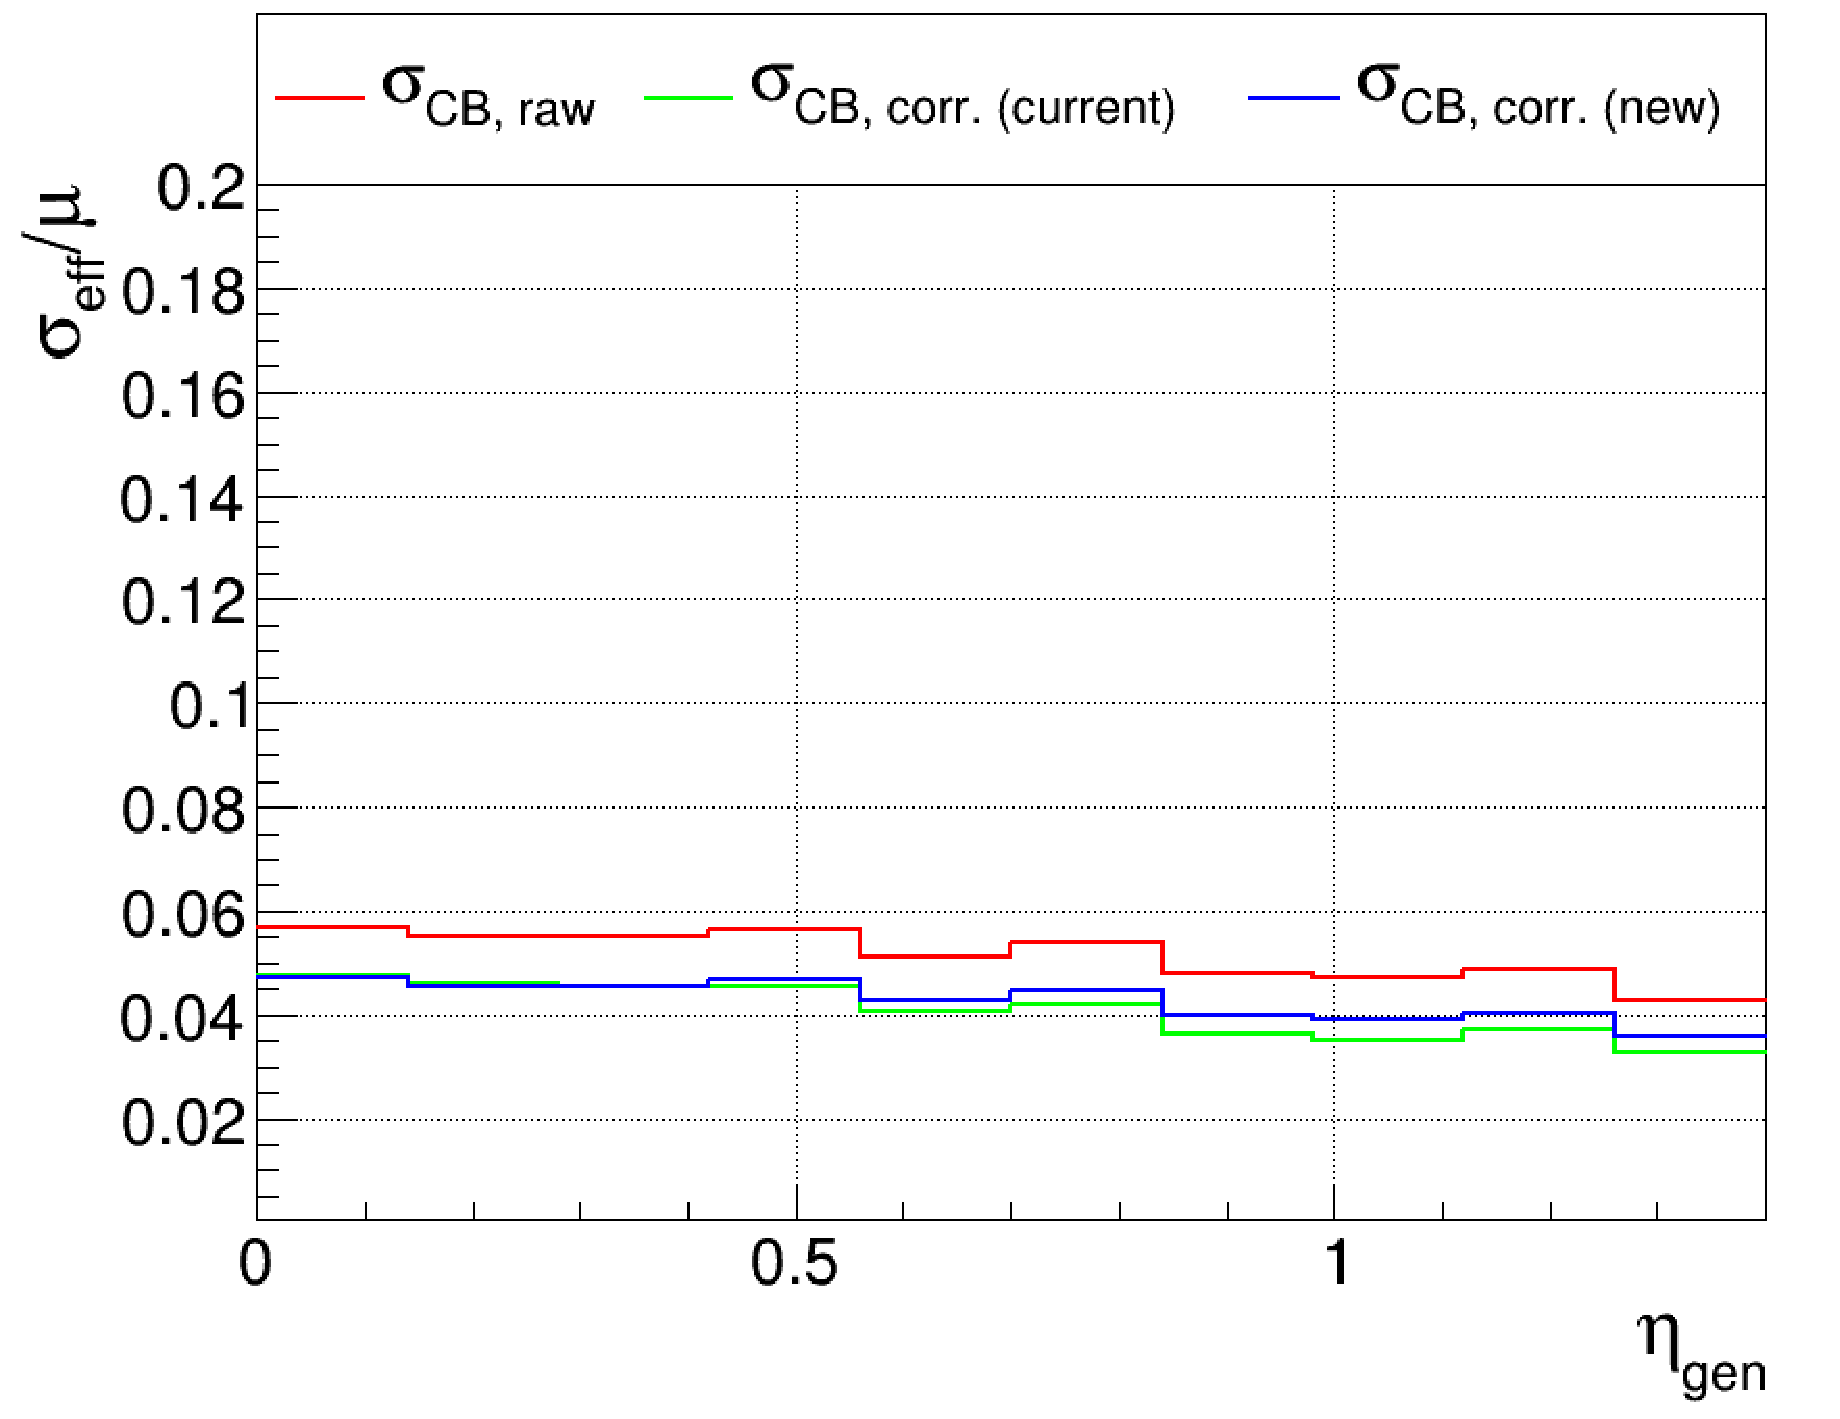
\includegraphics[width=0.495\textwidth]{./plots_pdf/ECAL_plots/plotsPU/EB/FULL/pdf/GENETA/EBFULL_GENETA_0005_0020_EffSigmaOverBins.pdf}
\caption{EB - Full Readout \pt 5--20\GeV.}
\end{figure}


\begin{figure}
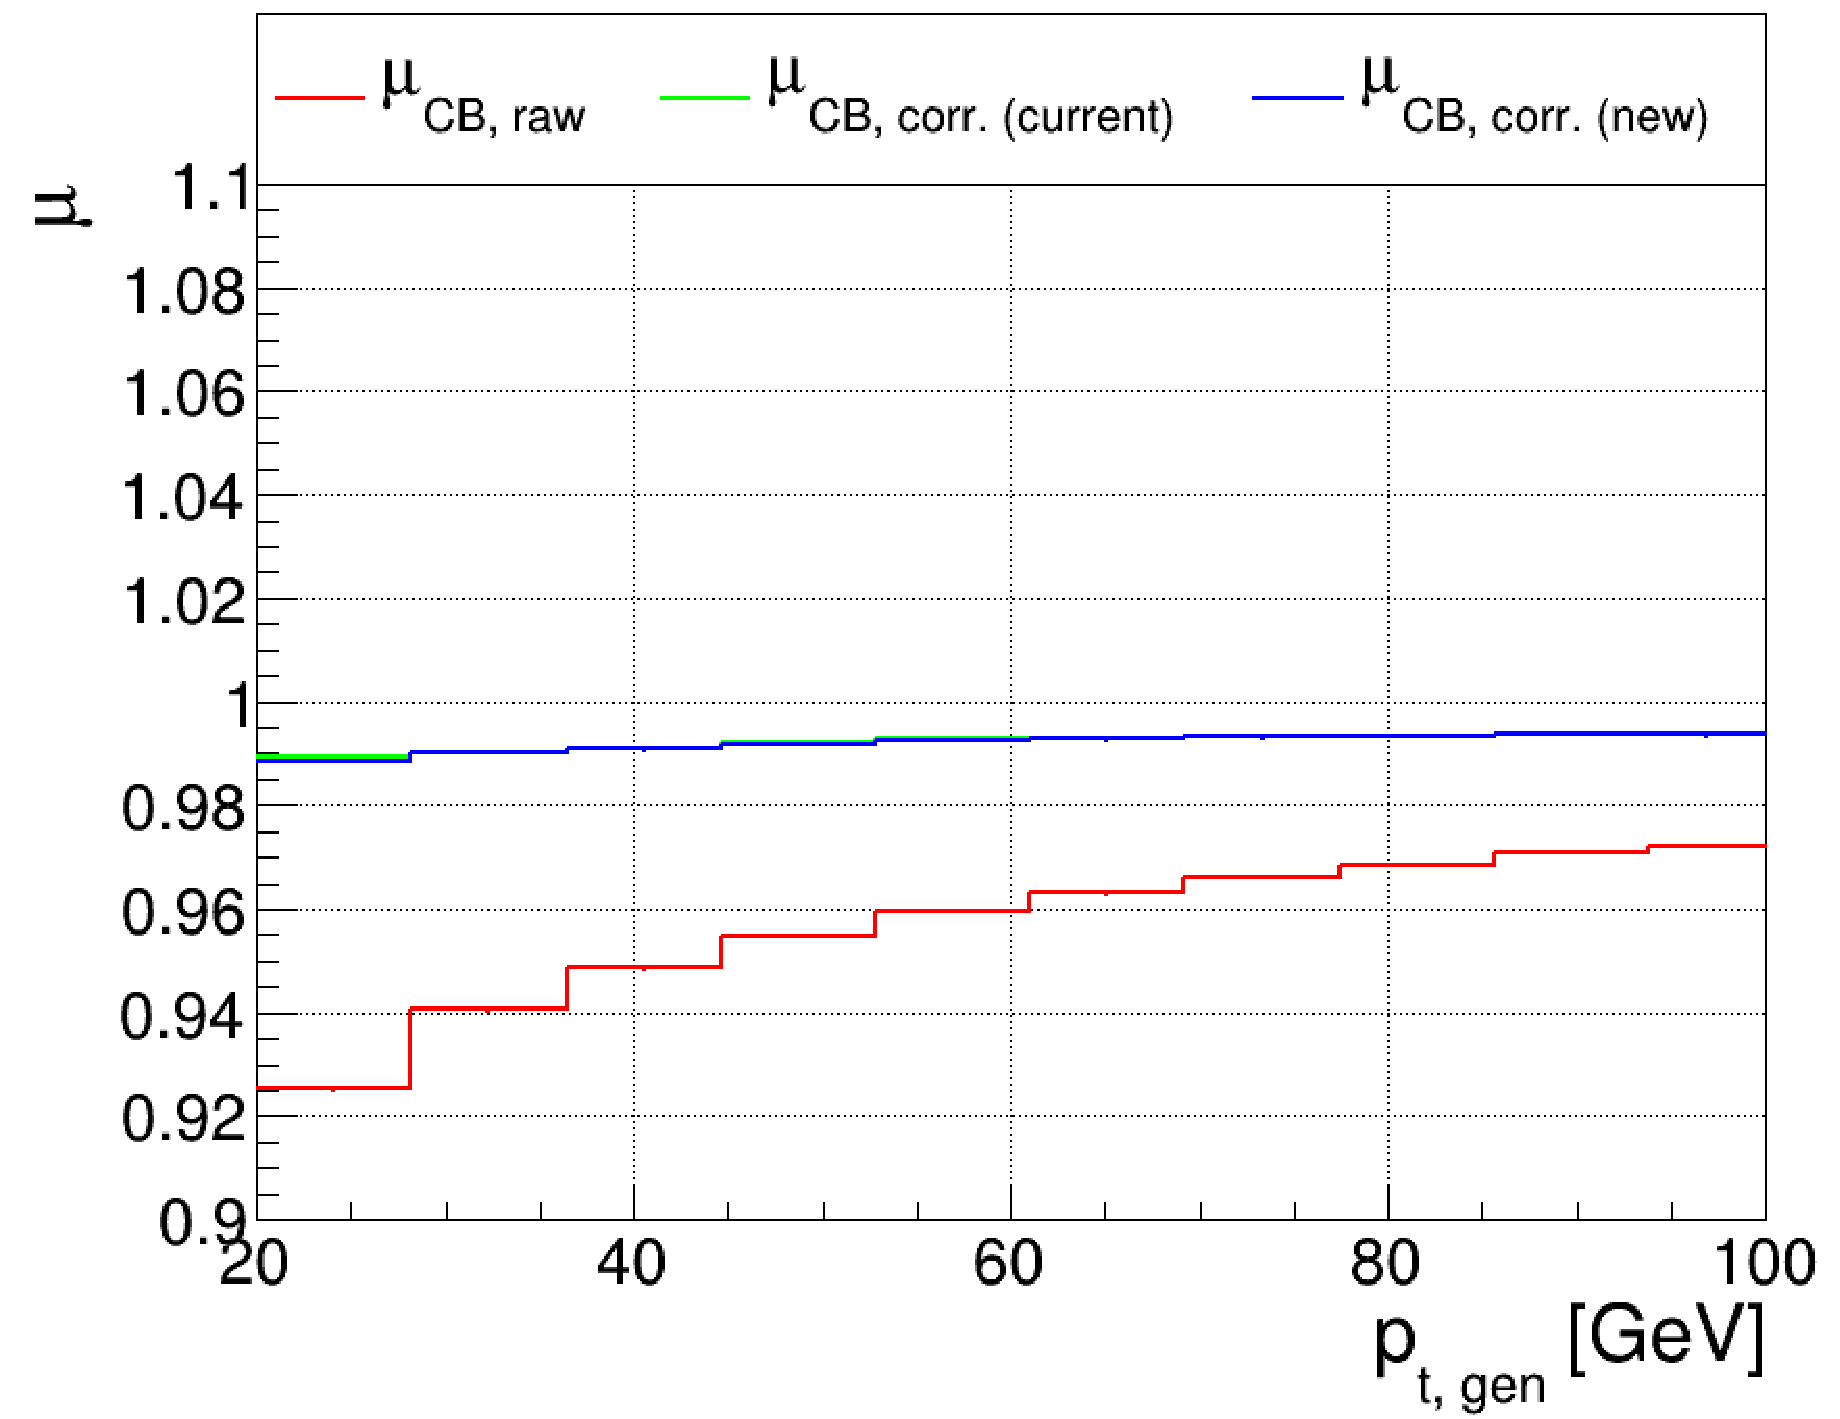
\includegraphics[width=0.495\textwidth]{./plots_pdf/ECAL_plots/plotsPU/EB/FULL/pdf/GENPT/EBFULL_GENPT_0020_0100_MuOverBins.pdf}
\includegraphics[width=0.495\textwidth]{./plots_pdf/ECAL_plots/plotsPU/EB/FULL/pdf/GENPT/EBFULL_GENPT_0020_0100_EffSigmaOverBins.pdf}
%\caption{EB - Full Readout pt 20-100}
%\end{figure}
%\begin{figure}
\includegraphics[width=0.495\textwidth]{./plots_pdf/ECAL_plots/plotsPU/EB/FULL/pdf/GENETA/EBFULL_GENETA_0020_0100_MuOverBins.pdf}
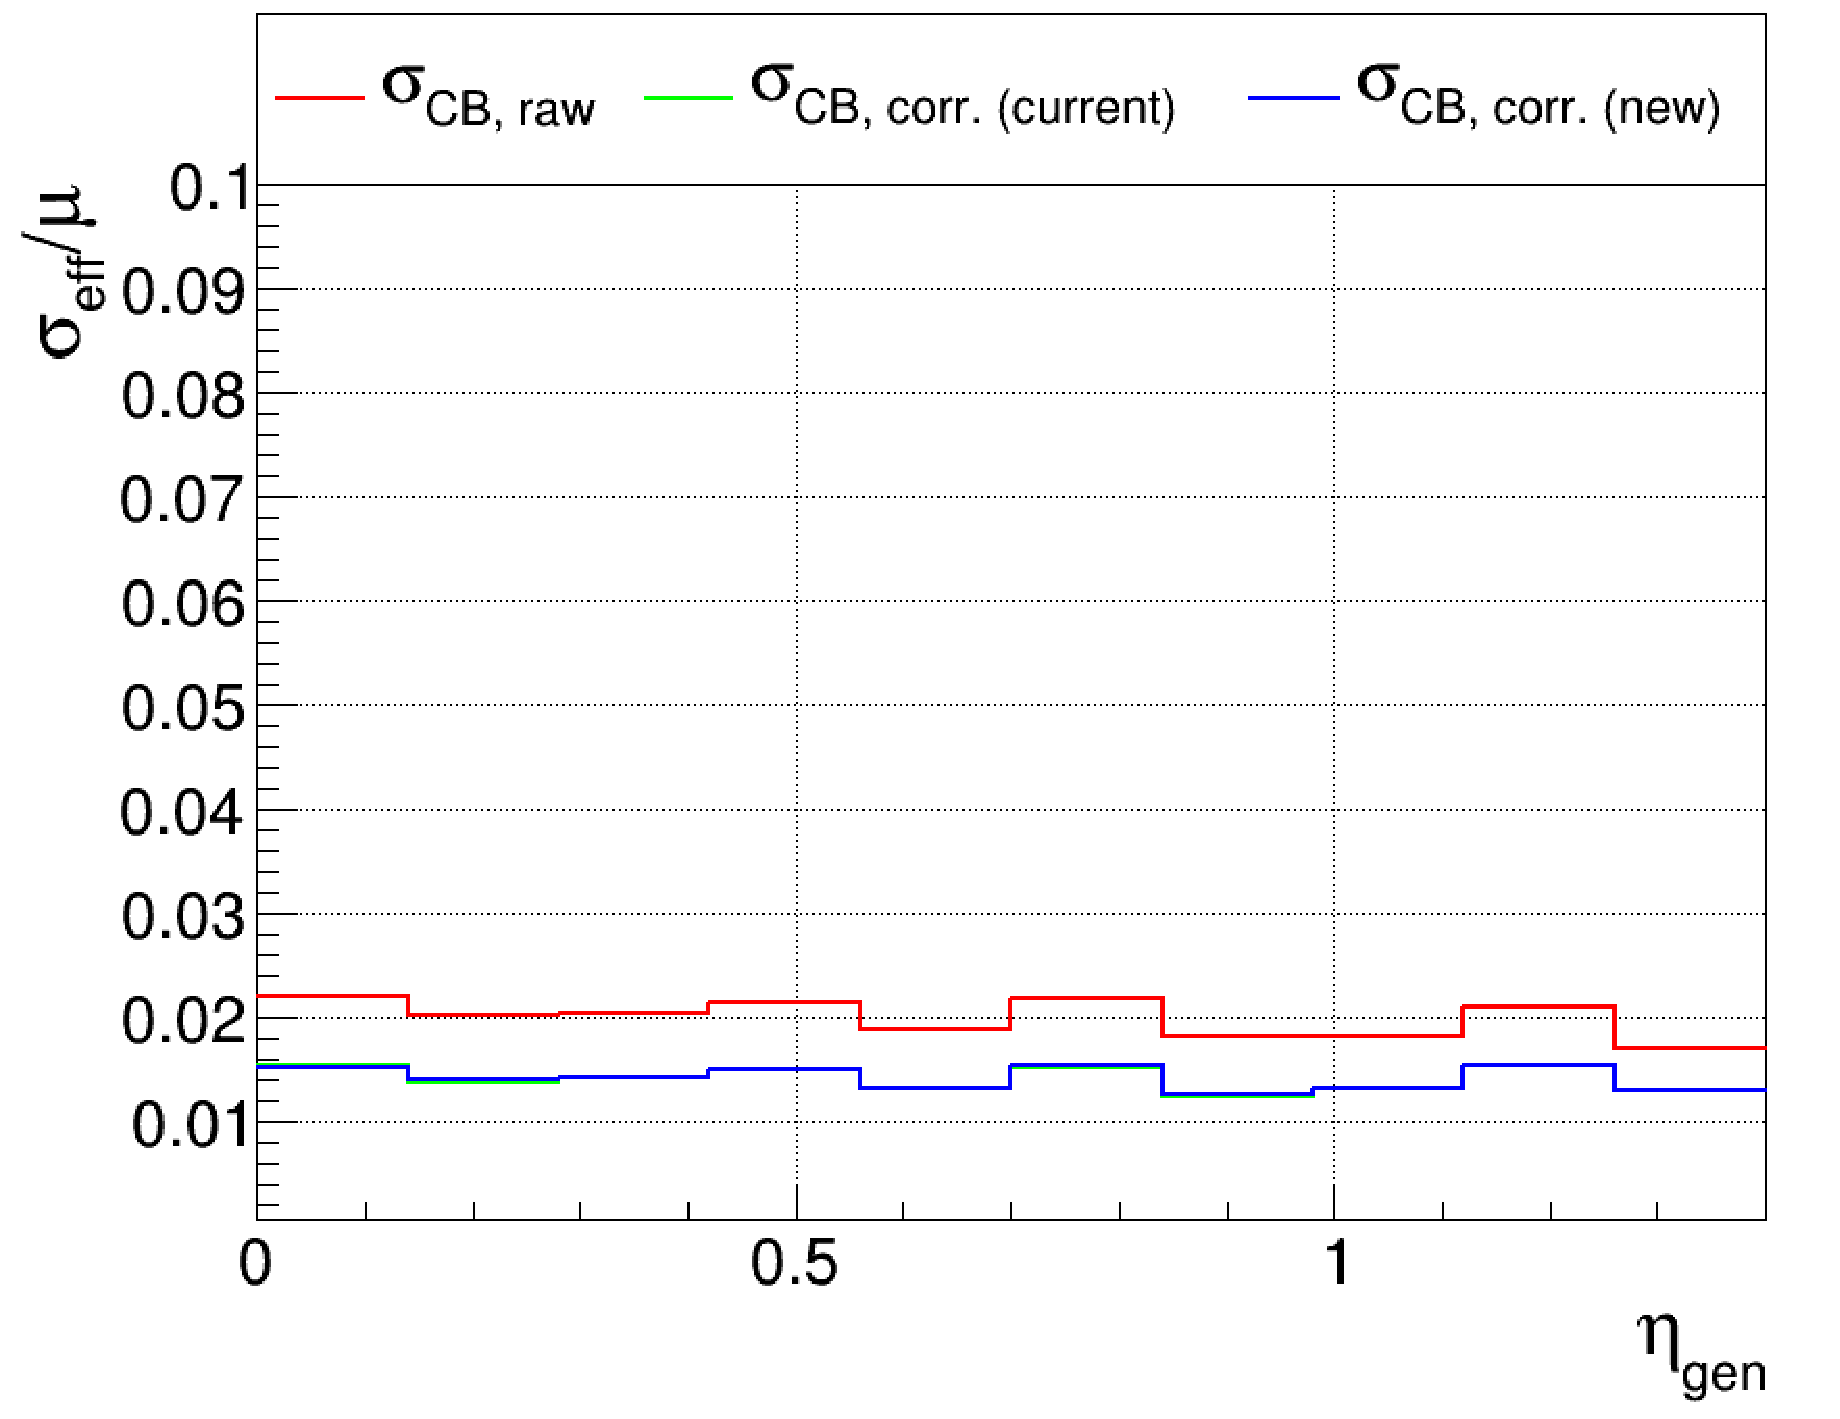
\includegraphics[width=0.495\textwidth]{./plots_pdf/ECAL_plots/plotsPU/EB/FULL/pdf/GENETA/EBFULL_GENETA_0020_0100_EffSigmaOverBins.pdf}
\caption{EB - Full Readout \pt 20--100\GeV.}
\end{figure}

\begin{figure}
\includegraphics[width=0.495\textwidth]{./plots_pdf/ECAL_plots/plotsPU/EB/FULL/pdf/GENPT/EBFULL_GENPT_0100_0300_MuOverBins.pdf}
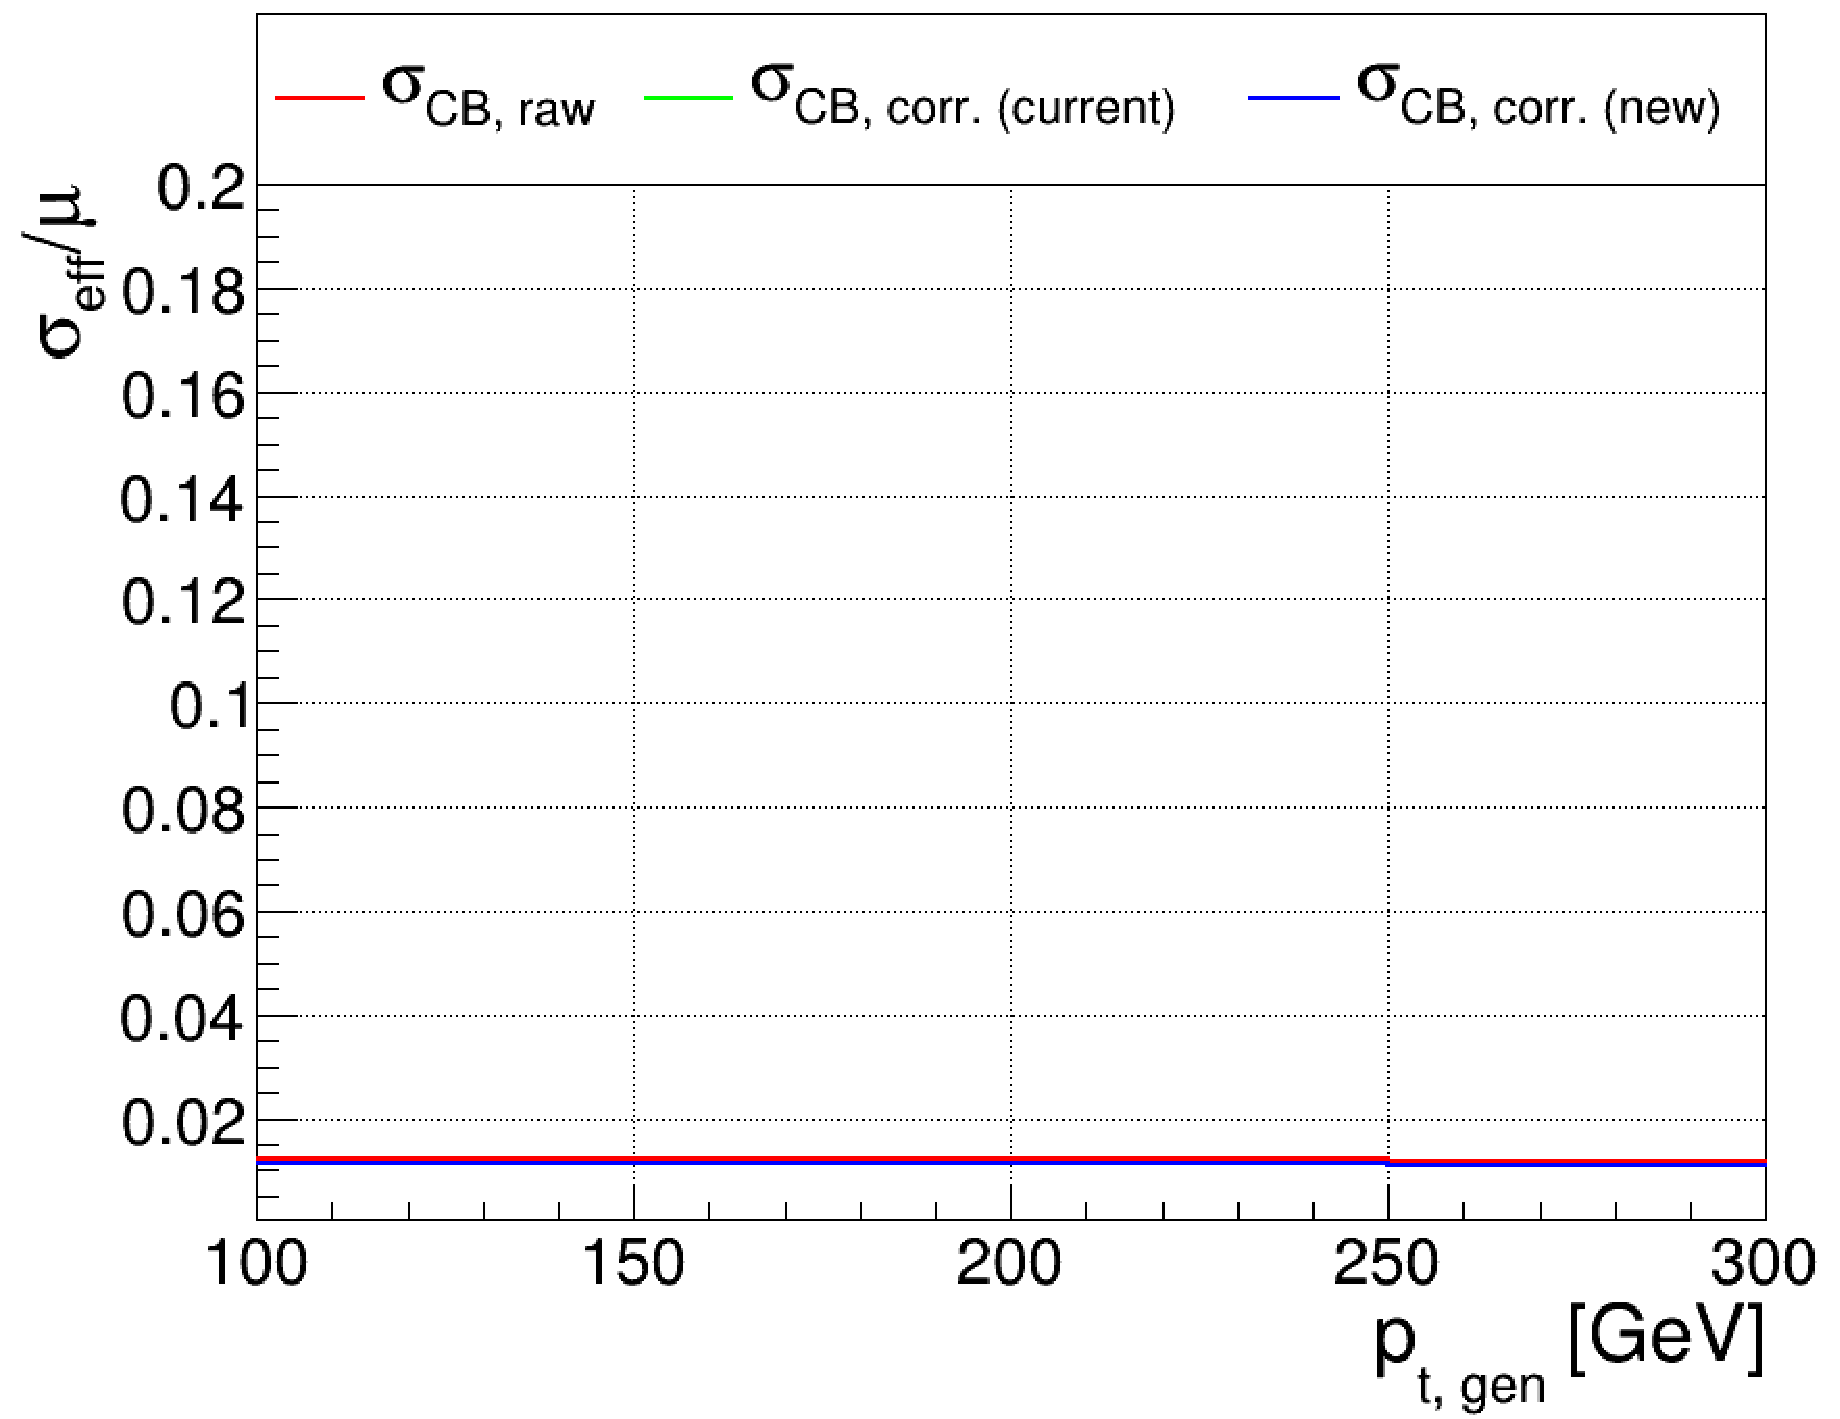
\includegraphics[width=0.495\textwidth]{./plots_pdf/ECAL_plots/plotsPU/EB/FULL/pdf/GENPT/EBFULL_GENPT_0100_0300_EffSigmaOverBins.pdf}
%\caption{EB - Full Readout pt 100-300}
%\end{figure}
%\begin{figure}
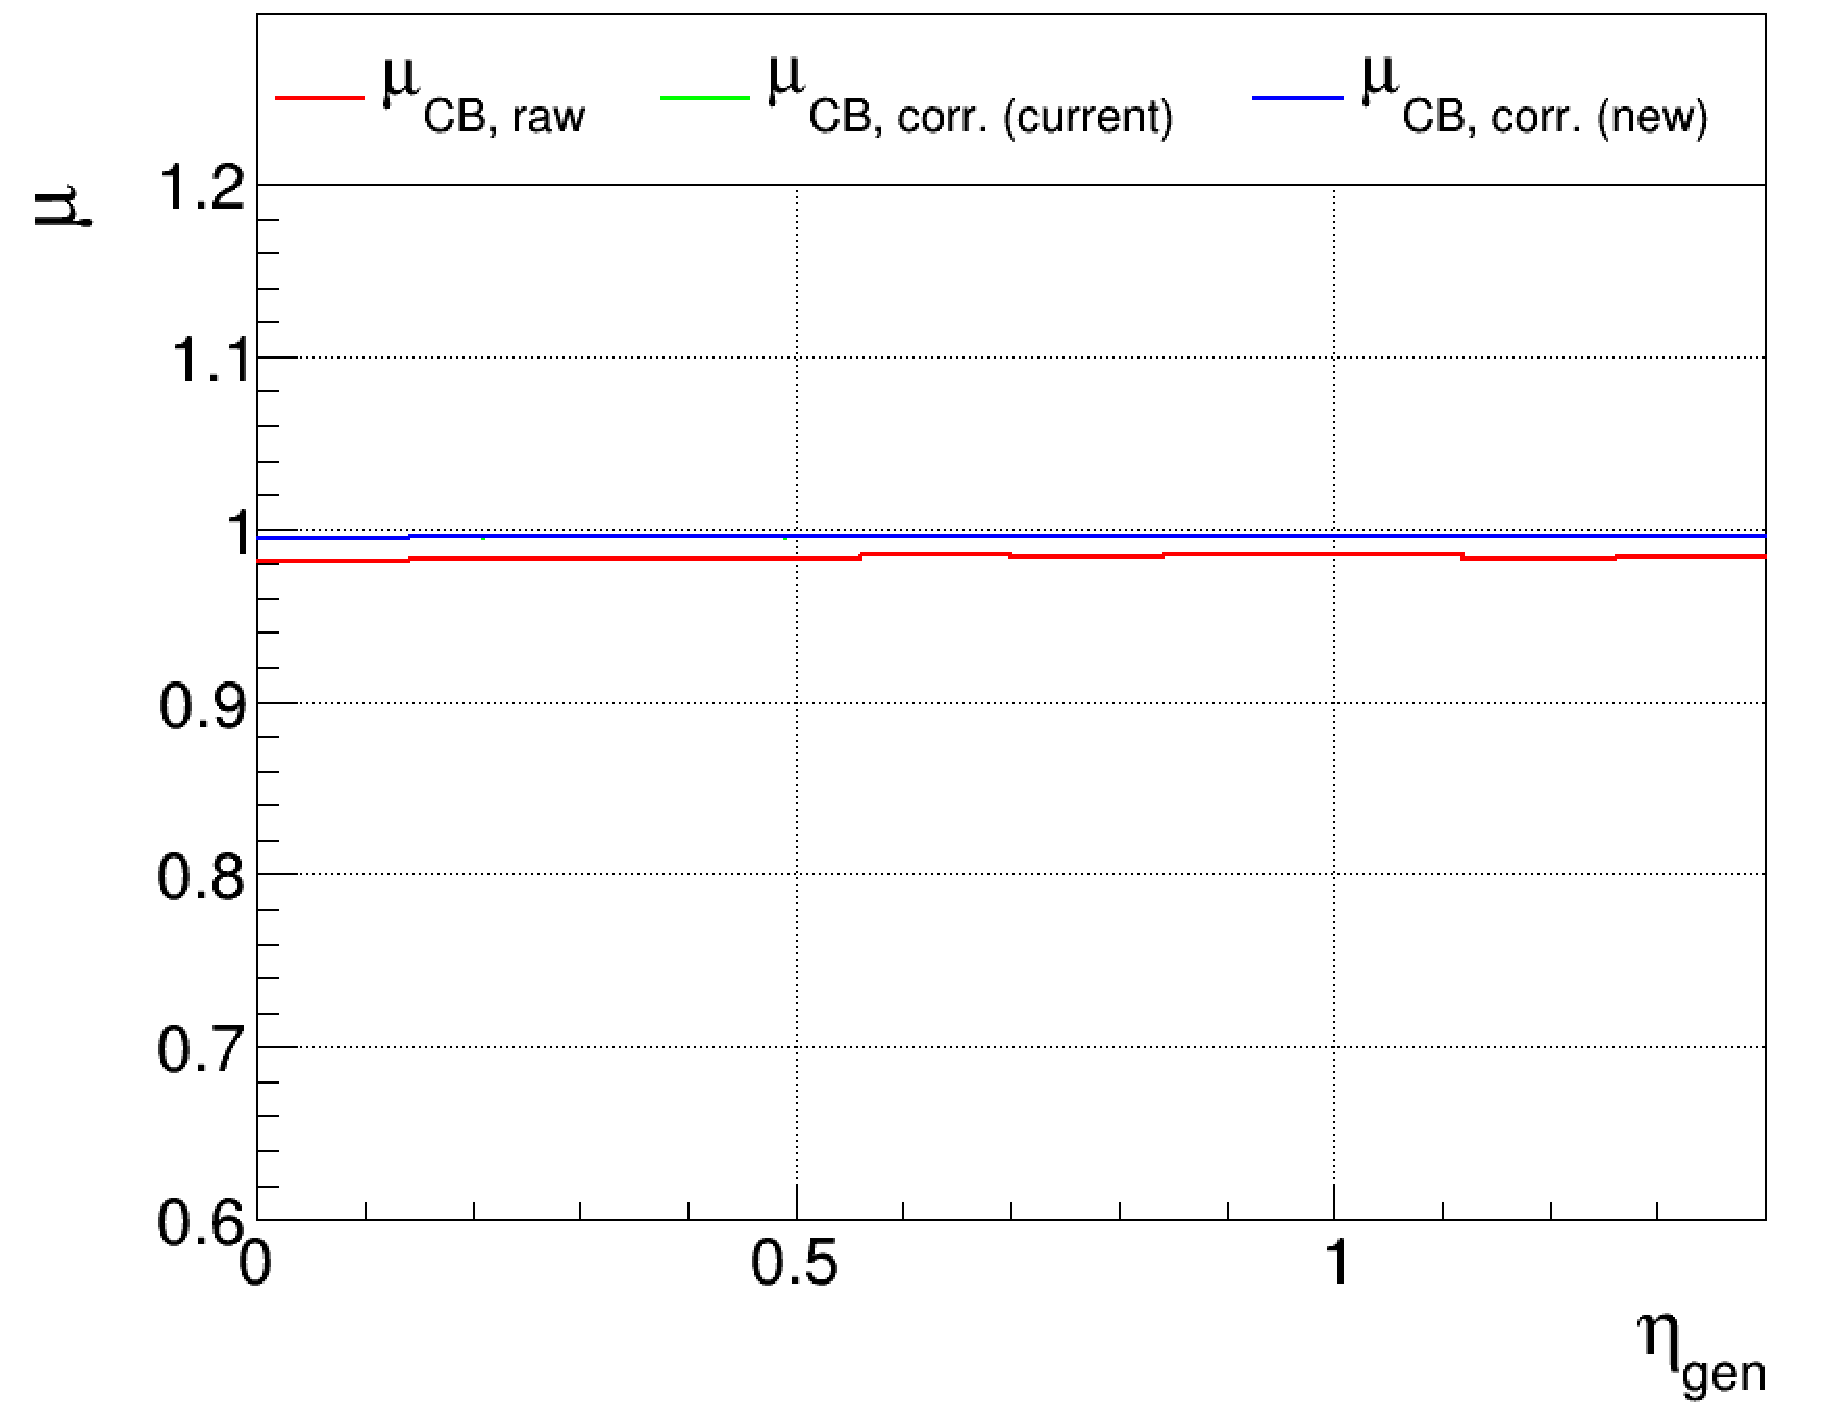
\includegraphics[width=0.495\textwidth]{./plots_pdf/ECAL_plots/plotsPU/EB/FULL/pdf/GENETA/EBFULL_GENETA_0100_0300_MuOverBins.pdf}
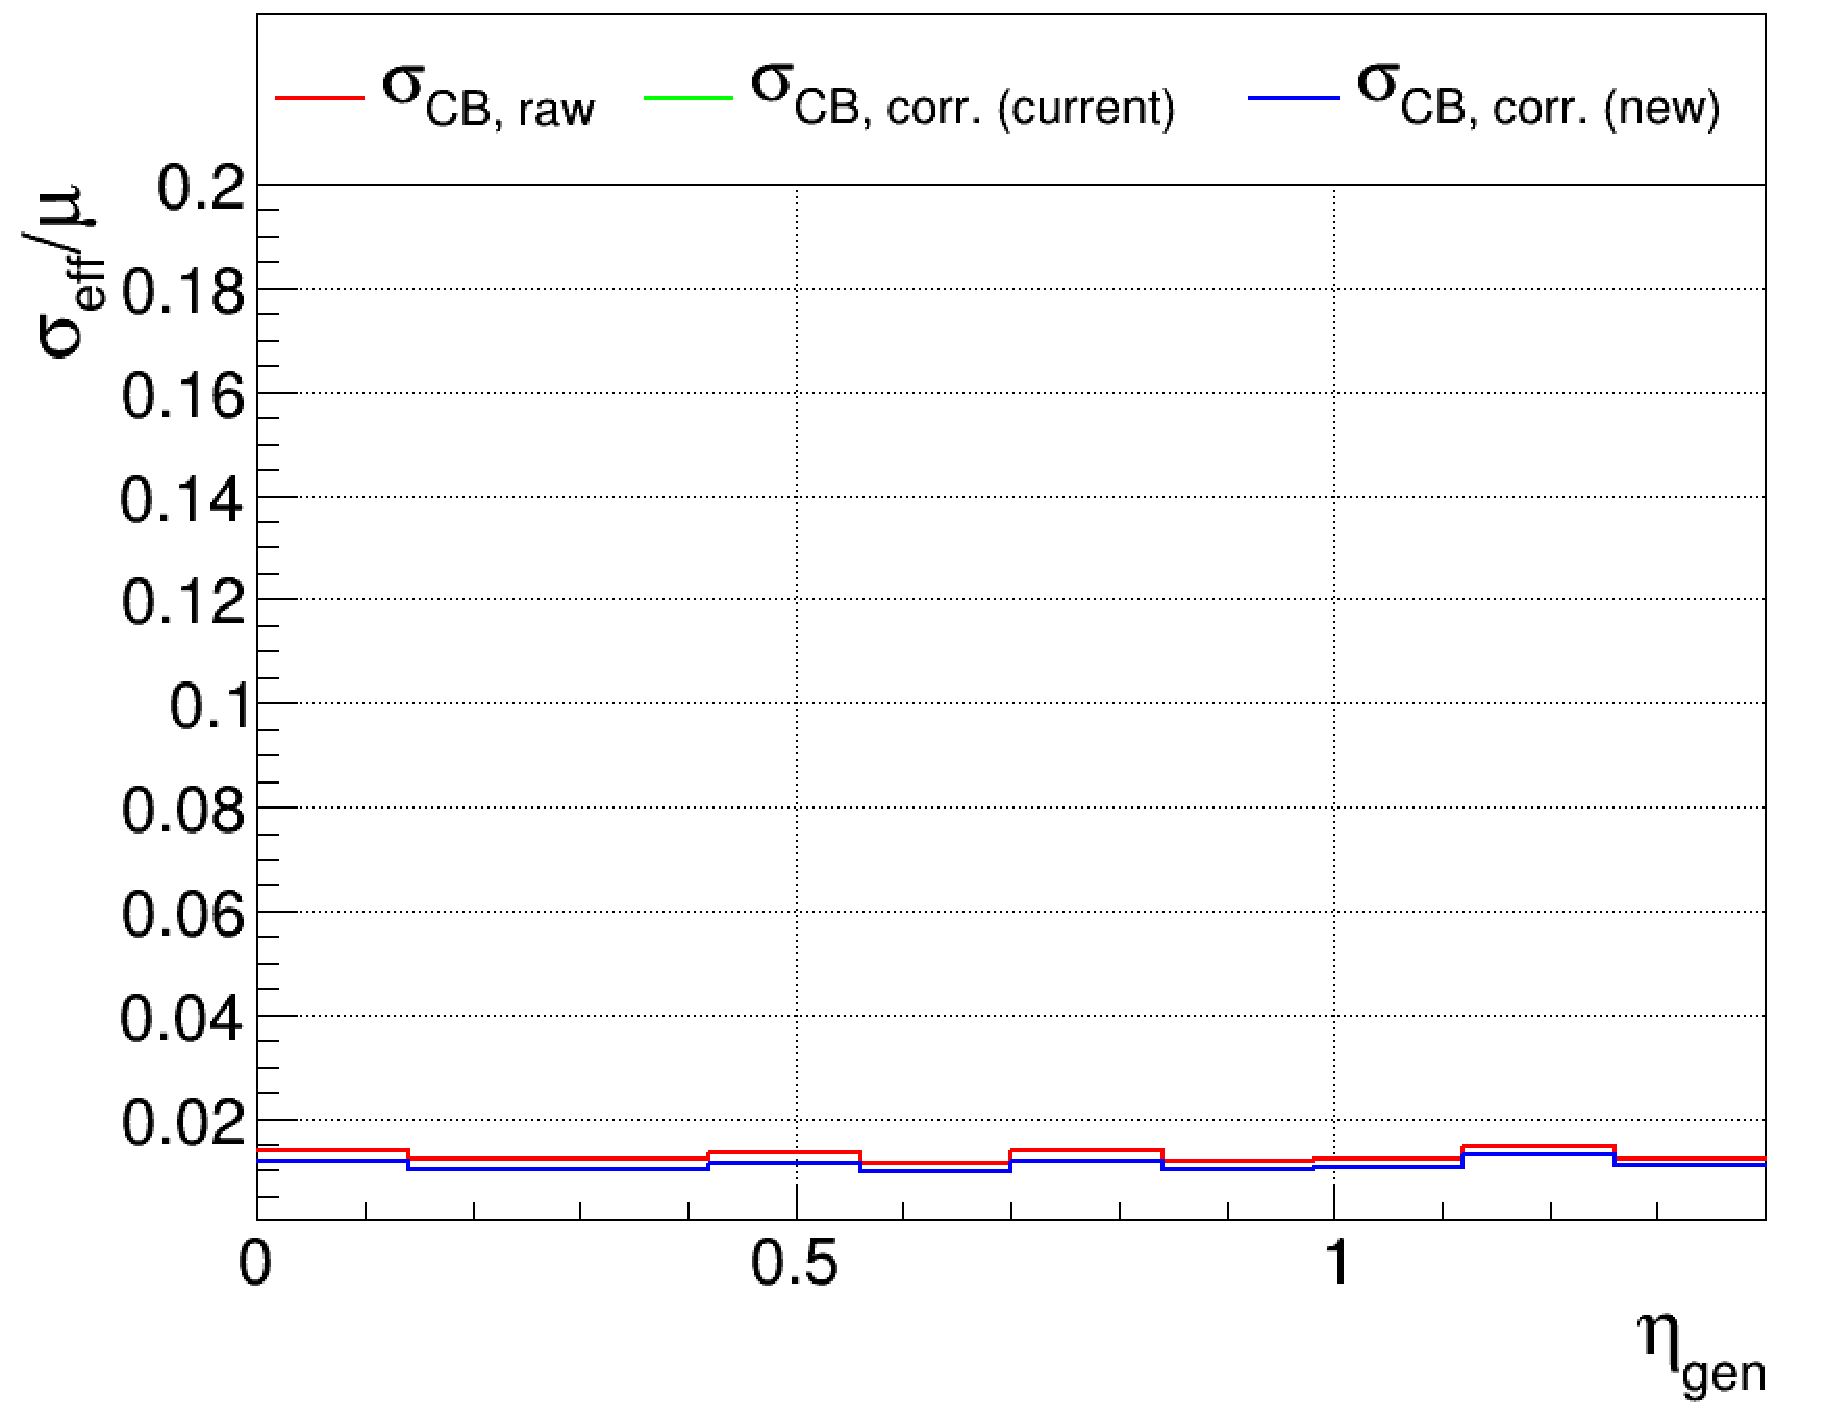
\includegraphics[width=0.495\textwidth]{./plots_pdf/ECAL_plots/plotsPU/EB/FULL/pdf/GENETA/EBFULL_GENETA_0100_0300_EffSigmaOverBins.pdf}
\caption{EB - Full Readout \pt 100-300\GeV}
\end{figure}





\begin{figure}
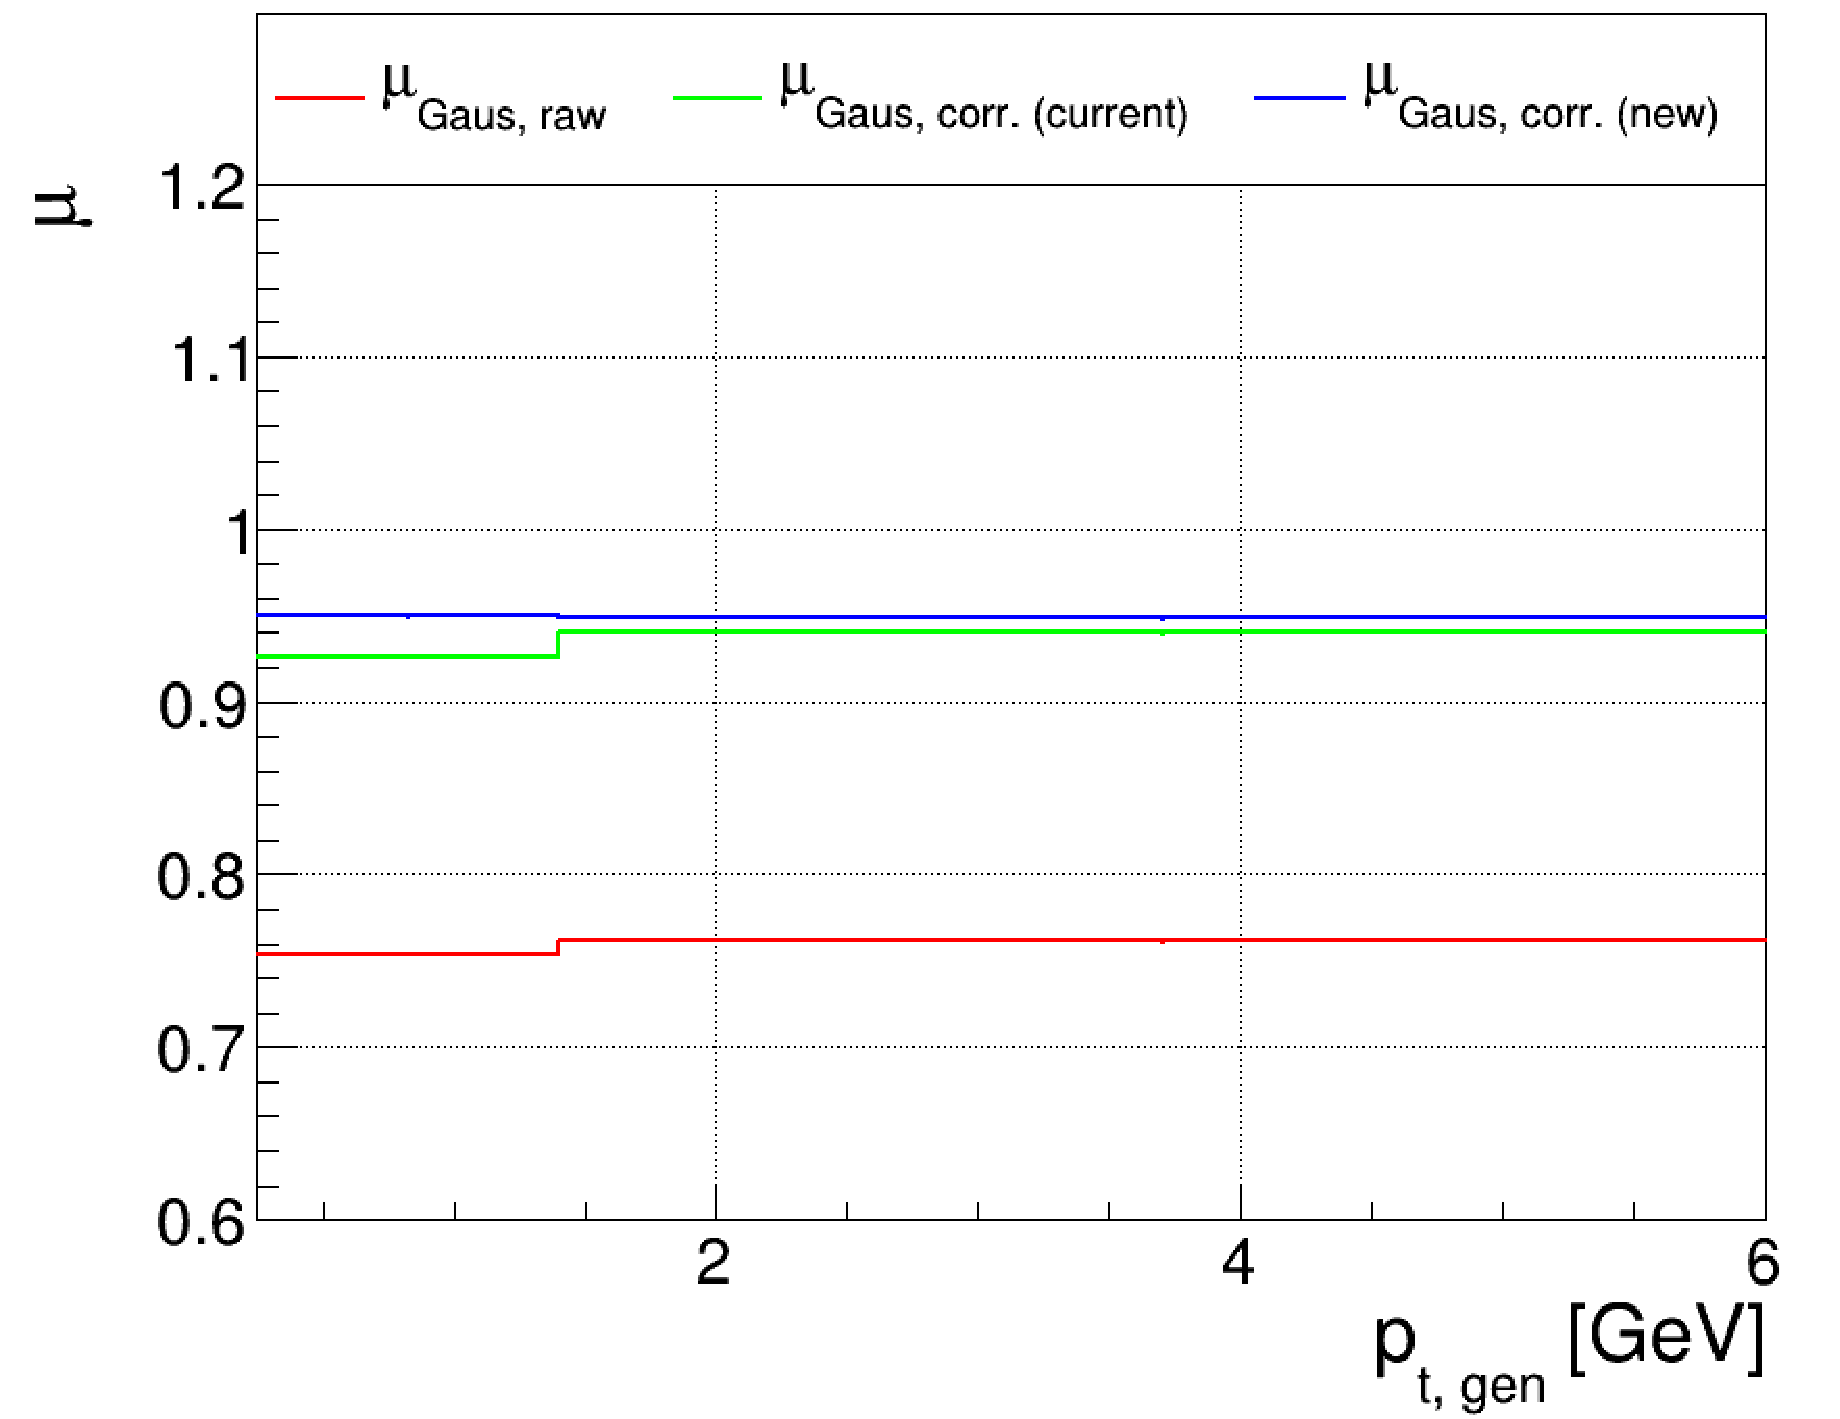
\includegraphics[width=0.495\textwidth]{./plots_pdf/ECAL_plots/plotsPU/EB/ZS/pdf/GENPT/EBZS_GENPT_0000_0006_MuOverBins.pdf}
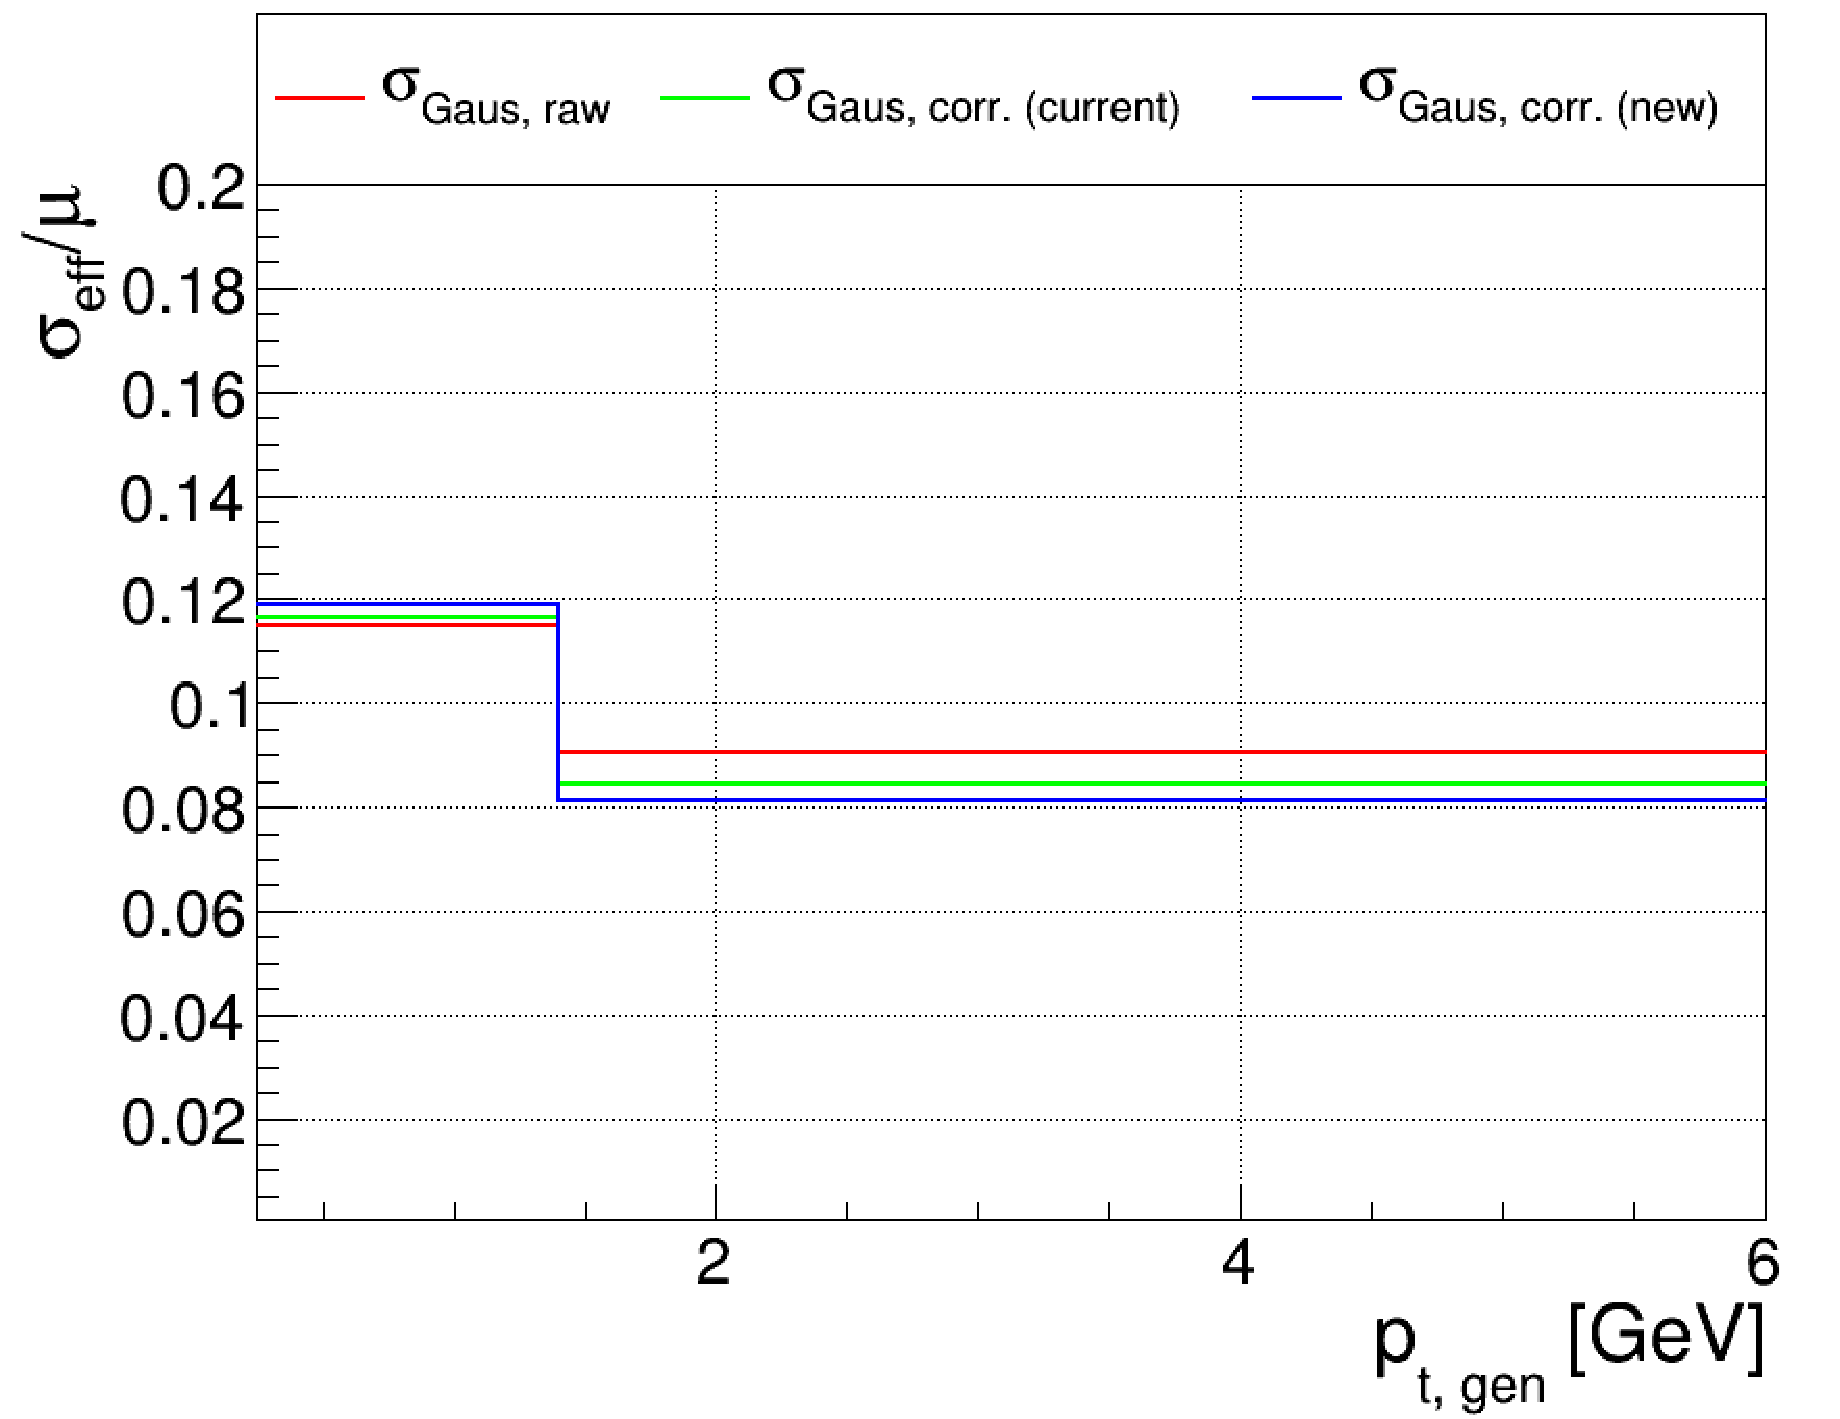
\includegraphics[width=0.495\textwidth]{./plots_pdf/ECAL_plots/plotsPU/EB/ZS/pdf/GENPT/EBZS_GENPT_0000_0006_EffSigmaOverBins.pdf}

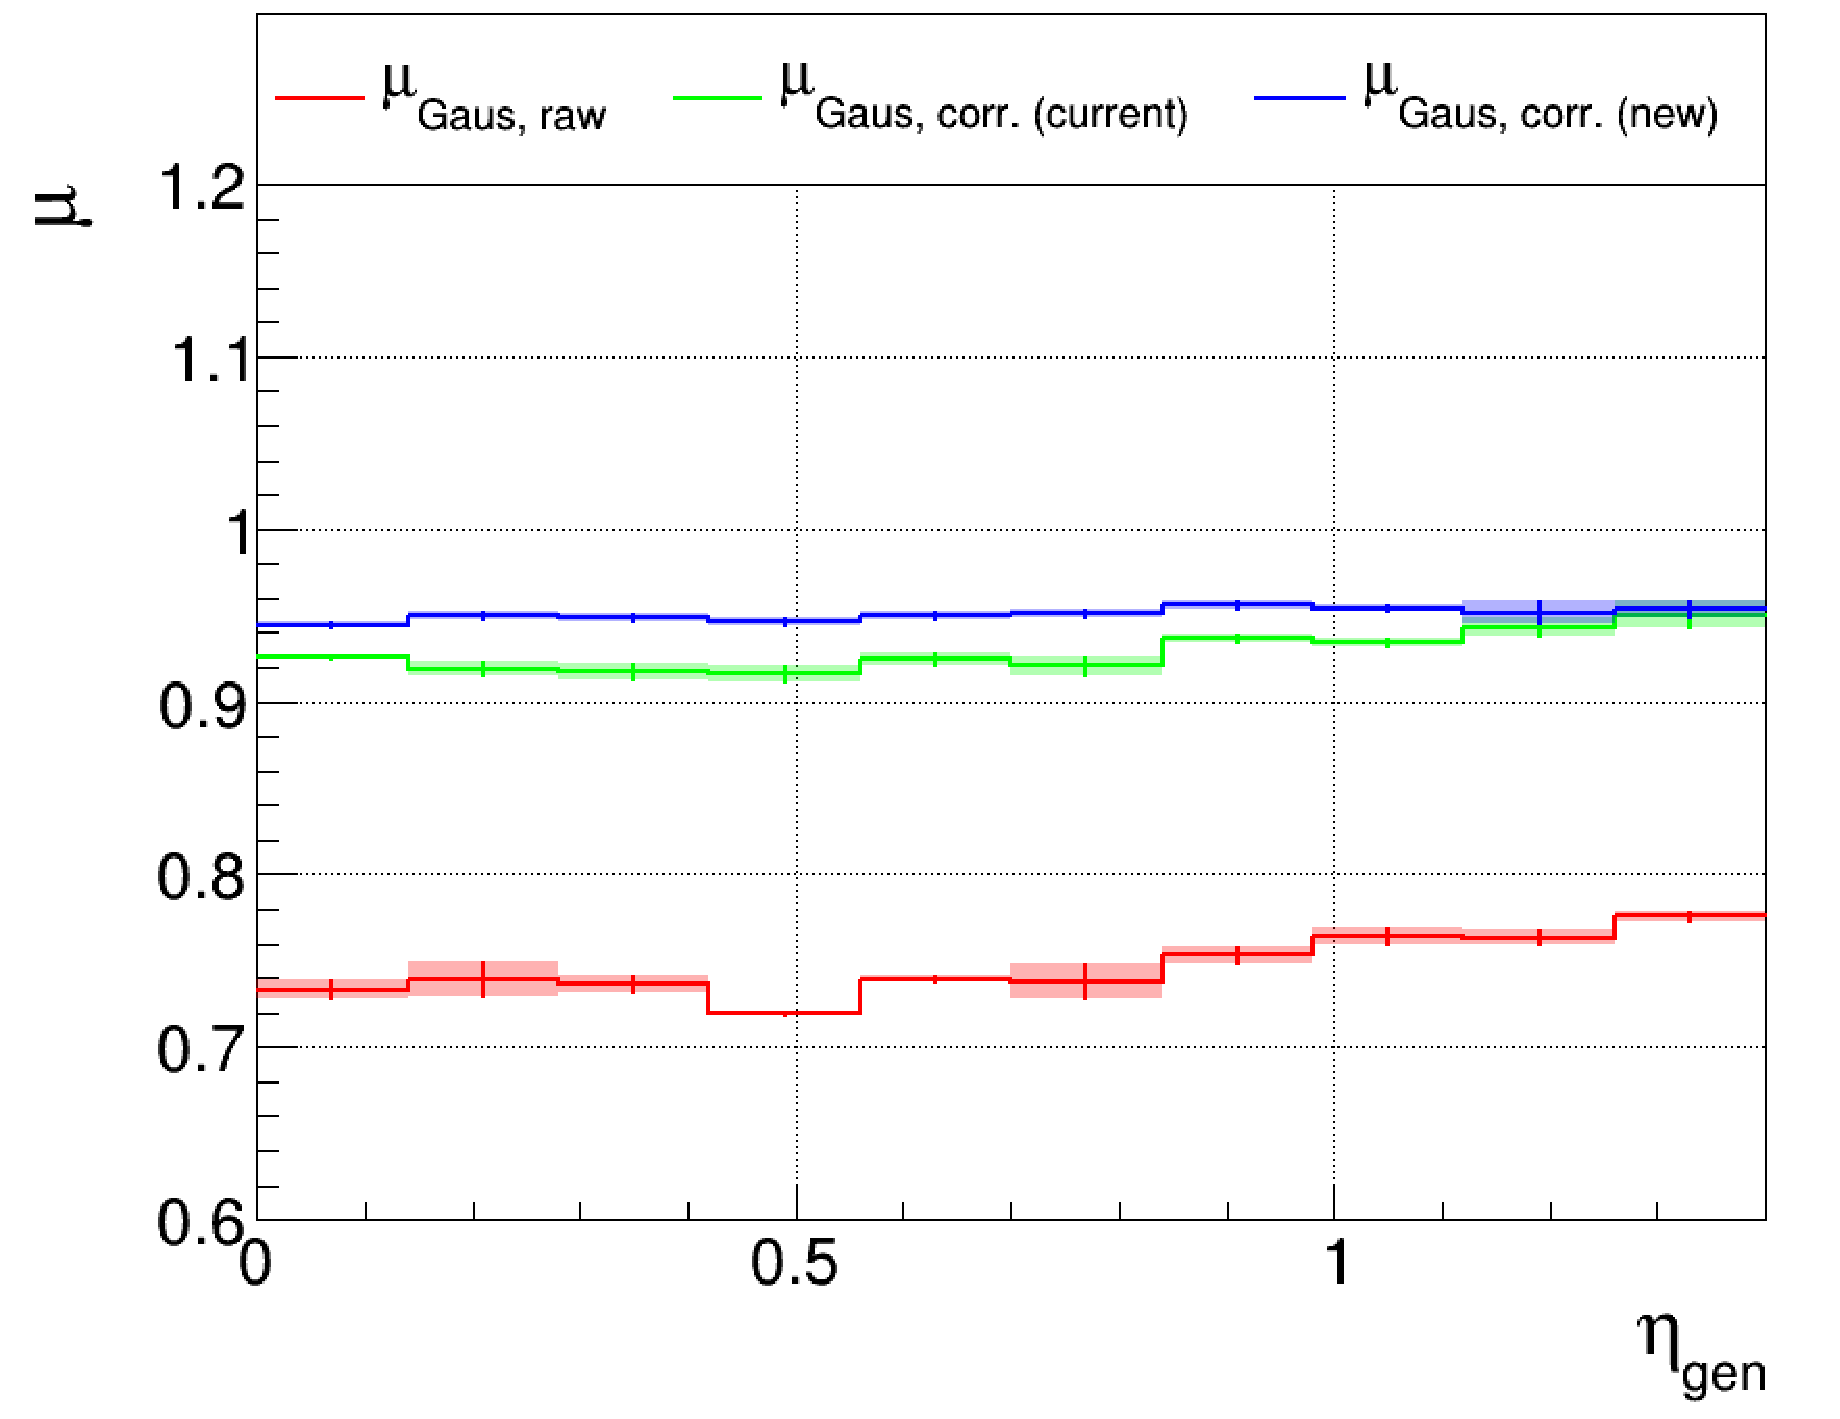
\includegraphics[width=0.495\textwidth]{./plots_pdf/ECAL_plots/plotsPU/EB/ZS/pdf/GENETA/EBZS_GENETA_0000_0006_MuOverBins.pdf}
\includegraphics[width=0.495\textwidth]{./plots_pdf/ECAL_plots/plotsPU/EB/ZS/pdf/GENETA/EBZS_GENETA_0000_0006_EffSigmaOverBins.pdf}
\caption[$\mu$ ($\sigma_\mathrm{eff}$) vs \pt of PF ECAL cluster - EB ZS readout PU  senario]{Mean response (resolution) defined by Raw PF ECAL clusters (red), the calibration derived earlier in Ru\
n3 based on 126X (green), and the new correction from 2024 simulation sample based on 133X (blue). \pt 0--6\GeV PU EB ZS readout PU senario.}
\label{fig:PU_EBZS}
\end{figure}

%% %\begin{figure}
%% \includegraphics[width=0.495\textwidth]{./plots_pdf/ECAL_plots/plotsPU/EB/ZS/pdf/GENPT/EBZS_GENPT_0006_0025_MuOverBins.pdf}
%% 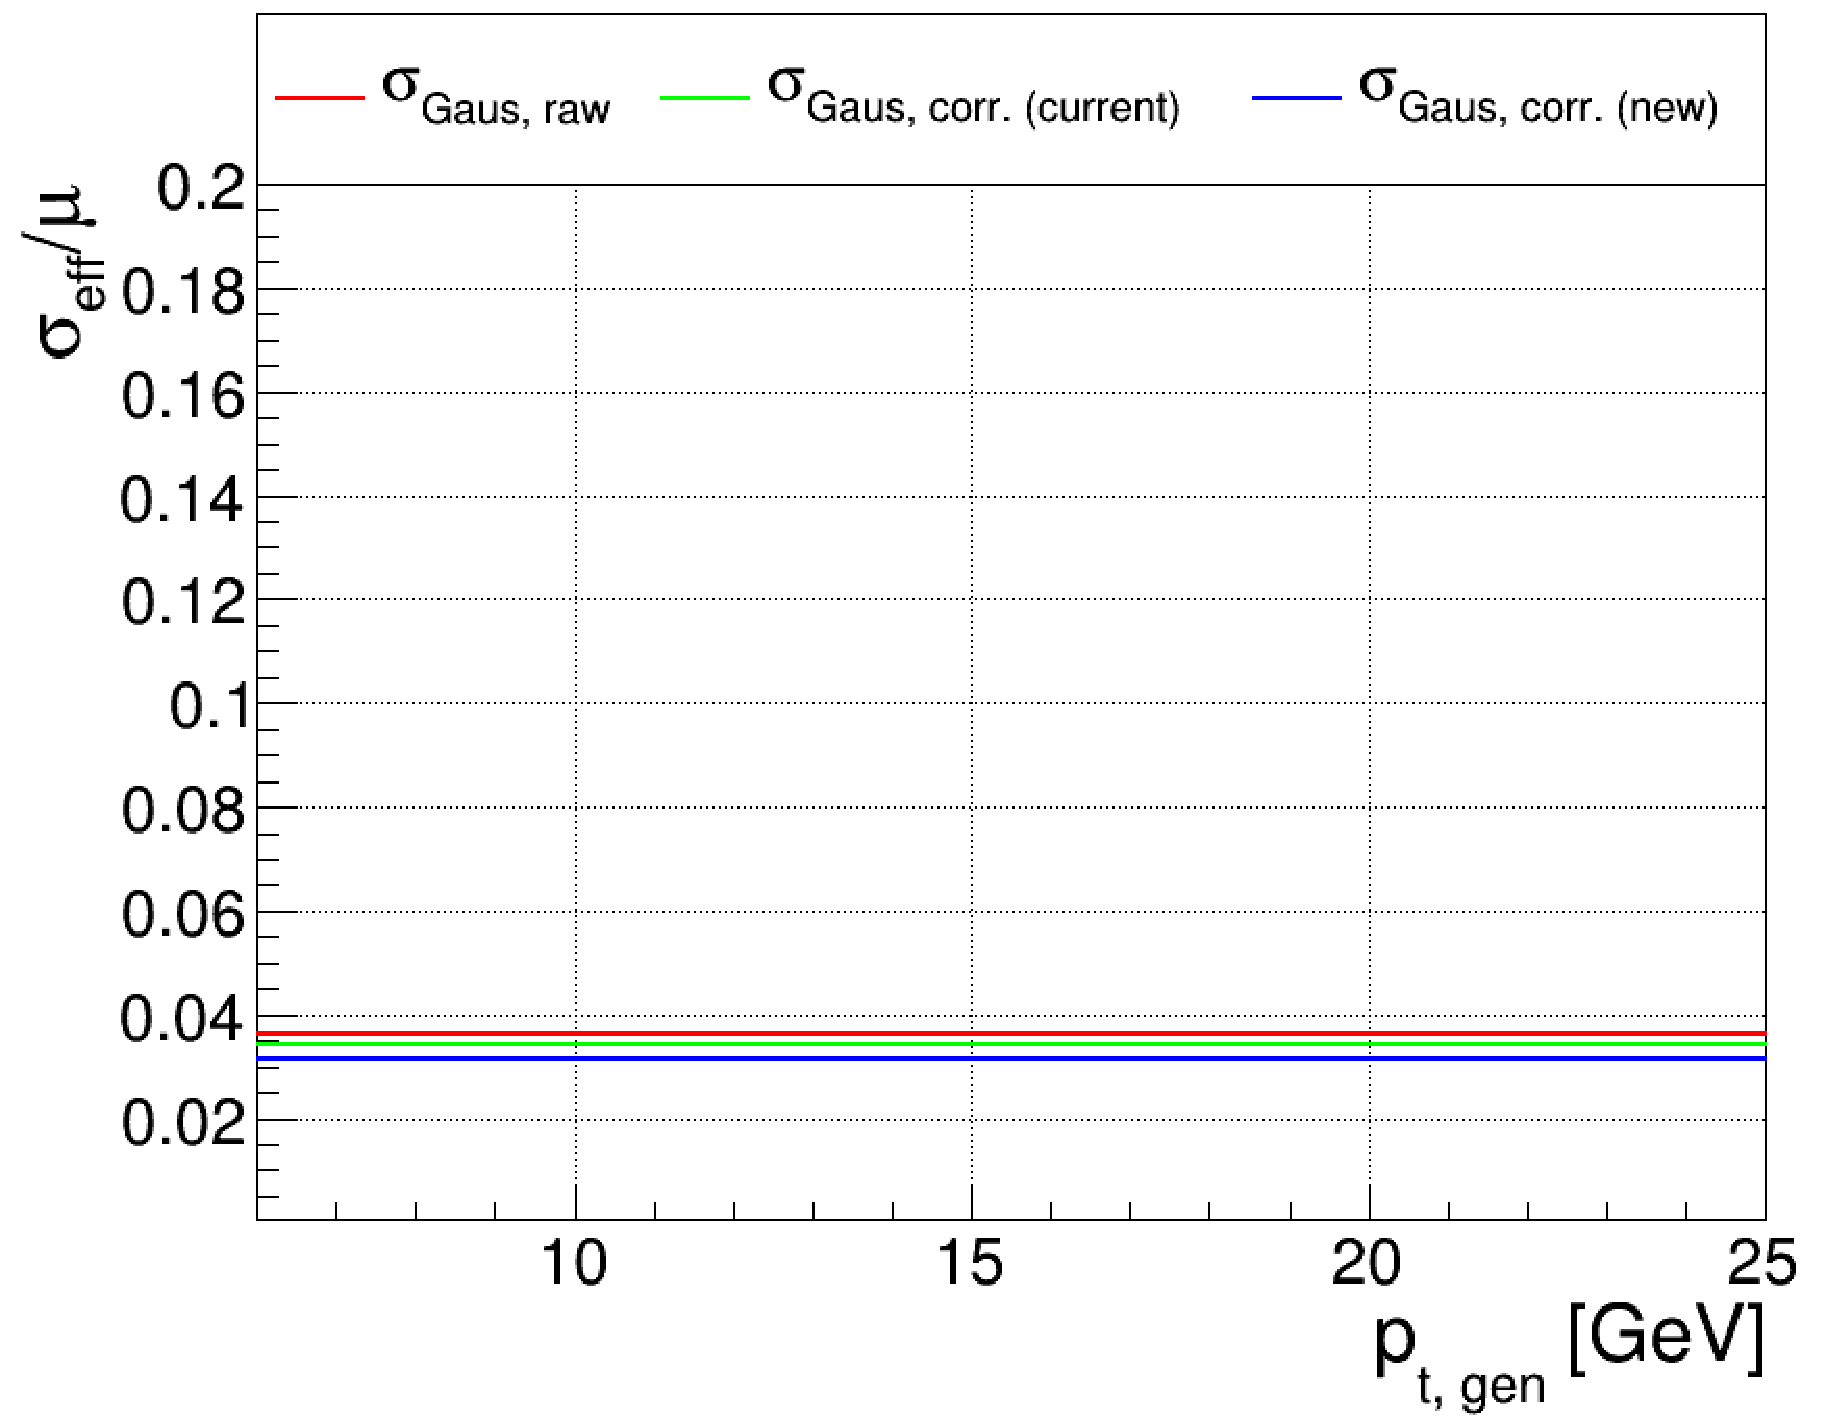
\includegraphics[width=0.495\textwidth]{./plots_pdf/ECAL_plots/plotsPU/EB/ZS/pdf/GENPT/EBZS_GENPT_0006_0025_EffSigmaOverBins.pdf}
%% %\caption{EB - ZS Readout pt 6-25}
%% %\end{figure}
%% %\begin{figure}
%% 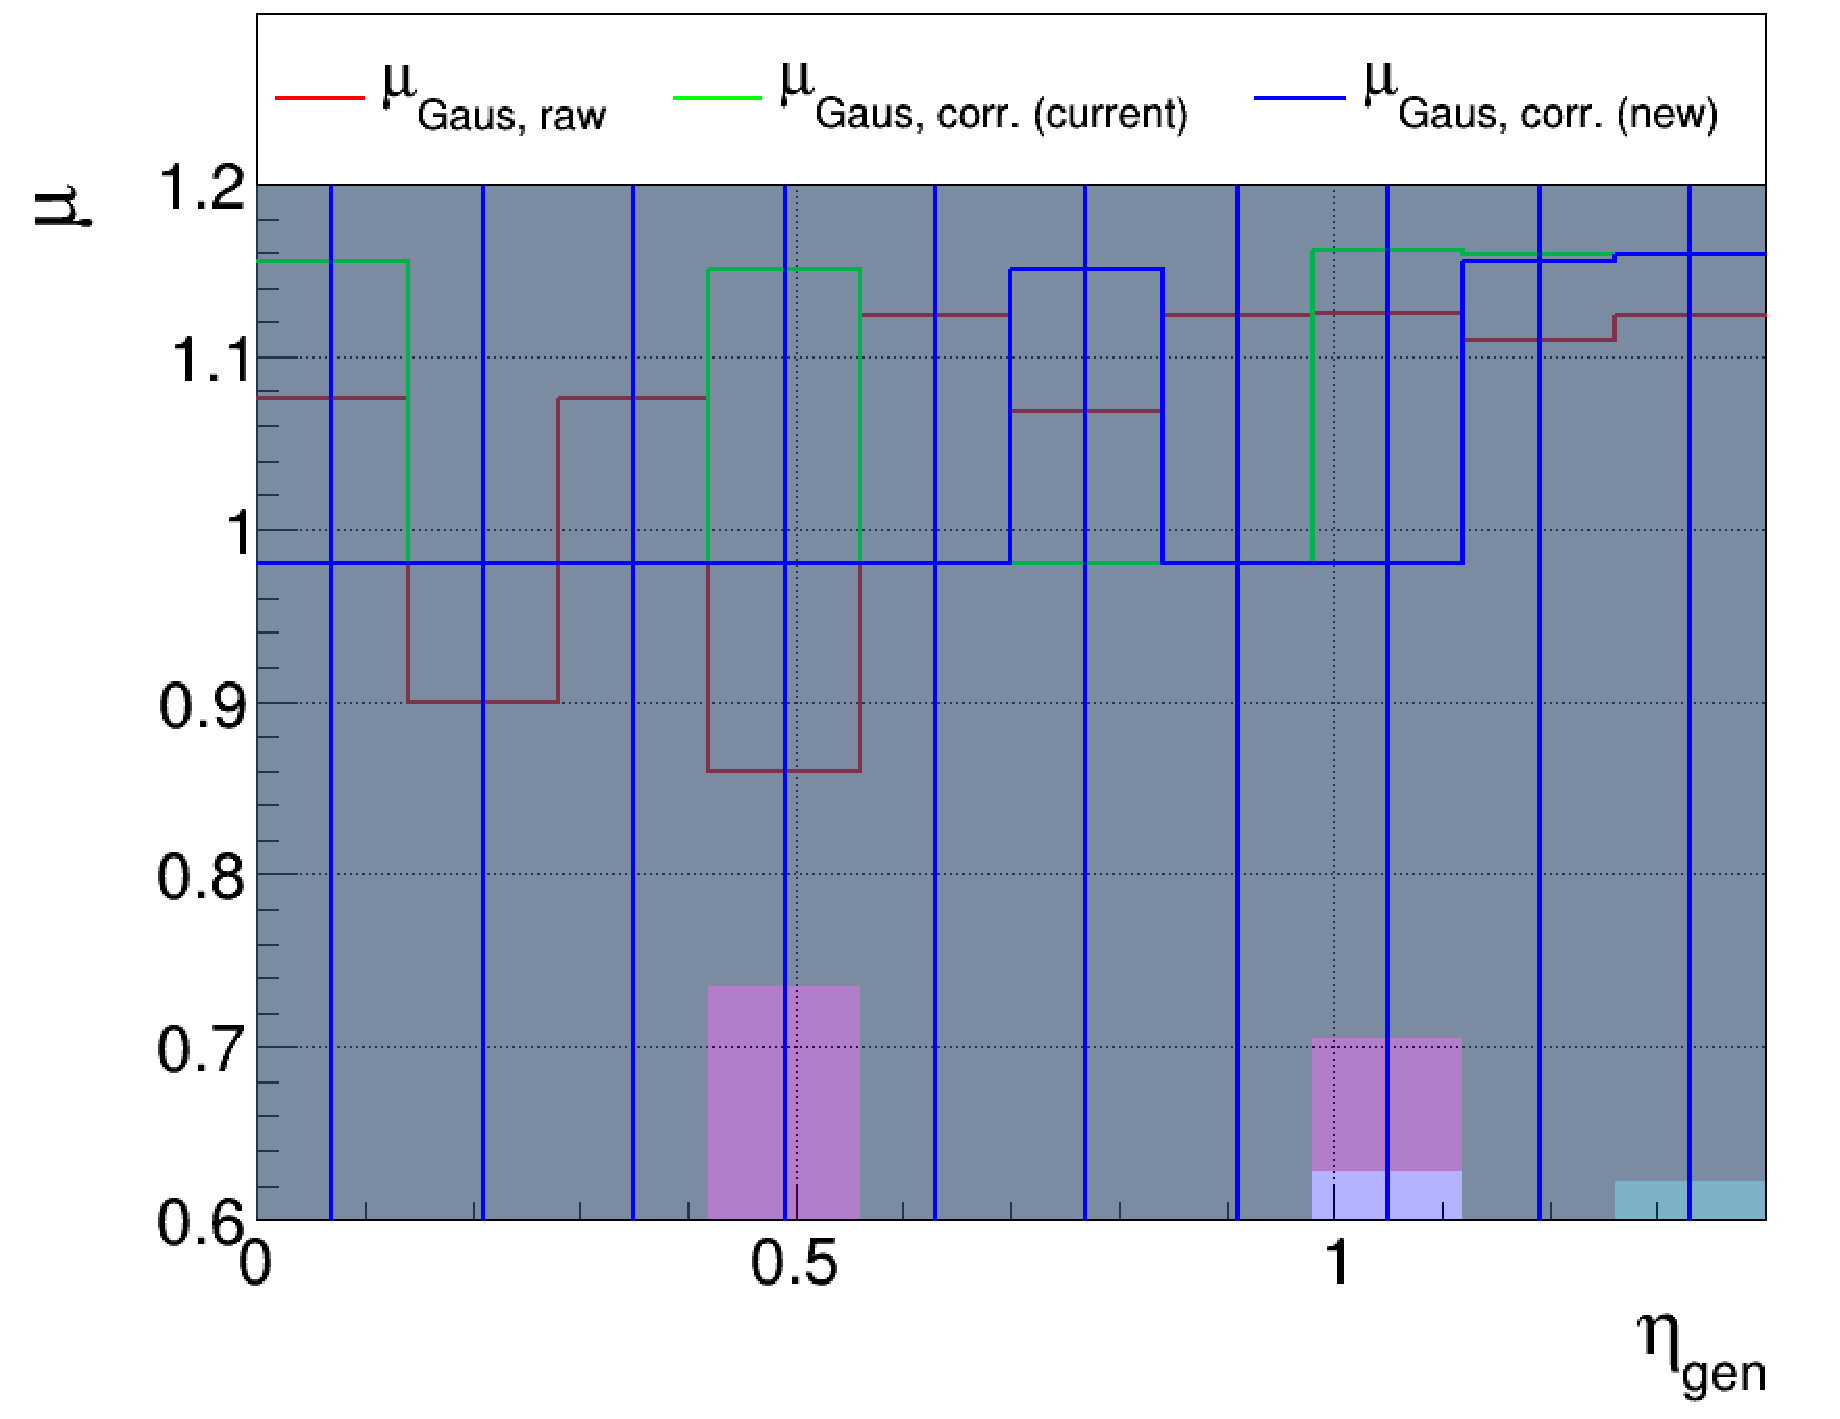
\includegraphics[width=0.495\textwidth]{./plots_pdf/ECAL_plots/plotsPU/EB/ZS/pdf/GENETA/EBZS_GENETA_0006_0025_MuOverBins.pdf}
%% 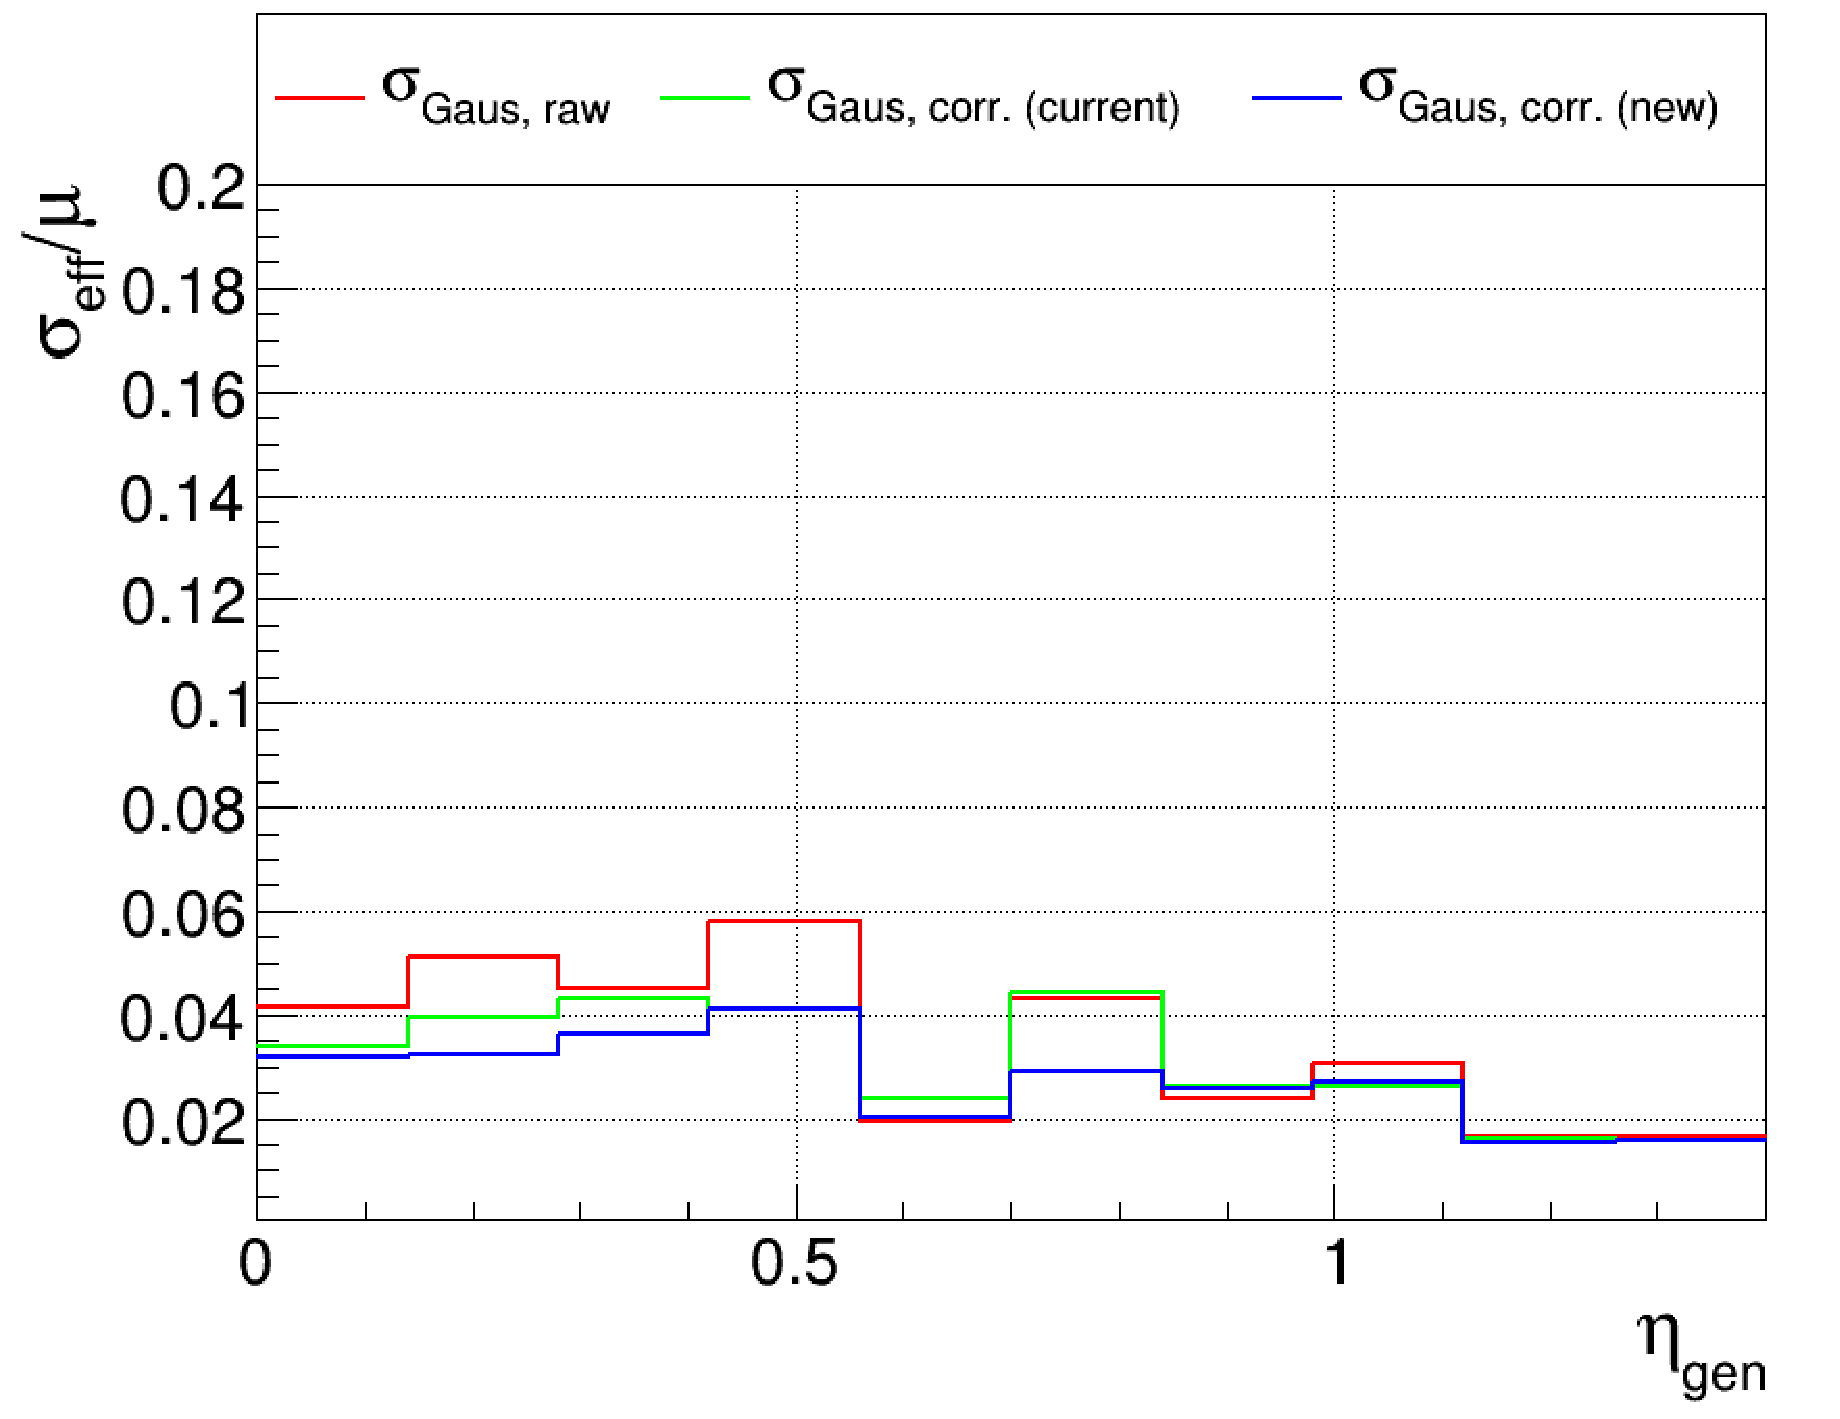
\includegraphics[width=0.495\textwidth]{./plots_pdf/ECAL_plots/plotsPU/EB/ZS/pdf/GENETA/EBZS_GENETA_0006_0025_EffSigmaOverBins.pdf}
%% \caption{EB - ZS Readout \pt 6-25}
%% \end{figure}







%\subsubsection{ECAL Endcap}

\begin{figure}
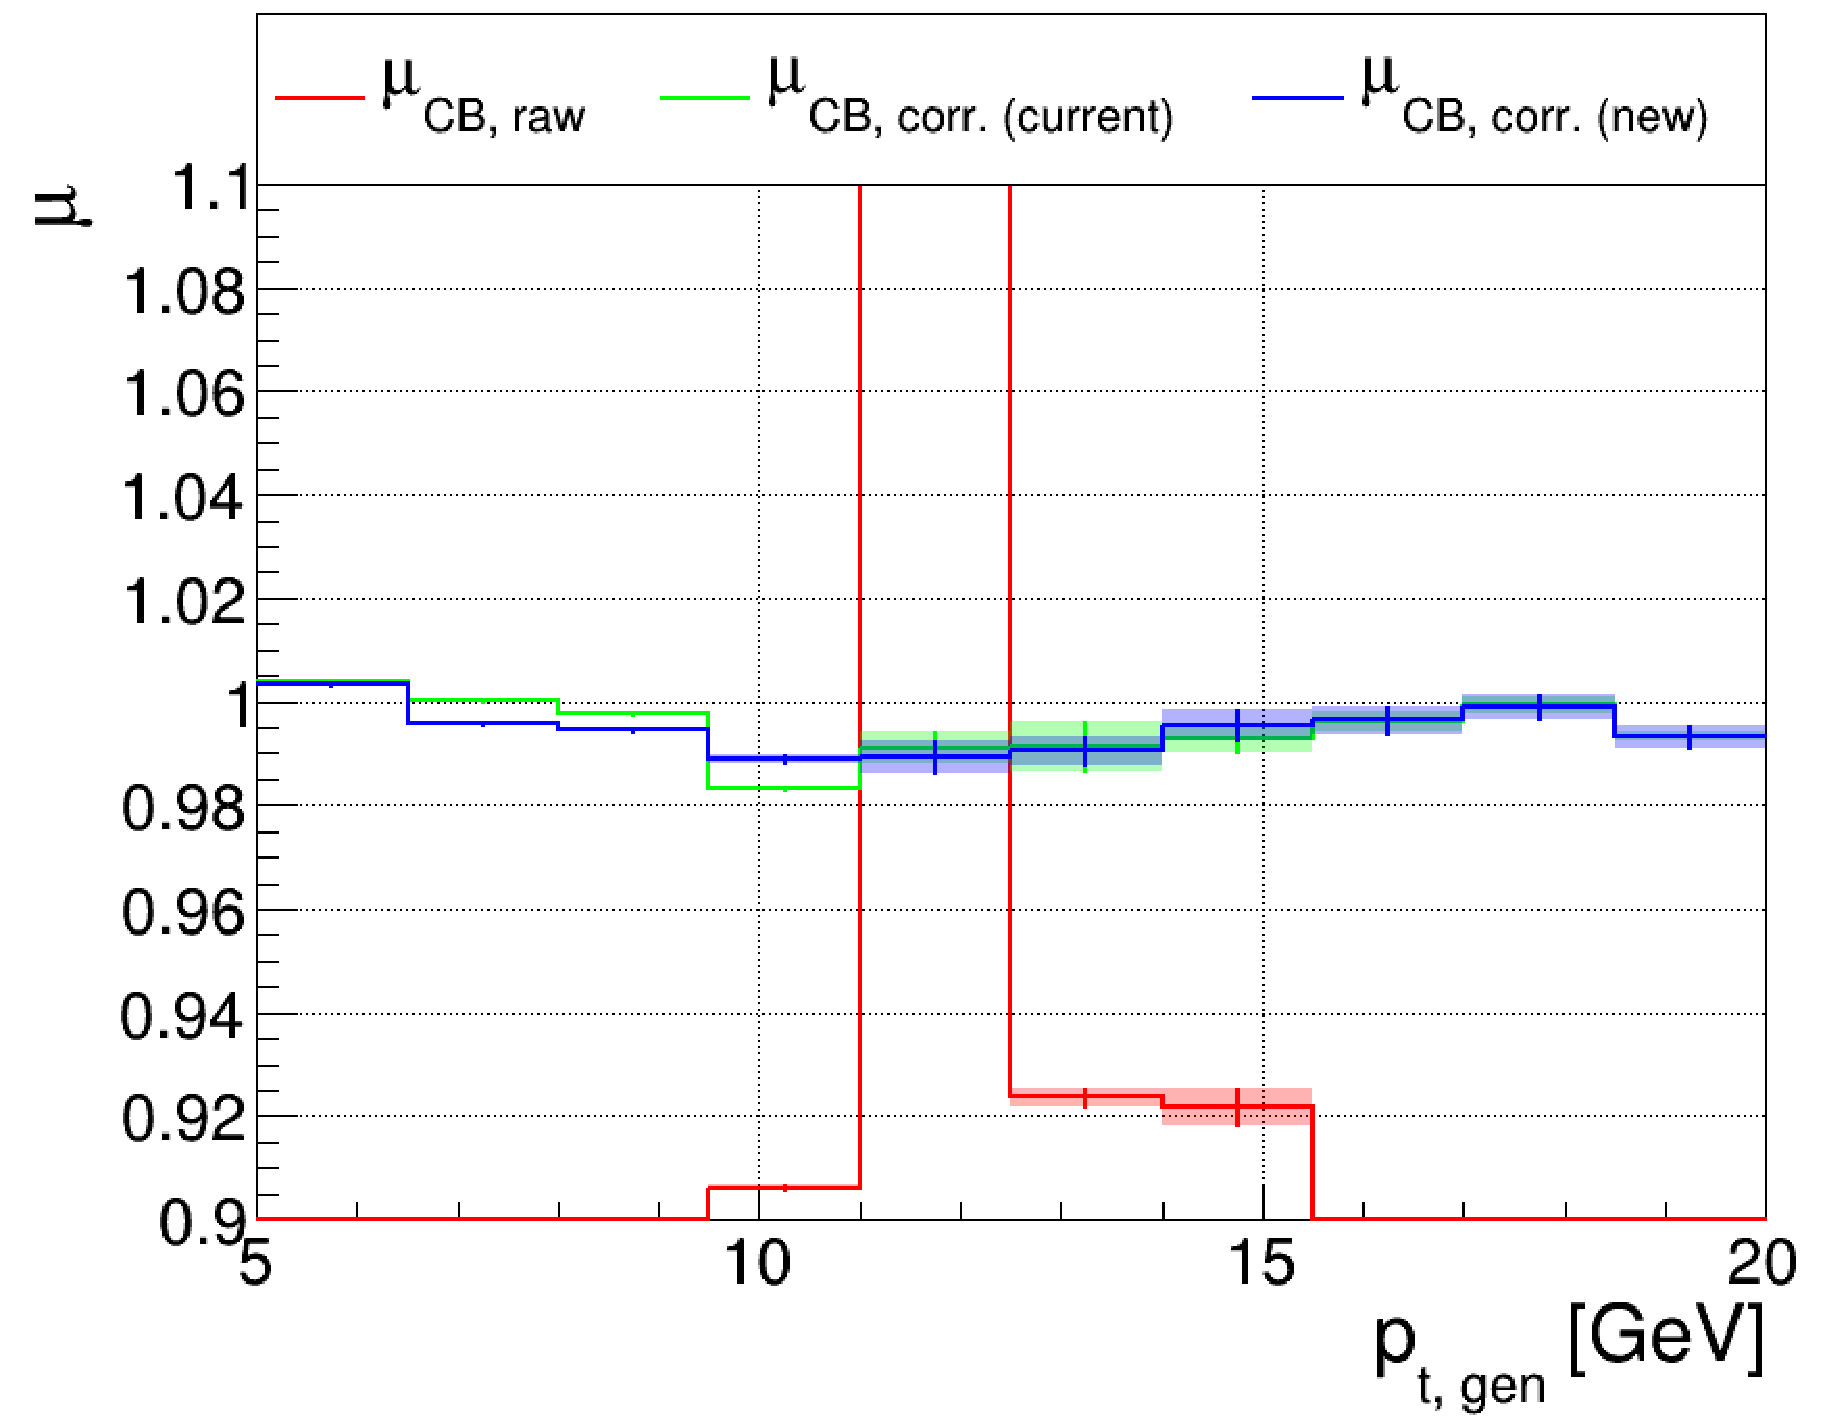
\includegraphics[width=0.495\textwidth]{./plots_pdf/ECAL_plots/plotsNoPU/EE/pdf/FULL/GENPT/EEFULL_GENPT_0005_0020_MuOverBins.pdf}
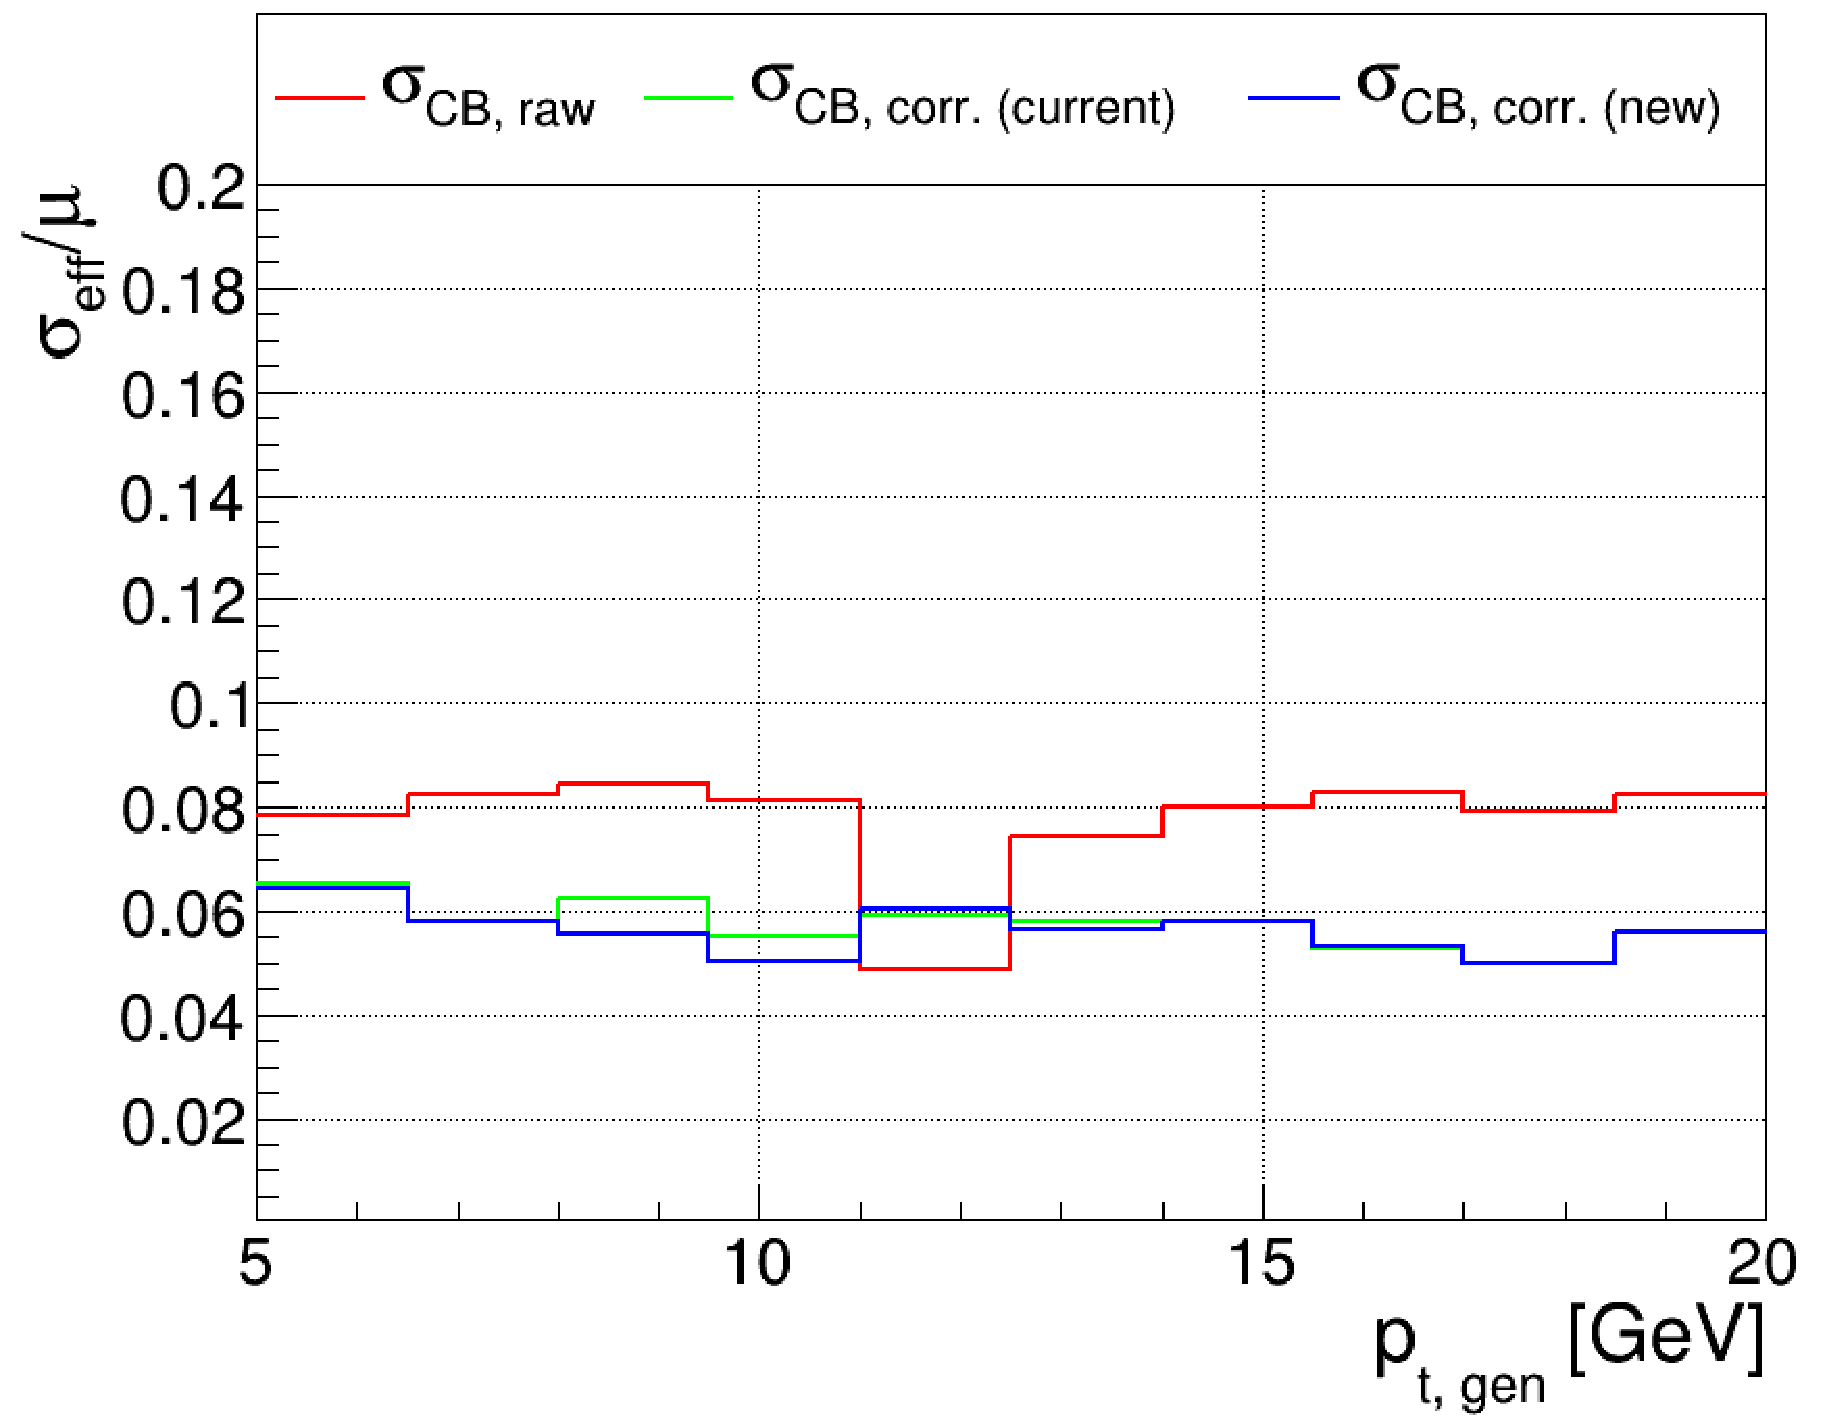
\includegraphics[width=0.495\textwidth]{./plots_pdf/ECAL_plots/plotsNoPU/EE/pdf/FULL/GENPT/EEFULL_GENPT_0005_0020_EffSigmaOverBins.pdf}

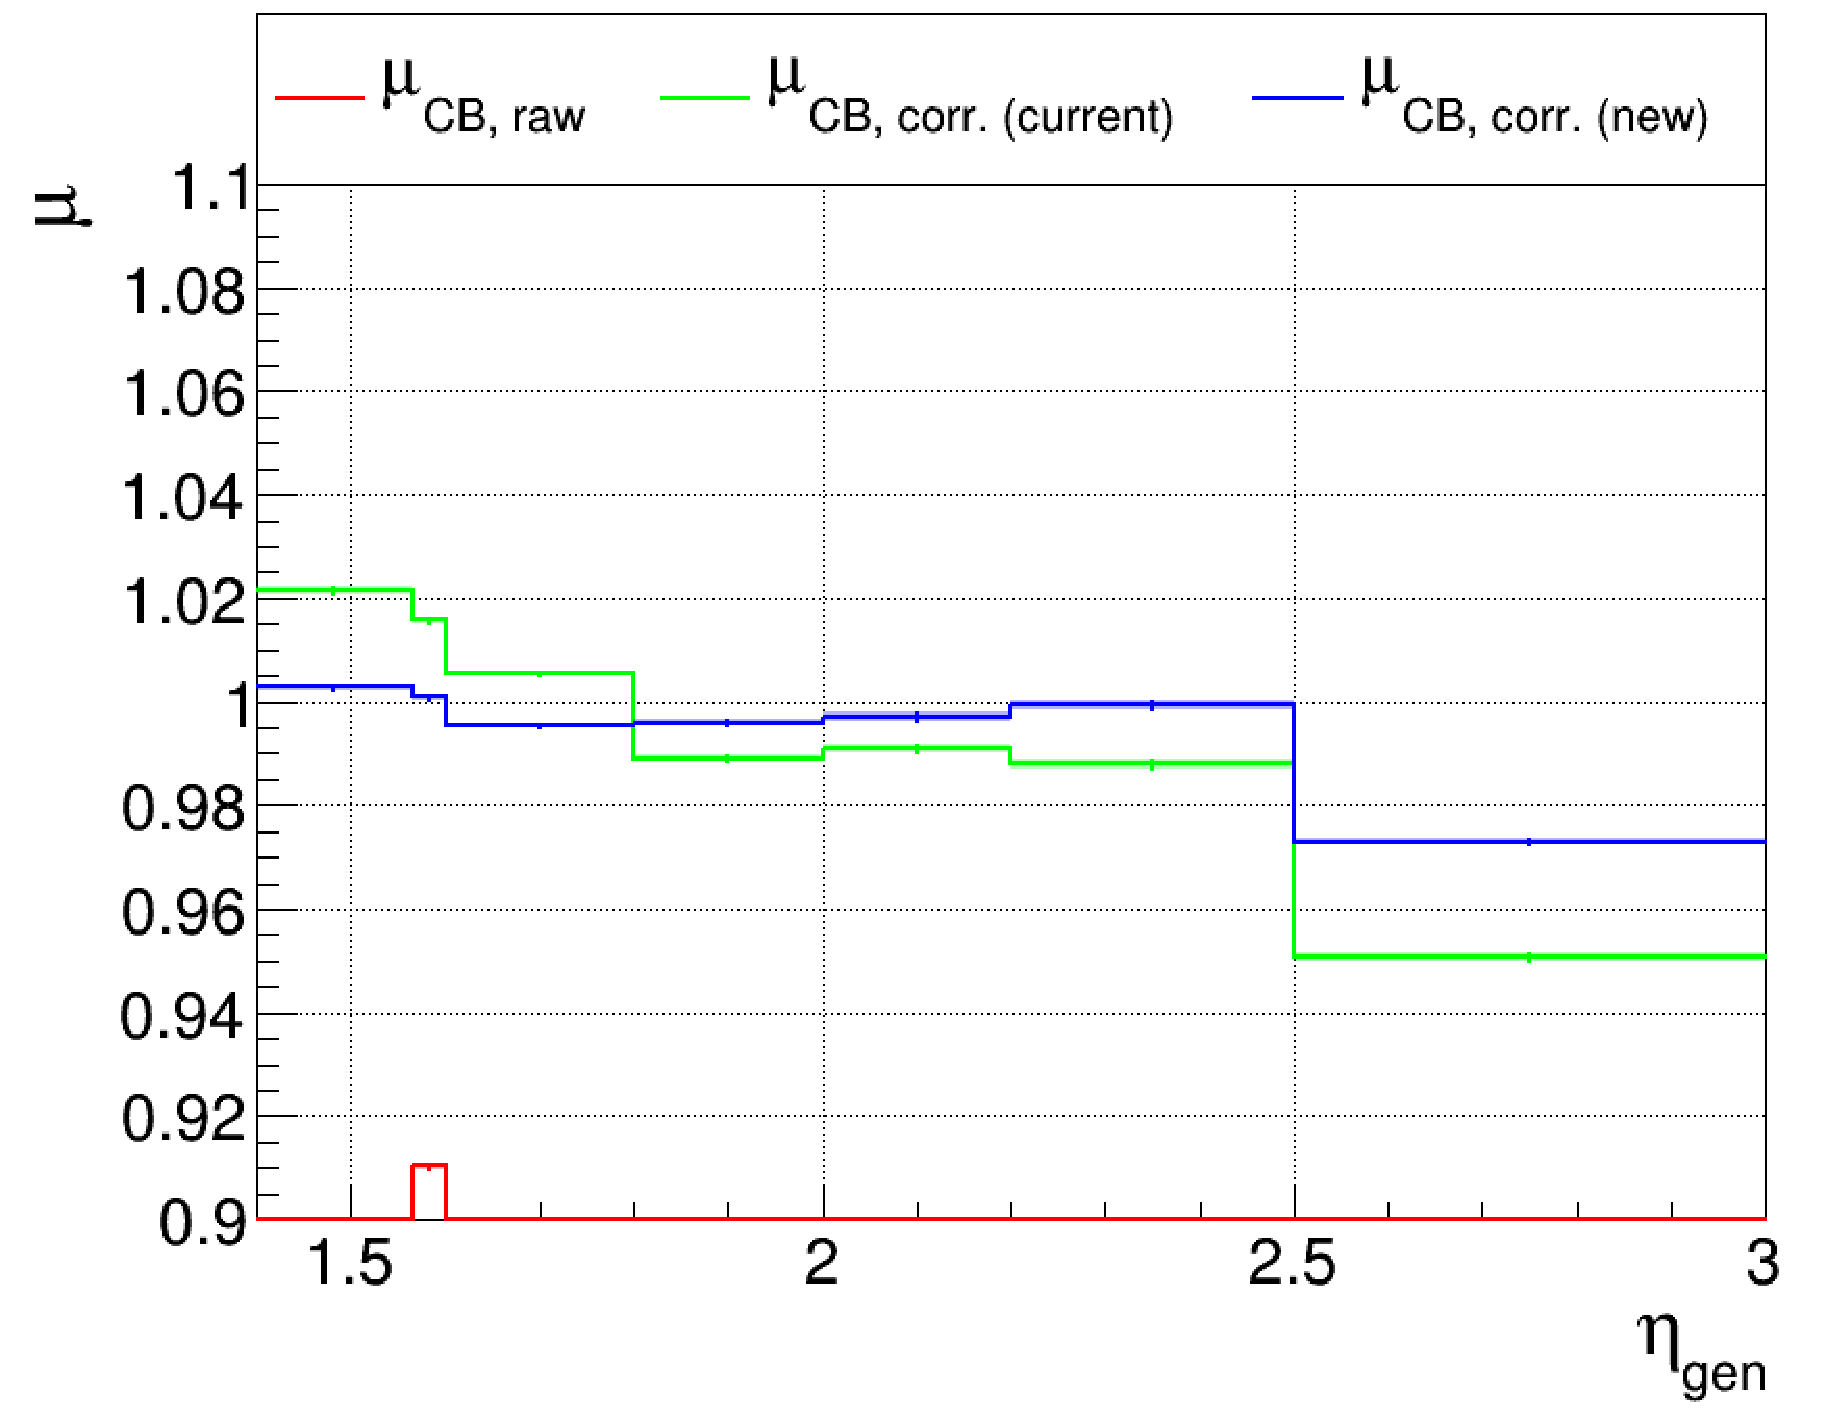
\includegraphics[width=0.495\textwidth]{./plots_pdf/ECAL_plots/plotsNoPU/EE/pdf/FULL/GENETA/EEFULL_GENETA_0005_0020_MuOverBins.pdf}
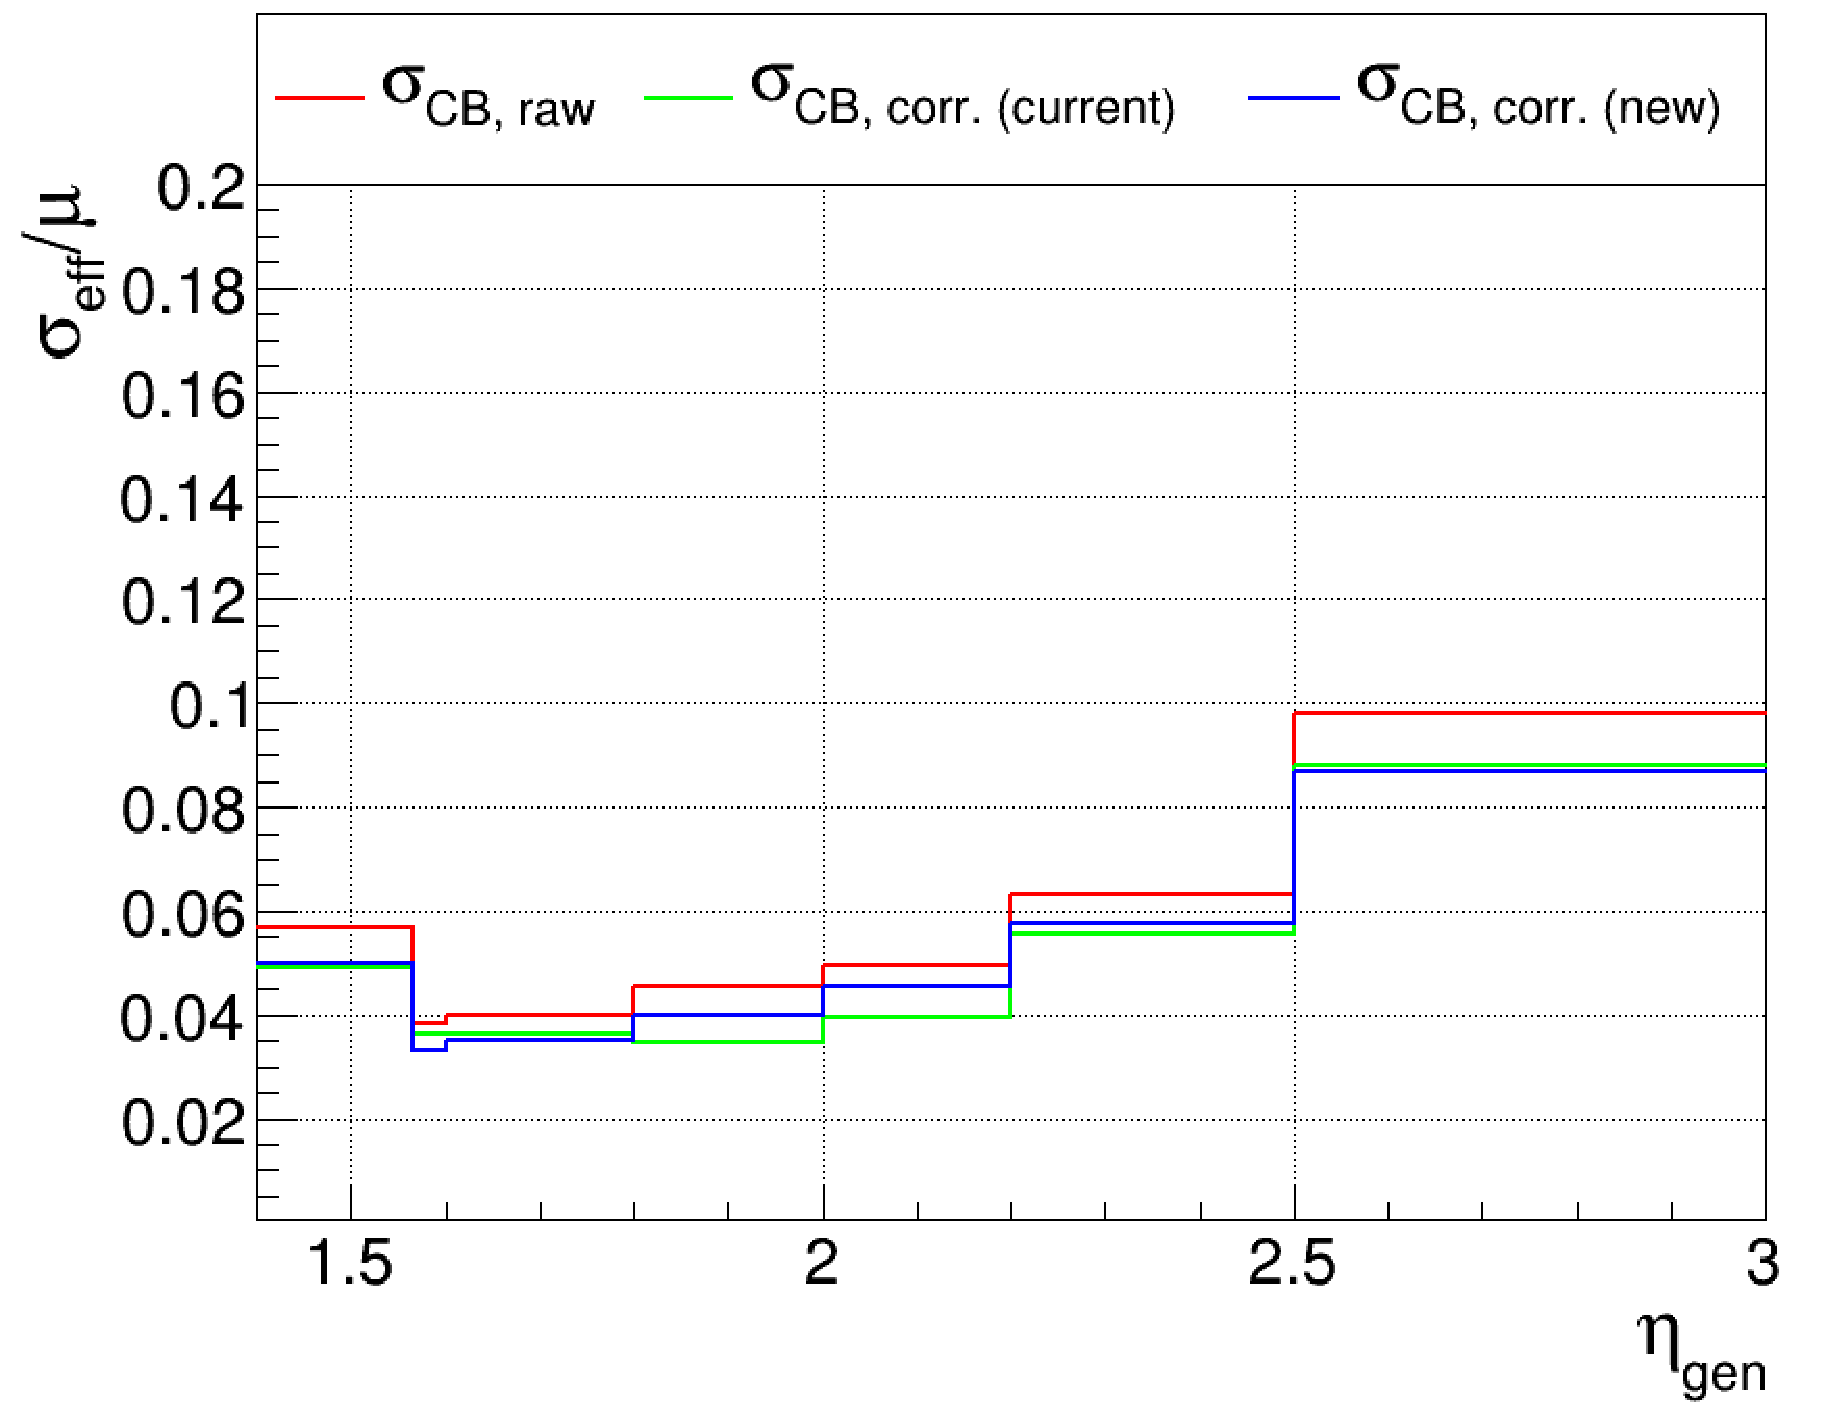
\includegraphics[width=0.495\textwidth]{./plots_pdf/ECAL_plots/plotsNoPU/EE/pdf/FULL/GENETA/EEFULL_GENETA_0005_0020_EffSigmaOverBins.pdf}
\caption{EE - Full Readout \pt 5-20}
%\end{figure}


%\begin{figure}
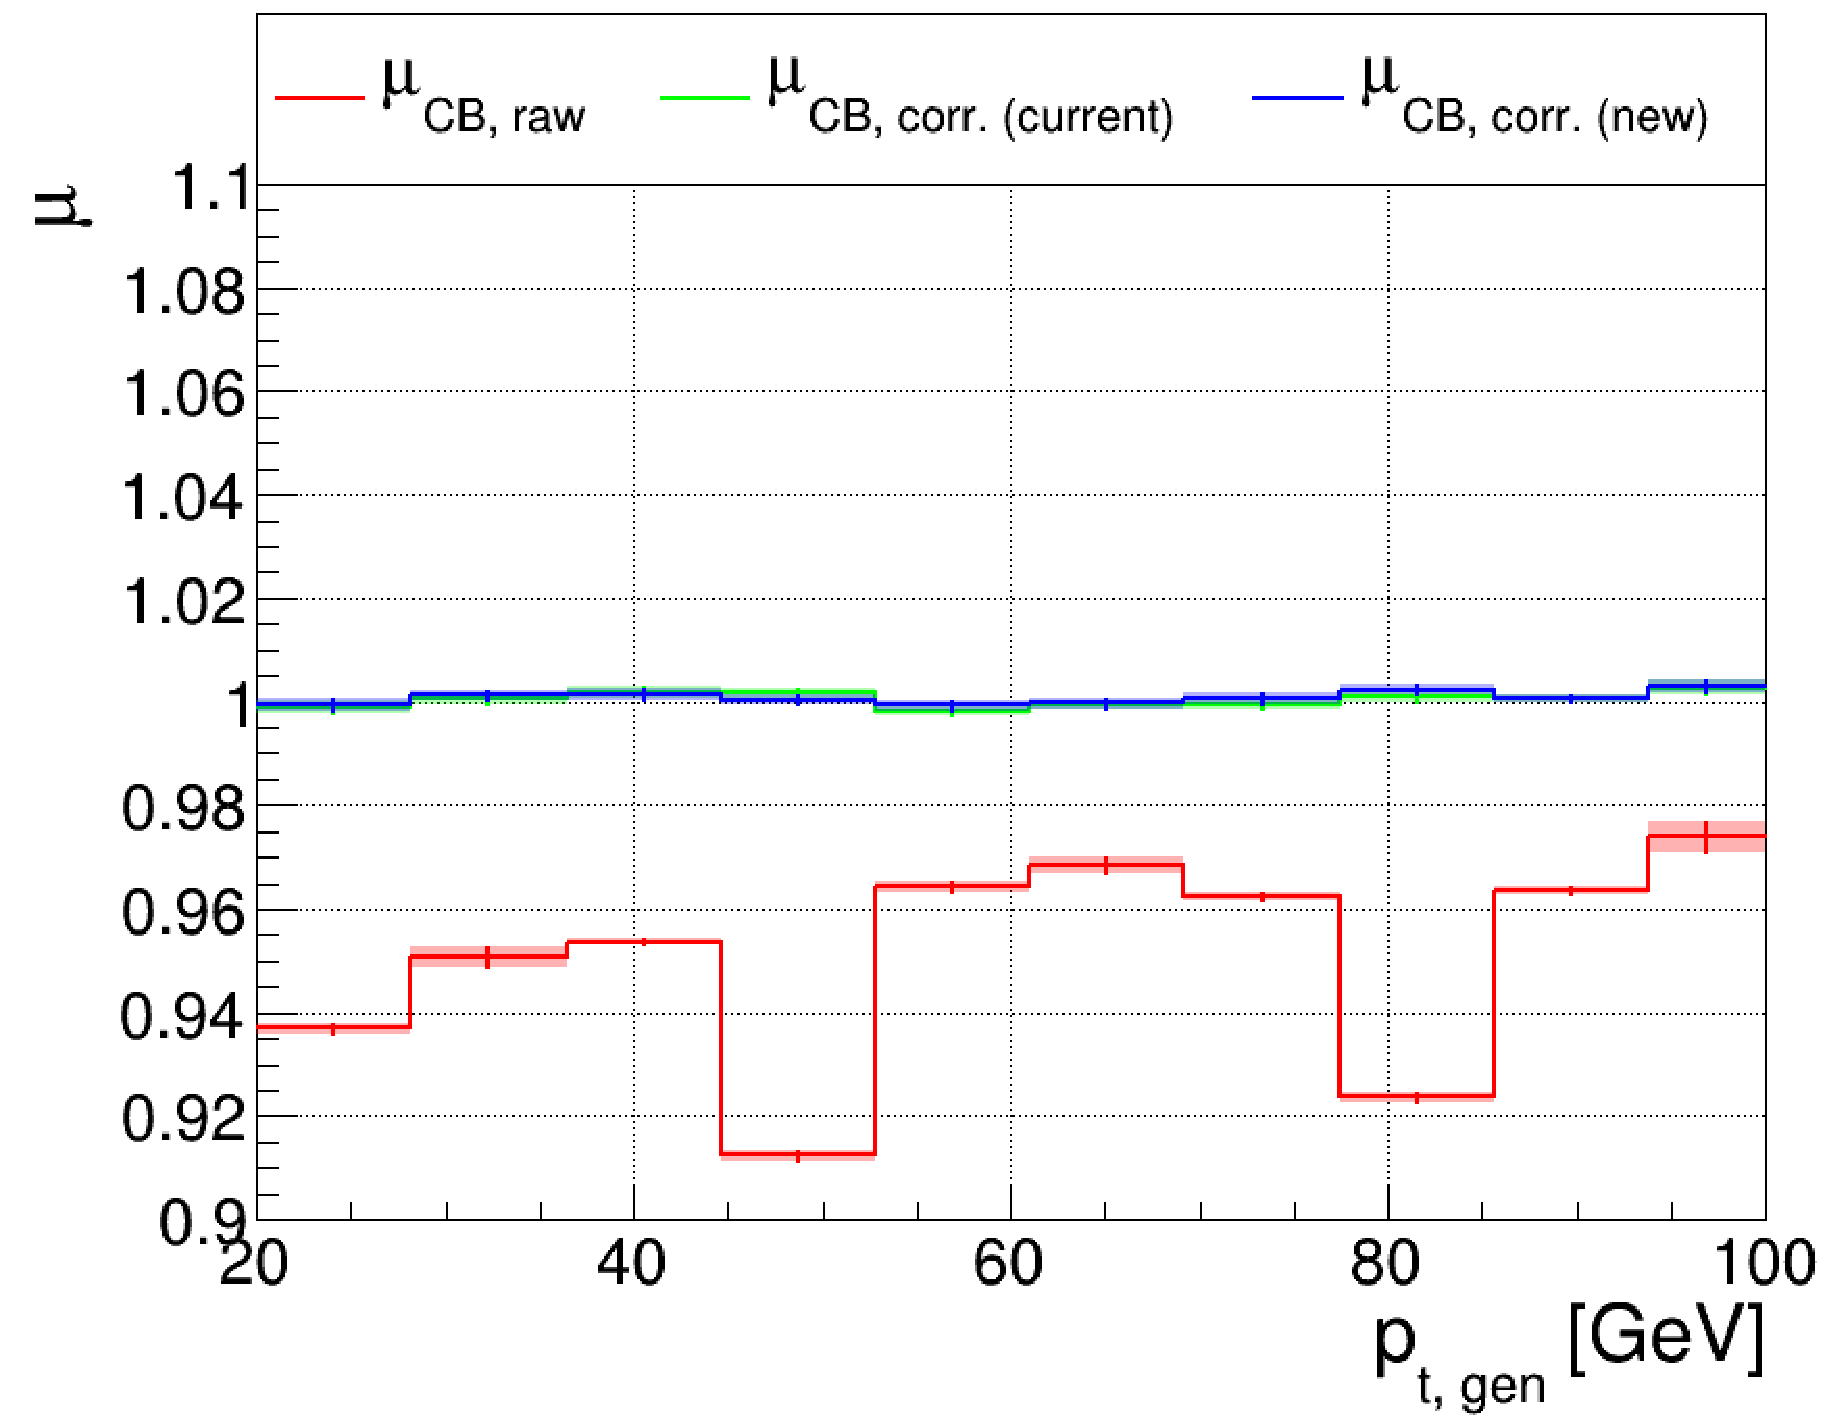
\includegraphics[width=0.495\textwidth]{./plots_pdf/ECAL_plots/plotsNoPU/EE/pdf/FULL/GENPT/EEFULL_GENPT_0020_0100_MuOverBins.pdf}
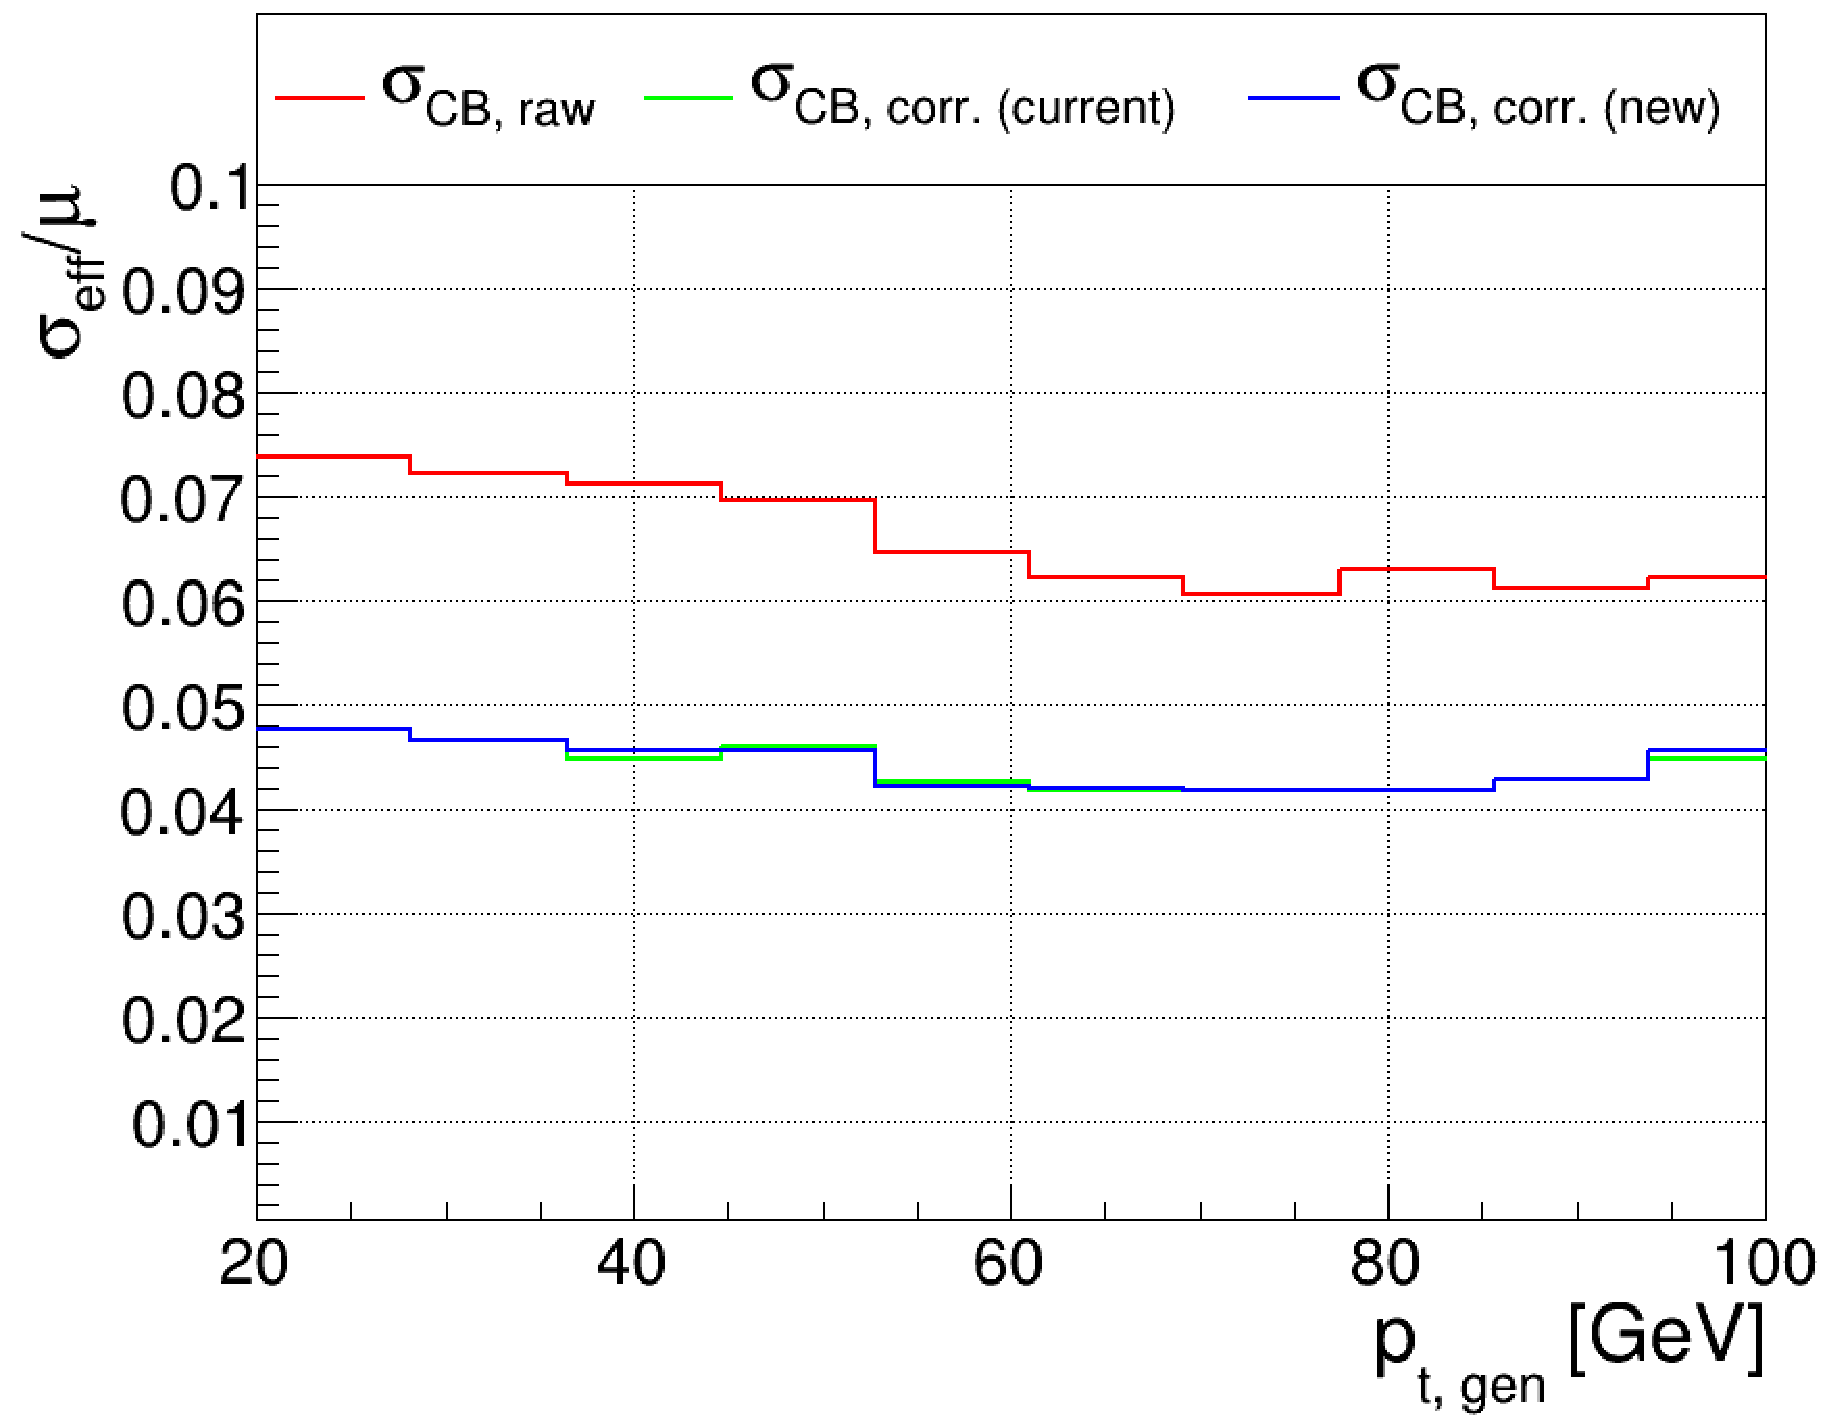
\includegraphics[width=0.495\textwidth]{./plots_pdf/ECAL_plots/plotsNoPU/EE/pdf/FULL/GENPT/EEFULL_GENPT_0020_0100_EffSigmaOverBins.pdf}

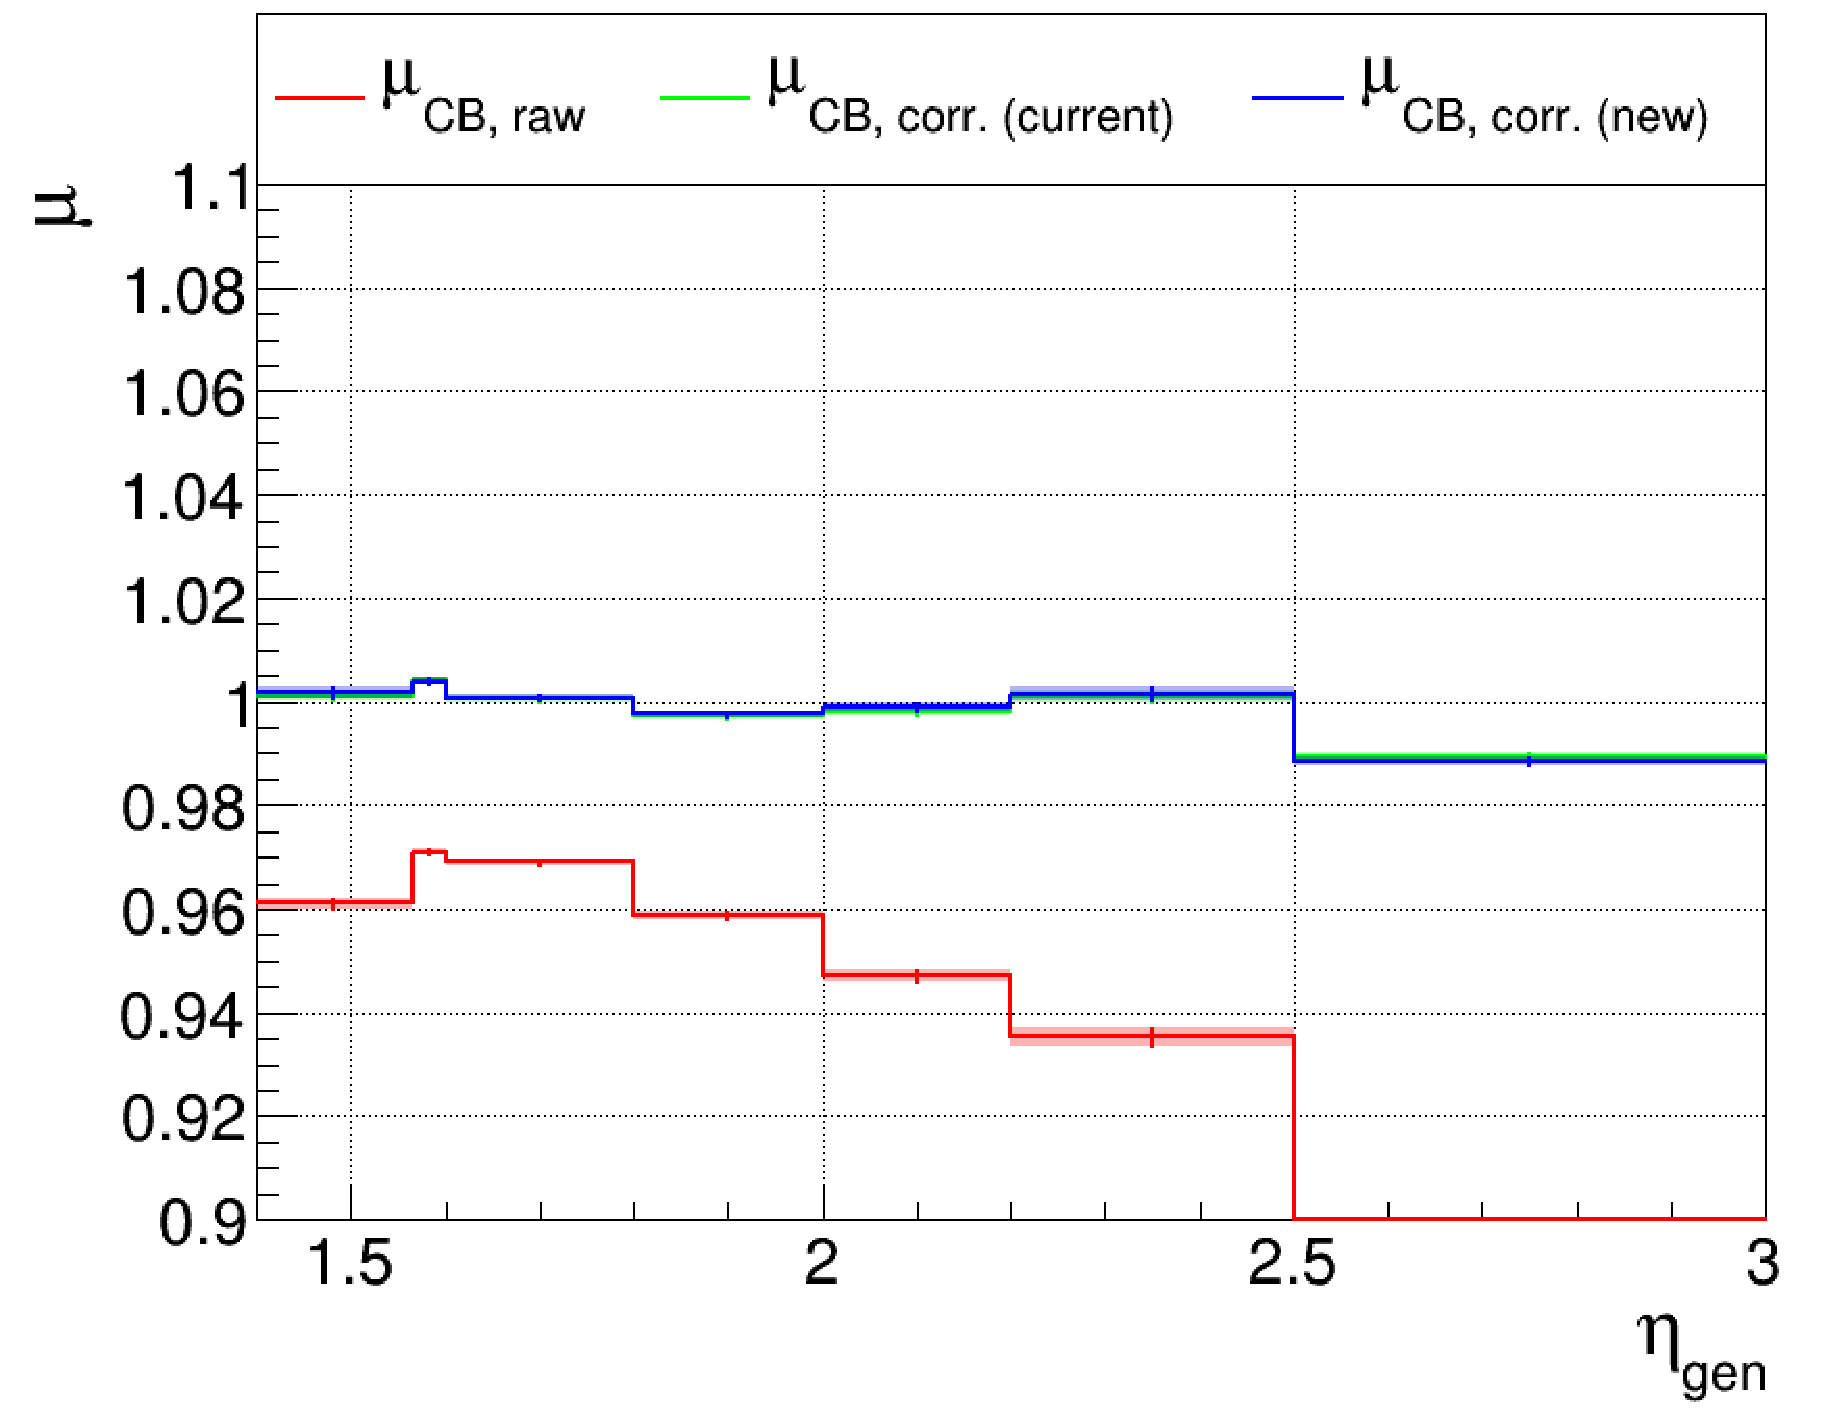
\includegraphics[width=0.495\textwidth]{./plots_pdf/ECAL_plots/plotsNoPU/EE/pdf/FULL/GENETA/EEFULL_GENETA_0020_0100_MuOverBins.pdf}
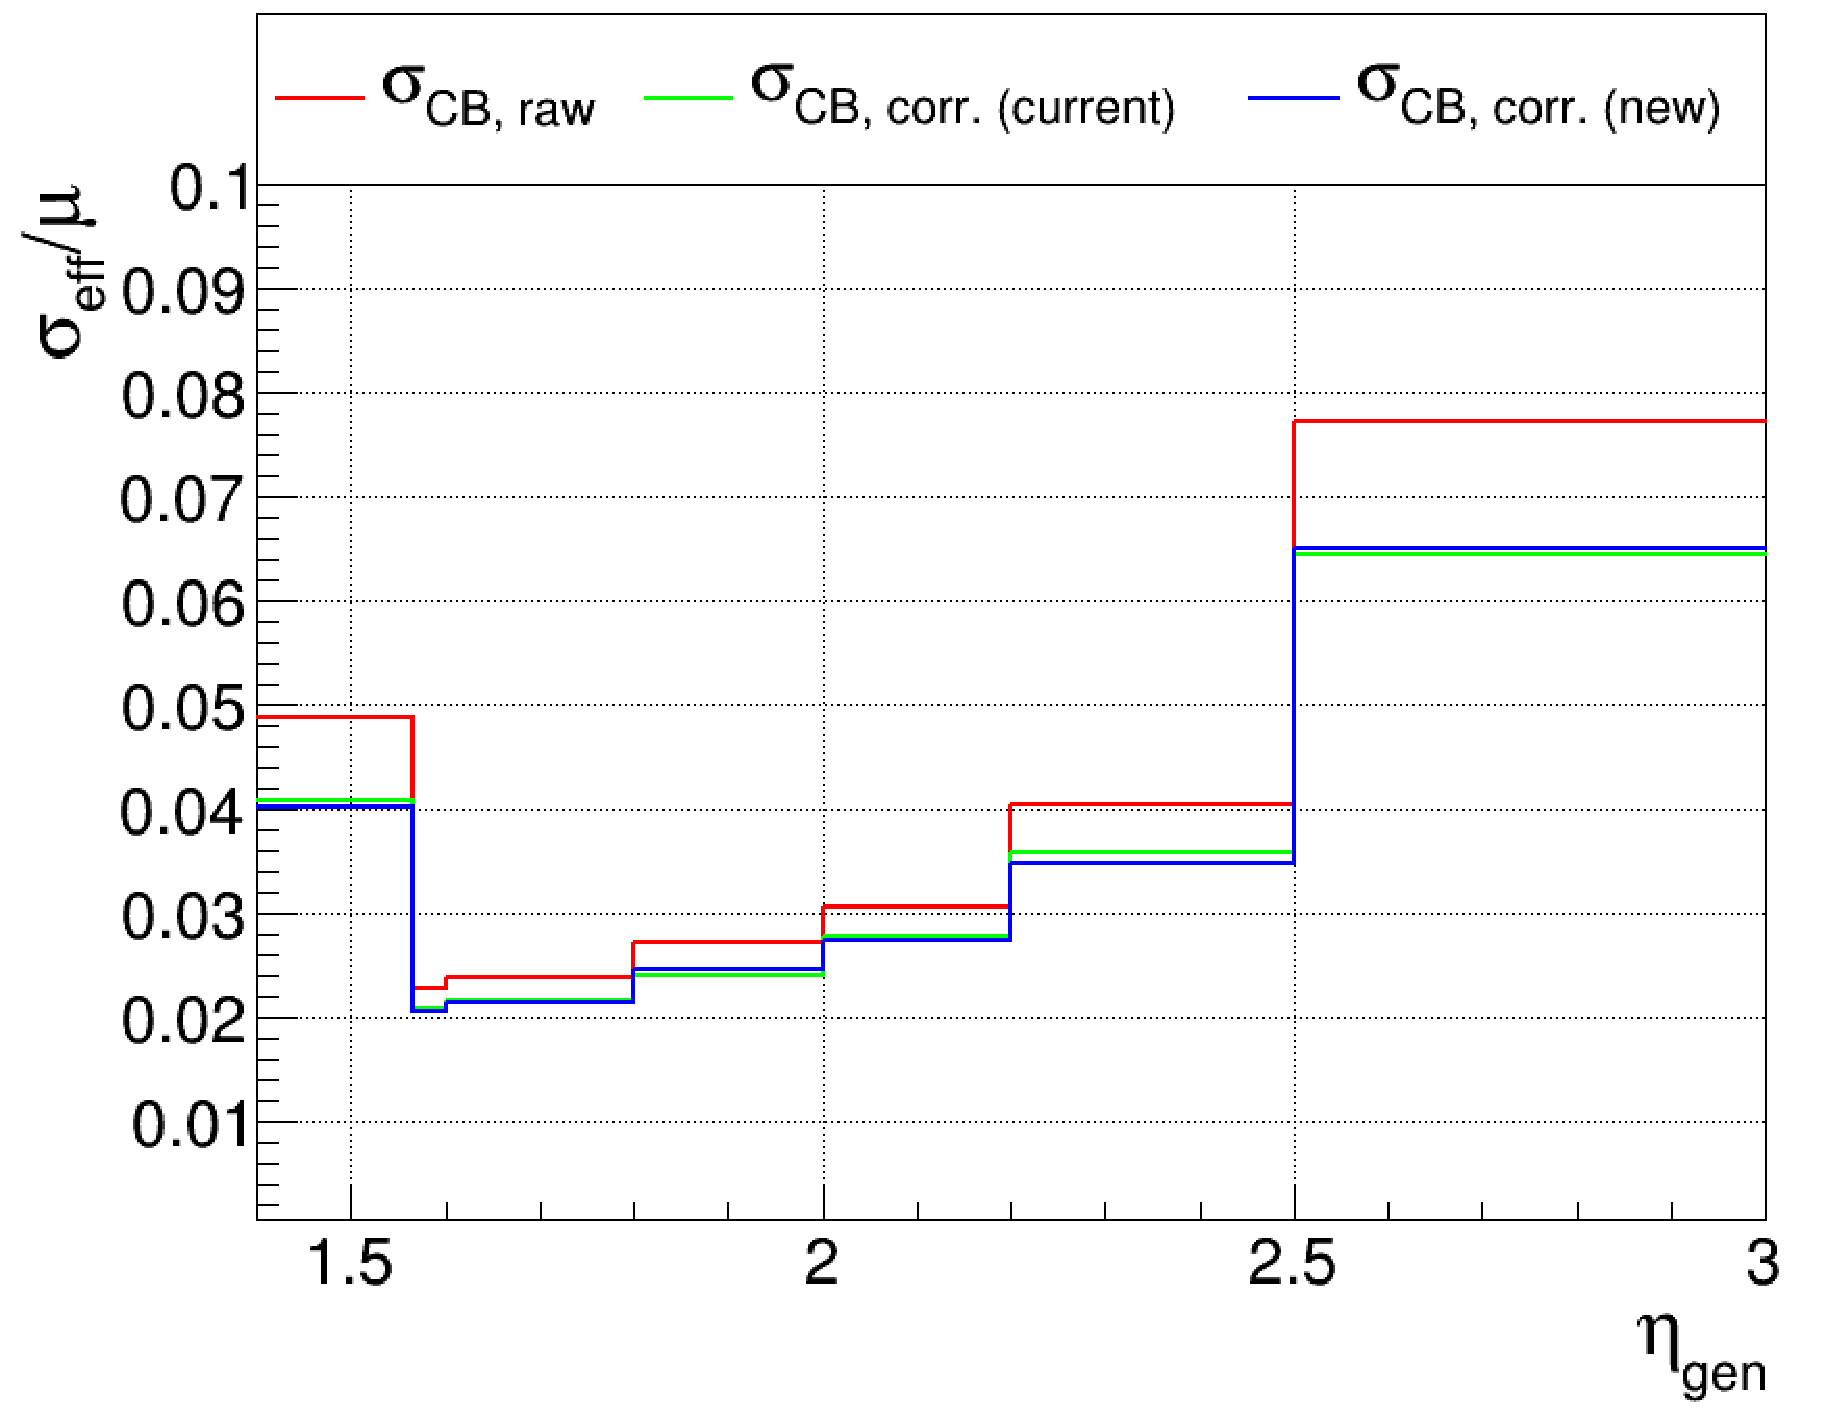
\includegraphics[width=0.495\textwidth]{./plots_pdf/ECAL_plots/plotsNoPU/EE/pdf/FULL/GENETA/EEFULL_GENETA_0020_0100_EffSigmaOverBins.pdf}
\caption{EE - Full Readout \pt 20-100}
\end{figure}


\begin{figure}
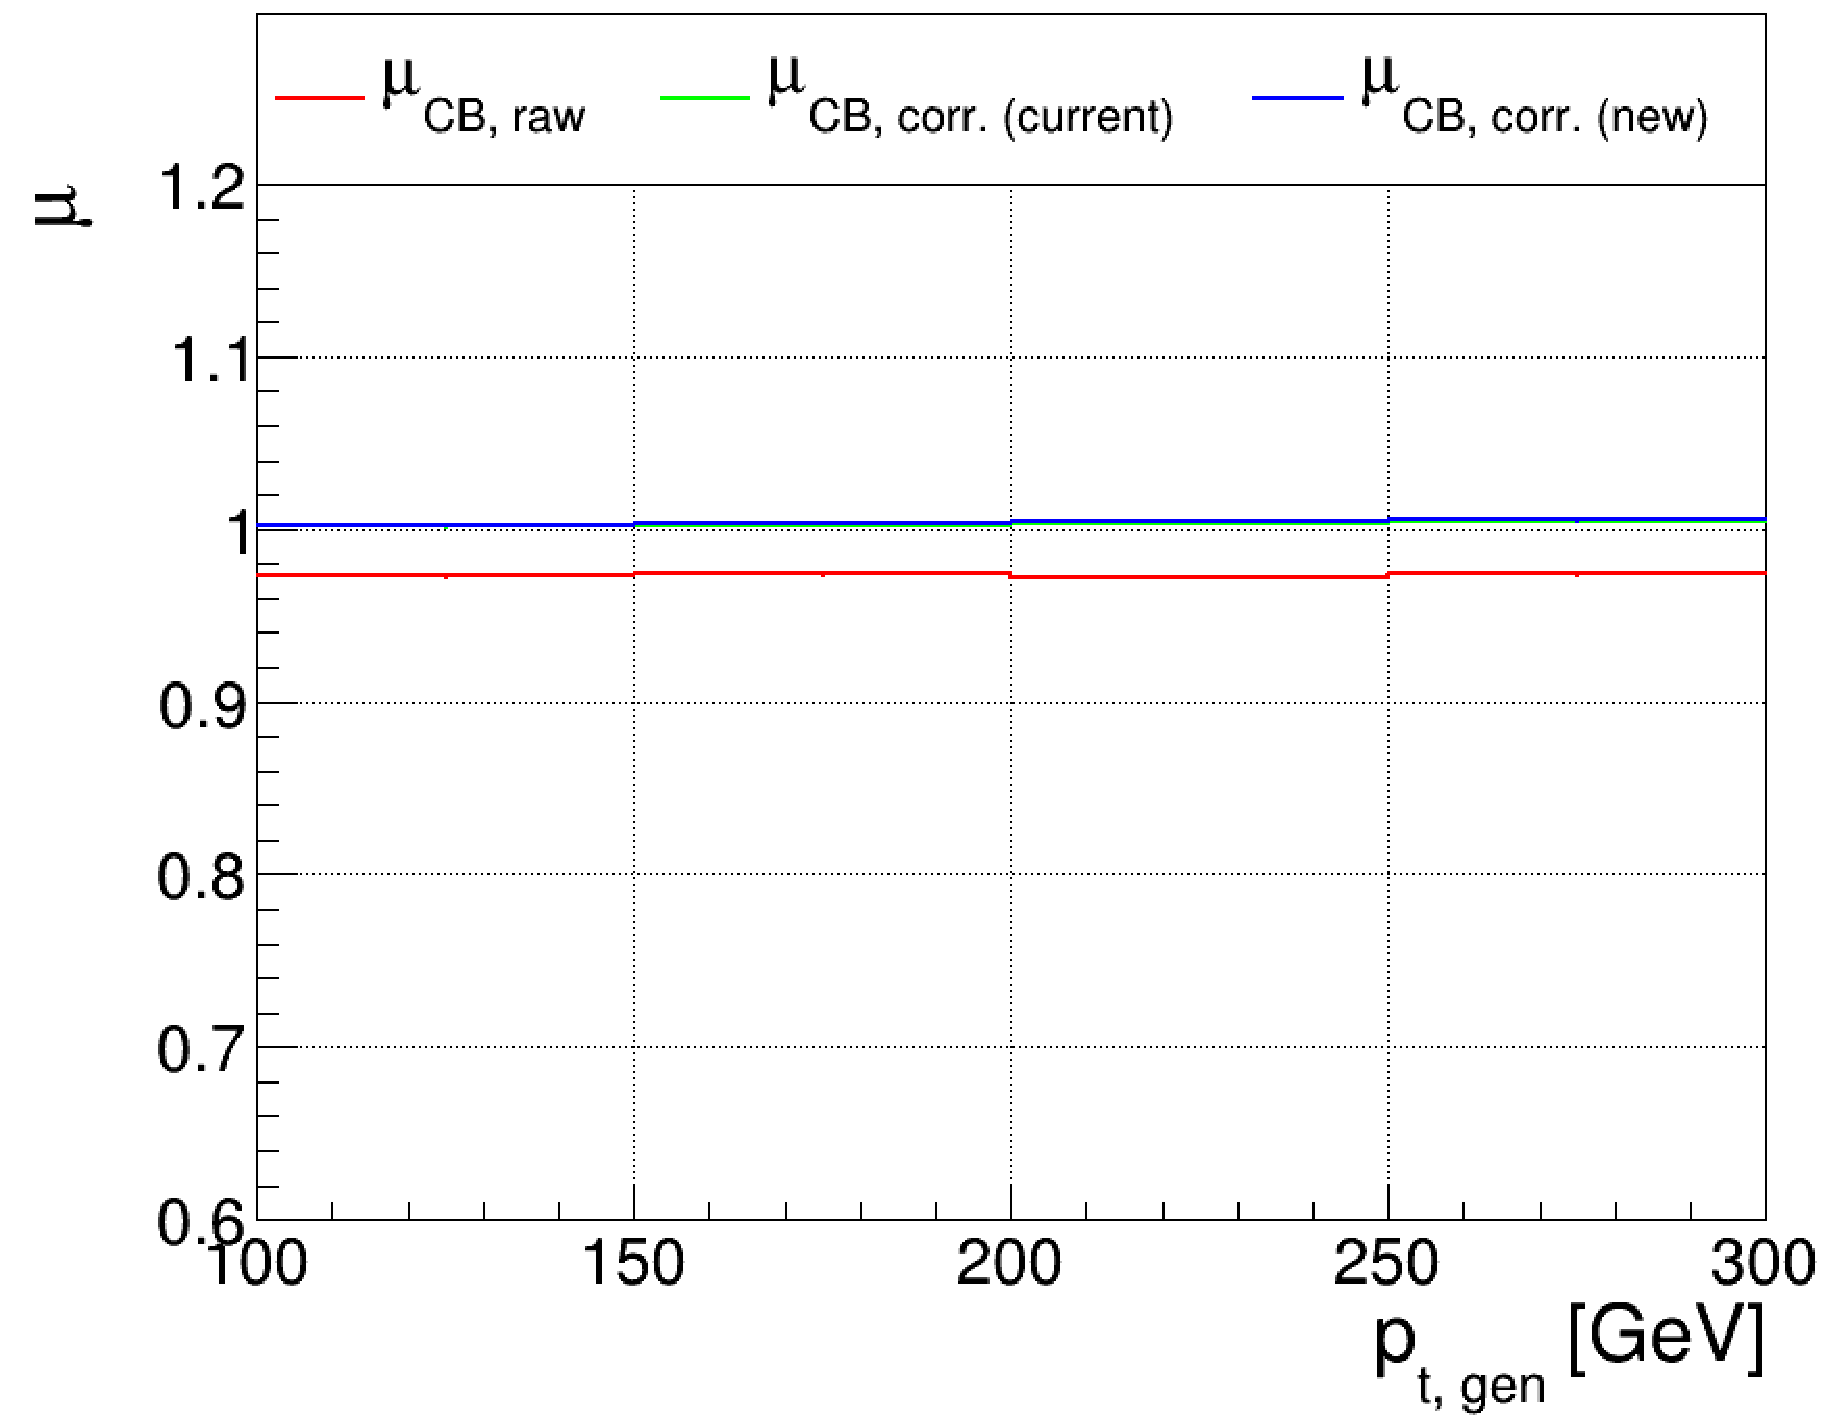
\includegraphics[width=0.495\textwidth]{./plots_pdf/ECAL_plots/plotsNoPU/EE/pdf/FULL/GENPT/EEFULL_GENPT_0100_0300_MuOverBins.pdf}
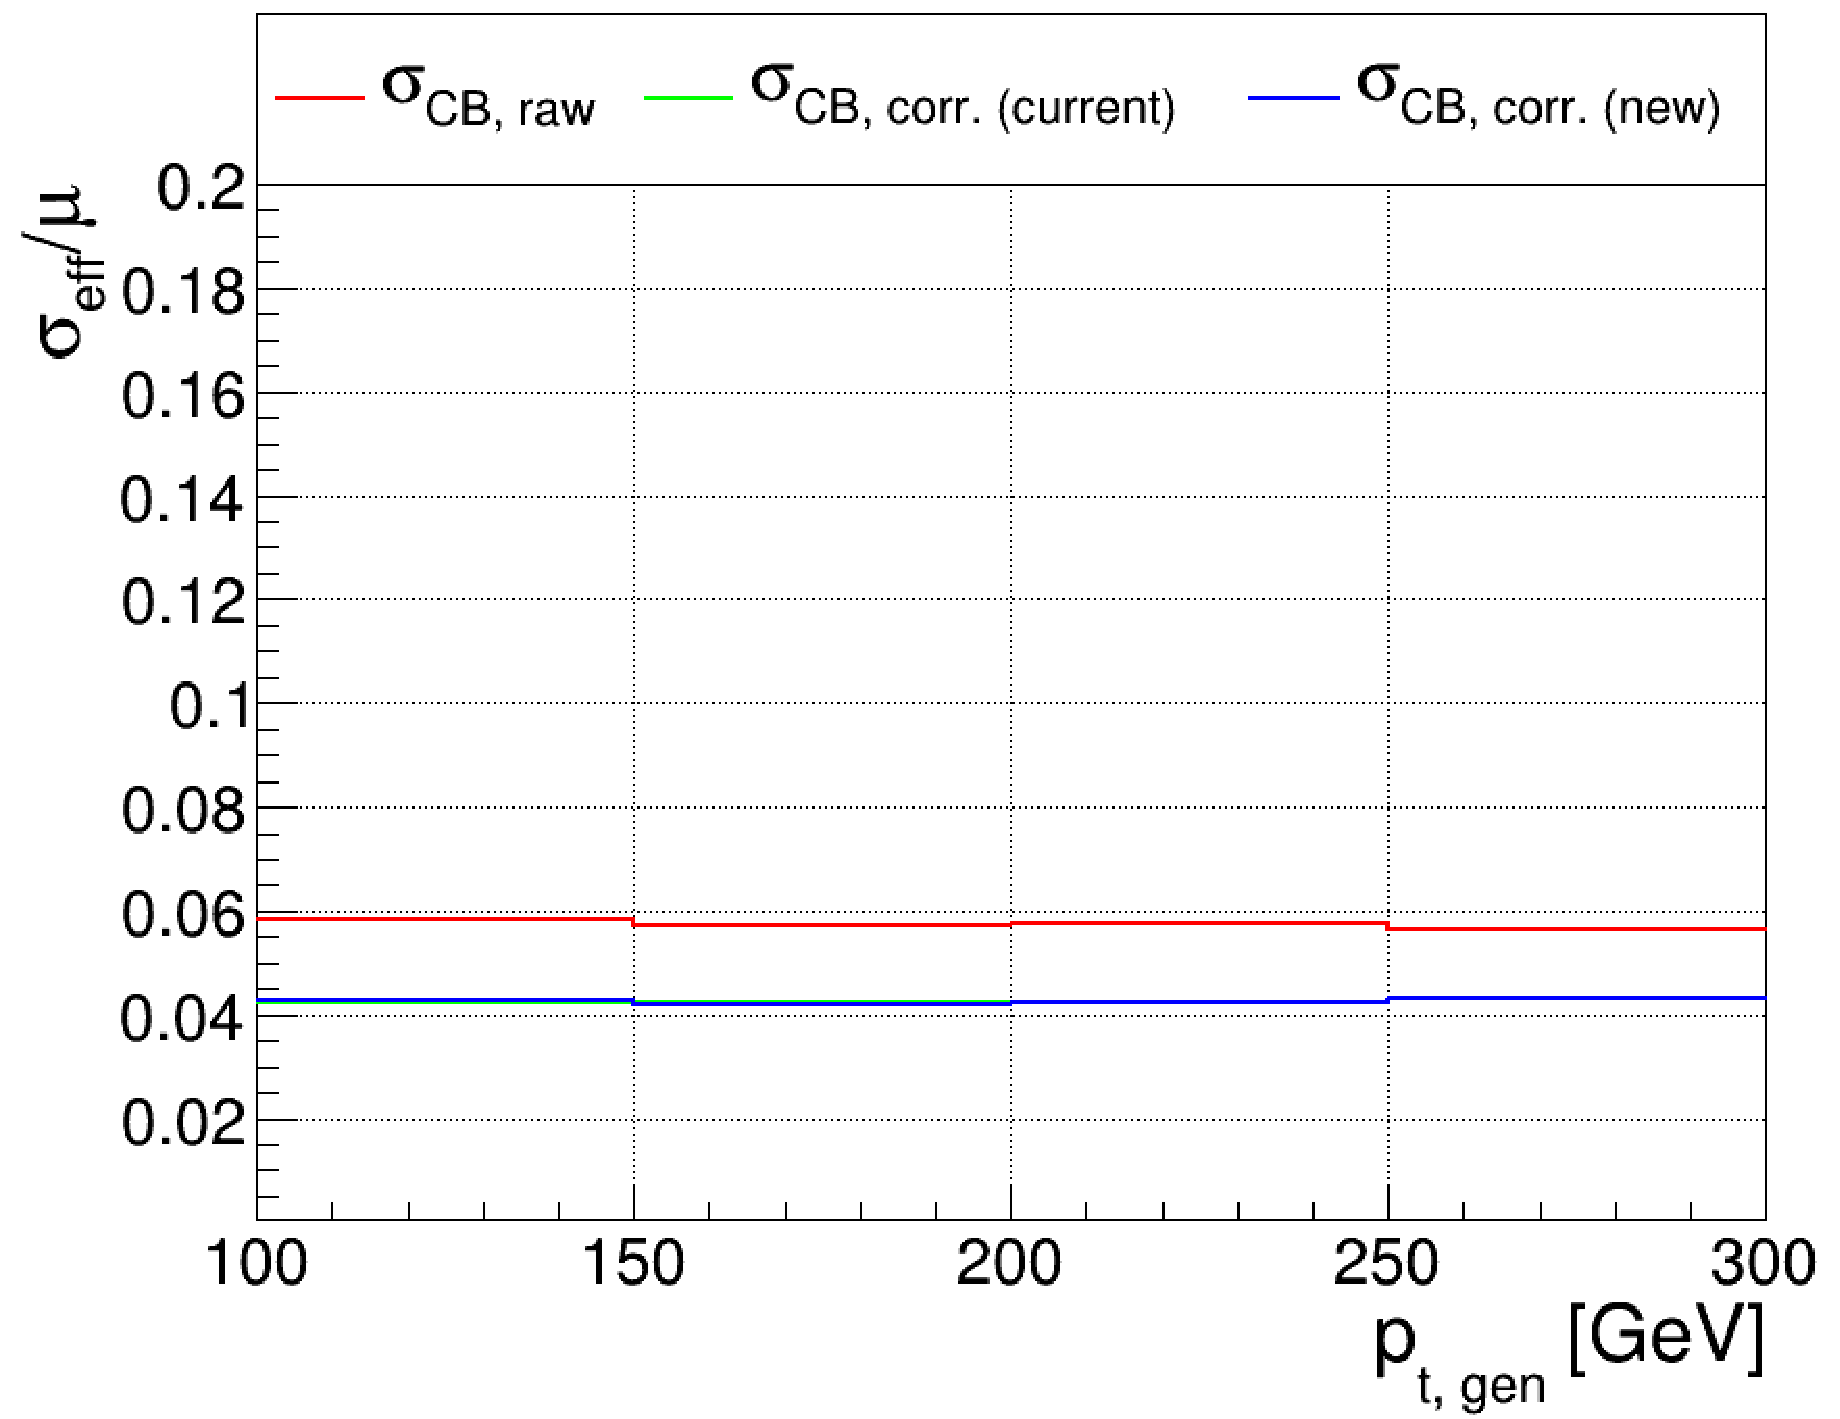
\includegraphics[width=0.495\textwidth]{./plots_pdf/ECAL_plots/plotsNoPU/EE/pdf/FULL/GENPT/EEFULL_GENPT_0100_0300_EffSigmaOverBins.pdf}
%\caption{EE - Full Readout pt 100-300}
%\end{figure}
%\begin{figure}
\includegraphics[width=0.495\textwidth]{./plots_pdf/ECAL_plots/plotsNoPU/EE/pdf/FULL/GENETA/EEFULL_GENETA_0100_0300_MuOverBins.pdf}
\includegraphics[width=0.495\textwidth]{.plots_pdf/ECAL_plots/plotsNoPU/EE/pdf/FULL/GENETA/EEFULL_GENETA_0100_0300_EffSigmaOverBins.pdf}
\caption{EE - Full Readout \pt 100-300}
\end{figure}





\begin{figure}
\includegraphics[width=0.495\textwidth]{./plots_pdf/ECAL_plots/plotsNoPU/EE/pdf/ZS/GENPT/EEZS_GENPT_0000_0006_MuOverBins.pdf}
\includegraphics[width=0.495\textwidth]{./plots_pdf/ECAL_plots/plotsNoPU/EE/pdf/ZS/GENPT/EEZS_GENPT_0000_0006_EffSigmaOverBins.pdf}

\includegraphics[width=0.495\textwidth]{./plots_pdf/ECAL_plots/plotsNoPU/EE/pdf/ZS/GENETA/EEZS_GENETA_0000_0006_MuOverBins.pdf}
\includegraphics[width=0.495\textwidth]{./plots_pdf/ECAL_plots/plotsNoPU/EE/pdf/ZS/GENETA/EEZS_GENETA_0000_0006_EffSigmaOverBins.pdf}
\caption[$\mu$ ($\sigma_\mathrm{eff}$) vs \pt of PF ECAL cluster - EE ZS readout NoPU scenario]{Mean response (resolution) defined by Raw PF ECAL clusters (red), the calibration derived earlier in Ru\
n3 based on 126X (green), and the new correction from 2024 simulation sample based on 133X (blue).\pt 0--6\GeV in EE region ZS Readout NOPU scenario.}
\end{figure}

%% %\begin{figure}
%% \includegraphics[width=0.495\textwidth]{./plots_pdf/ECAL_plots/plotsNoPU/EE/pdf/ZS/GENPT/EEZS_GENPT_0006_0025_MuOverBins.pdf}
%% \includegraphics[width=0.495\textwidth]{./plots_pdf/ECAL_plots/plotsNoPU/EE/pdf/ZS/GENPT/EEZS_GENPT_0006_0025_EffSigmaOverBins.pdf}
%% %\caption{EE - ZS Readout pt 6-25}
%% %\end{figure}
%% %\begin{figure}
%% \includegraphics[width=0.495\textwidth]{./plots_pdf/ECAL_plots/plotsNoPU/EE/pdf/ZS/GENETA/EEZS_GENETA_0006_0025_MuOverBins.pdf}
%% %\includegraphics[width=0.495\textwidth]{./ECAL_plots/plotsNoPU/EE/pdf/ZS/GENETA/EEZS_GENETA_0006_0025_EffSigmaOverBins.pdf}
%% \caption{EE - ZS Readout \pt 6-25}
%% \end{figure}




\begin{figure}
\includegraphics[width=0.495\textwidth]{./plots_pdf/ECAL_plots/plotsPU/EE/FULL/pdf/GENPT/EEFULL_GENPT_0005_0020_MuOverBins.pdf}
\includegraphics[width=0.495\textwidth]{./plots_pdf/ECAL_plots/plotsPU/EE/FULL/pdf/GENPT/EEFULL_GENPT_0005_0020_EffSigmaOverBins.pdf}
\includegraphics[width=0.495\textwidth]{./plots_pdf/ECAL_plots/plotsPU/EE/FULL/pdf/GENPT/EEFULL_GENPT_0020_0100_MuOverBins.pdf}
\includegraphics[width=0.495\textwidth]{./plots_pdf/ECAL_plots/plotsPU/EE/FULL/pdf/GENPT/EEFULL_GENPT_0020_0100_EffSigmaOverBins.pdf}
\includegraphics[width=0.495\textwidth]{./plots_pdf/ECAL_plots/plotsPU/EE/FULL/pdf/GENPT/EEFULL_GENPT_0100_0300_MuOverBins.pdf}
\includegraphics[width=0.495\textwidth]{./plots_pdf/ECAL_plots/plotsPU/EE/FULL/pdf/GENPT/EEFULL_GENPT_0100_0300_EffSigmaOverBins.pdf}

\caption [$\mu$ ($\sigma_\mathrm{eff}$) vs \pt of PF ECAL cluster - EE full readout PU scenario]{Mean response (resolution) defined by Raw PF ECAL clusters (red), the calibration derived earlier in Ru\
n3 based on 126X (green), and the new correction from 2024 simulation sample based on 133X (blue). (top) low \pt, (middle) mid \pt, (bottom) high \pt in EE region full readout PU scenario.}
\label{fig:PU_EEFULL_pt}
\end{figure}


\begin{figure}
\includegraphics[width=0.495\textwidth]{./plots_pdf/ECAL_plots/plotsPU/EE/FULL/pdf/GENETA/EEFULL_GENETA_0005_0020_MuOverBins.pdf}
\includegraphics[width=0.495\textwidth]{./plots_pdf/ECAL_plots/plotsPU/EE/FULL/pdf/GENETA/EEFULL_GENETA_0005_0020_EffSigmaOverBins.pdf}
\includegraphics[width=0.495\textwidth]{./plots_pdf/ECAL_plots/plotsPU/EE/FULL/pdf/GENETA/EEFULL_GENETA_0020_0100_MuOverBins.pdf}
\includegraphics[width=0.495\textwidth]{./plots_pdf/ECAL_plots/plotsPU/EE/FULL/pdf/GENETA/EEFULL_GENETA_0020_0100_EffSigmaOverBins.pdf}
\includegraphics[width=0.495\textwidth]{./plots_pdf/ECAL_plots/plotsPU/EE/FULL/pdf/GENETA/EEFULL_GENETA_0100_0300_MuOverBins.pdf}
\includegraphics[width=0.495\textwidth]{./plots_pdf/ECAL_plots/plotsPU/EE/FULL/pdf/GENETA/EEFULL_GENETA_0100_0300_EffSigmaOverBins.pdf}


\caption [$\mu$ ($\sigma_\mathrm{eff}$) vs $\eta$ of PF ECAL cluster - EE Full readout PU scenario]{Mean response (resolution) defined by Raw PF ECAL clusters (red), the calibration derived earlier in\
 Run3 based on 126X (green), and the new correction from 2024 simulation sample based on 133X (blue). (top) low $\eta$, (middle) mid $\eta$, (bottom) high $\eta$ in EE region Full readout PU scenario.}
\label{fig:PU_EEFULL_eta}
\end{figure}

\begin{figure}
\includegraphics[width=0.495\textwidth]{./plots_pdf/ECAL_plots/plotsPU/EE/ZS/pdf/GENPT/EEZS_GENPT_0000_0006_MuOverBins.pdf}
\includegraphics[width=0.495\textwidth]{./plots_pdf/ECAL_plots/plotsPU/EE/ZS/pdf/GENPT/EEZS_GENPT_0000_0006_EffSigmaOverBins.pdf}

\includegraphics[width=0.495\textwidth]{./plots_pdf/ECAL_plots/plotsPU/EE/ZS/pdf/GENETA/EEZS_GENETA_0000_0006_MuOverBins.pdf}
\includegraphics[width=0.495\textwidth]{./plots_pdf/ECAL_plots/plotsPU/EE/ZS/pdf/GENETA/EEZS_GENETA_0000_0006_EffSigmaOverBins.pdf}

\caption[$\mu$ ($\sigma_\mathrm{eff}$) vs. \pt of PF ECAL cluster - EE ZS readout PU scenario]{Mean response (resolution) defined by raw PF ECAL clusters (red), the calibration derived earlier in Run~3 based on 126X (green), and the new correction from the 2024 simulation sample based on 133X (blue).\pt 0--6\GeV in EE region ZS readout PU scenario.}
\label{fig:PU_EEZS}
\end{figure}

%% %\begin{figure}
%% \includegraphics[width=0.495\textwidth]{./plots_pdf/ECAL_plots/plotsPU/EE/ZS/pdf/GENPT/EEZS_GENPT_0006_0025_MuOverBins.pdf}
%% \includegraphics[width=0.495\textwidth]{./plots_pdf/ECAL_plots/plotsPU/EE/ZS/pdf/GENPT/EEZS_GENPT_0006_0025_EffSigmaOverBins.pdf}
%% %\caption{EE - ZS Readout pt 6-25}
%% %\end{figure}
%% %\begin{figure}
%% \includegraphics[width=0.495\textwidth]{./plots_pdf/ECAL_plots/plotsPU/EE/ZS/pdf/GENETA/EEZS_GENETA_0006_0025_MuOverBins.pdf}
%% \caption{EE - ZS Readout \pt 6-25}
%% \end{figure}








\clearpage
\subsection{HLT vs offline PF ECAL cluster}

(connect to PF chapter where where we mentioned offline PF)
(also mention the procution of a new ntuple that containes HLT information)

first for NoPU samples

\begin{figure}
\includegraphics[width=0.495\textwidth]{./plots_pdf/ECAL_plots/Prod6/NoPU/H_GenPi_Pt_vs_RespE.pdf}
\includegraphics[width=0.495\textwidth]{./plots_pdf/ECAL_plots/Prod6/NoPU/H_GenPi_Eta_vs_RespE.pdf}
\caption [HLT vs offline PF ECAL cluster - NoPU scenario]{(left) ratio of the offline to the online PF ECAL cluster vs $\pt$ in GeV. (right) ratio of the offline PF ECAL cluster to the online PF ECAL cluster vs $\eta$. NoPU scenario.}
\label{fig:NoPU_ECAL_Offline_vs_Online_E}
\end{figure}

\begin{figure}
\includegraphics[width=0.495\textwidth]{./plots_pdf/ECAL_plots/Prod6/NoPU/H_GenPi_Pt_vs_RespCE.pdf}
\includegraphics[width=0.495\textwidth]{./plots_pdf/ECAL_plots/Prod6/NoPU/H_GenPi_Eta_vs_RespCE.pdf}
\caption[HLT vs offline calibrated PF ECAL cluster - NoPU scenario]{(left) ratio of the offline to the online calibrated PF ECAL cluster vs $\pt$ in GeV. (right) ratio of the offline PF ECAL cluster to the online calibrated PF ECAL cluster vs $\eta$. NoPU scenario.}
\label{fig:NoPU_ECAL_Offline_vs_Online_CE}
\end{figure}                                                                                                                                                                       



Second for PUU samples
\begin{figure}
\includegraphics[width=0.495\textwidth]{./plots_pdf/ECAL_plots/Prod6/PU/H_GenPi_Pt_vs_RespE.pdf}
%\caption{(PF cluster offline E / PFC online E) vs pt}                                                                 
\includegraphics[width=0.495\textwidth]{./plots_pdf/ECAL_plots/Prod6/PU/H_GenPi_Eta_vs_RespE.pdf}
\caption{(PF cluster offline E / PFC online E)}
\label{fig:PU_ECAL_Offline_vs_Online_E}
\end{figure}

\begin{figure}
\includegraphics[width=0.495\textwidth]{./plots_pdf/ECAL_plots/Prod6/PU/H_GenPi_Pt_vs_RespCE.pdf}
%\caption{(PF cluster offline E corrected / PFC online E corrected) vs pt}                                             
\includegraphics[width=0.495\textwidth]{./plots_pdf/ECAL_plots/Prod6/PU/H_GenPi_Eta_vs_RespCE.pdf}
\caption{(PF cluster offline E corrected / PFC online E corrected)}
\label{fig:PU_ECAL_Offline_vs_Online_CE}
\end{figure}       

